\RequirePackage{amsmath}


\DeclareMathOperator*{\argmax}{arg\,max}
\DeclareMathOperator*{\argmin}{arg\,min}
\newcommand{\R}{\mathbb{R}}


\documentclass{article}

\usepackage[numbers, sort&compress]{natbib}
% \usepackage{pdfpages}
\usepackage{rotating}
\usepackage{amssymb}
\usepackage[margin=1in]{geometry}
\usepackage{graphicx}
\usepackage[strings]{underscore}
\usepackage{anyfontsize}
\usepackage{subcaption}
% \usepackage{lipsum}
\usepackage[toc]{appendix}
% \usepackage[utf8]{inputenc}

\begin{document}


\title{Deep learning emulators of physical simulations and other machine learning techniques for room-scale heat release rate inversion}
\author{}
\date{March 18, 2020}

\maketitle

\begin{abstract}
This paper explores several ensemble machine learning methods for measuring the transient heat release rate (HRR) of a compartment fire using measurements of heat fluxes, temperatures, and video footage of the fire. Each of the models trains on three ``calibration" experiments and then is evaluated based on its ability to predict the HRR of a new ``test" experiment. The first method, inspired by Modak's point source model, assumes a linear proportionality between the radiative HRR and the measured heat flux at fixed locations. This assumption allows for the use of a lasso regression, which is a slight modification to a conventional multivariate linear regression. The lasso regression produces noisy estimates of the HRR, which motivates the use of a Gaussian process regression (GPR) that attempts to learn an underlying smooth HRR curve from the noisy lasso estimates. A similar approach is implemented using video footage of the fire. Instead of using an array of heat flux measurements, the input variable is the fraction of the field of view occupied by the flame. Although these models produce reasonably accurate estimations of the HRR when the fuel type is held constant, their results are sensitive to the fraction of energy that is emitted through radiation as opposed to convection. Conversely, the upper gas layer temperature measurements are not sensitive to the radiative fraction of the fuel. However, the transient temperature response of thermocouple exhibits significant hysteresis, meaning that the measured temperature at an instant in time depends on the entire HRR history as opposed to the HRR at that instant only. Modeling this hysteresis using exclusively data-driven approaches is difficult, which motivates the use of physical simulation software such as the Fire Dynamics Simulator (FDS), developed by NIST. As a computational fluid dynamics (CFD) simulation tool, FDS produces accurate results, but the simulations are computationally expensive. In order to develop an HRR inversion framework that produces fast results while taking full advantage of the CFD physics of FDS, artificial neural networks (ANNs) are used to emulate FDS simulations. Using a Gaussian process framework, randomly generated transient HRR curves are simulated in FDS to produce a sufficient training set for the ANN ``emulators." A major drawback of this approach is that it can take many, potentially thousands, of FDS simulations to the emulators to produce reliable results. However, utilizing transfer learning dramatically reduces the required size of the training set. This refers to the idea of transferring knowledge from an ANN trained to perform a similar task to the ANN learning the task of interest. Specifically, an ANN is trained to emulate the transient upper gas layer temperature simulated by CFAST, a simplified two zone fire model. Because of the simplified physics, a training set comprising tens of thousands of CFAST simulations can be obtained quickly, allowing the ANN to learn to emulate CFAST with high accuracy. This ANN is then used as the initial state of an ANN that learns to emulate the response of a thermocouple in FDS at a specified location in the flow field. An ANN that trains on 300 FDS simulations with this transfer learning procedure is able to emulate FDS with higher accuracy an ANN that trains on 1,900 FDS simulations with no transfer learning. The result is an array of ANNs that emulates the simulated responses of thermocouples at 17 different locations in FDS with a mean absolute error (MAE) of 2 deg. C. The emulators also produce the simulation output over five orders of magnitude faster than FDS. The emulators can also be trained in the reverse direction, learning to predict the HRR input based on FDS predicted temperature outputs. The ability to accurately produce FDS results faster than 100 iterations per second allows for several different experimental HRR inversion methods. After calibrating on burner experiments, these methods produce transient estimations of the HRR with MAEs of 2.4-3.9 kW (9.3-11.2 \%) for burner fires. The methods are then exercised on both n-Hexane and methanol pool fires without further calibration, producing estimates with MAEs of 5.9-17.9 kW (10.0-28.7 \%). The results illustrate the utility of combining both data-driven and physical models toward fire problems. They also motivate the continued development of simplified physical models to serve as stepping stones to artificial intelligence learning to produce the outputs of more sophisticated models at a fraction of the computational expense.
\end{abstract}





\section{Introduction}
The heat release rate (HRR) has been described as the most important variable in fire hazard assessment \cite{babrauskas1992heat}. It describes the amount of energy that is released from the combustion reactions of a fire, and it is a predictor for the onset of adverse fire consequences such as flashover \cite{mccaffrey1981estimating} and secondary ignition \cite{jahn2008effect}. Many methods exist to measure HRR (known as calorimetry). Perhaps the most common calorimetry apparatus at the bench scale is the cone calorimeter \cite{babrauskas1984development} developed by Babrauskas at NIST. This approach is based on measuring the oxygen consumed during the fire. Because the heat of combustion per unit of oxygen consumed is approximately constant across most fuels encountered in fires \cite{huggett1980estimation}, the oxygen consumption measurements can be easily converted to estimates of the heat release rate. Another apparatus is the OSU calorimeter \cite{smith1996heat}. Unlike oxygen consumption calorimeters, this apparatus measures temperatures at various locations that allow for the HRR to be estimated by a simple energy balance. 

Full scale calorimetry measurements are more difficult to obtain. Open burning calorimeters have been developed to measure the HRR of furniture items \cite{babrauskas1982upholstered}. However, a limitation of these approaches is that the burning conditions do not necessarily resemble those of an actual compartment fire. To account for room effects, oxygen depletion calorimetery has been applied to room-scale fire tests \cite{abecassis2008characterisation}. These measurements are often expensive and difficult to set up, which has led to an effort to develop more cost effective full scale HRR inversion frameworks. Most of these approaches rely on using correlations or two-zone models to invert for the HRR. Richards et al. \cite{richards1997fire} used temperature data from ceiling sensors to estiamte the HRR using LAVENT, a two-zone model. Overholt and Ezekoye \cite{overholt2012characterizing} developed a inversion framework that uses measurements of the upper gas layer temperature with the zone-model CFAST. Kurzawski and Ezekoye also developed a methodology using heat flux measurments from Directional Flame Thermometers (DFTs). with Fire Dynamics Simulator (FDS), a CFD software, as the forward model. The aim of the present work is to use machine learning approaches as well as physical models where appropriate to produce fast and accurate estimations of the HRR for the experimental setup. 




\section{Experimental setup}


% Note, I am pulling these specs from Andrew's dissertation
The experiments were conducted in a structure measuring 4.2 meters north to south and 4.6 meters east to west and 2.25 meters from the floor to the ceiling. A door on the west wall was kept open for all the tests described in this work, which was the only vent in the compartment. All interior walls are lined with 1.6 cm gypsum wallboard and the floor is 2.54 cm thick and made of concrete. For the propane fire tests, a sand burner with a height 0.4 m was placed at the center of the structure. The burner openeing is 0.32 by 0.32 m and a 4 cm layer of sand sits on the top edge of the burner. 







\section{Modeling methodology}
\subsection{Overview}

The general approach of the models described in this section is to train on the data acquired from three experimental propane burner fires- hereafter referred to as the calibration fires. These include two triangle fires, and a symmetric t-squared fire, each with a peak HRR of 200 kW. One triangle fire peaks at 100 seconds from ignition and the other peaks at 300 seconds from ignition. The t-squared fire follows the equation $\dot{Q} = \alpha t^2$ with $\alpha=0.01172$ kW/s$^2$ until the HRR reaches 200 kW. At this point, the HRR is held constant at 200 kW for 50 seconds. Finally, the fire follows an inverted t-squared downward ramp, which produces a symmetric HRR curve. All three fire ramps in the calibration set are shown in figure \ref{fig:training_ramps}. These fires can be viewed as the experimental calibration for the machine learning models. A test case was also run in order to evaluate the models. This ramp is intended to be relatively dissimilar from those in the calibration set and to resemble a potential non-idealized HRR curve that could arise in a calorimetry experiment. This curve initially ramps up slowly for about 100 seconds, then ramps up to a peak of 200 kW. It then quickly ramps down to about 50 kW and remains steady for about 200 seconds. Finally it ramps back up to about 90 kW before it is extinguished. This ramp is shown in figure \ref{fig:test_ramp}. When developing the models, only information from the experiments in the calibration set is used in order to allow for meaningful model evaluation.

\begin{figure}[htbp]
  \centering
  \begin{subfigure}[t]{.45\textwidth}
      \centering
      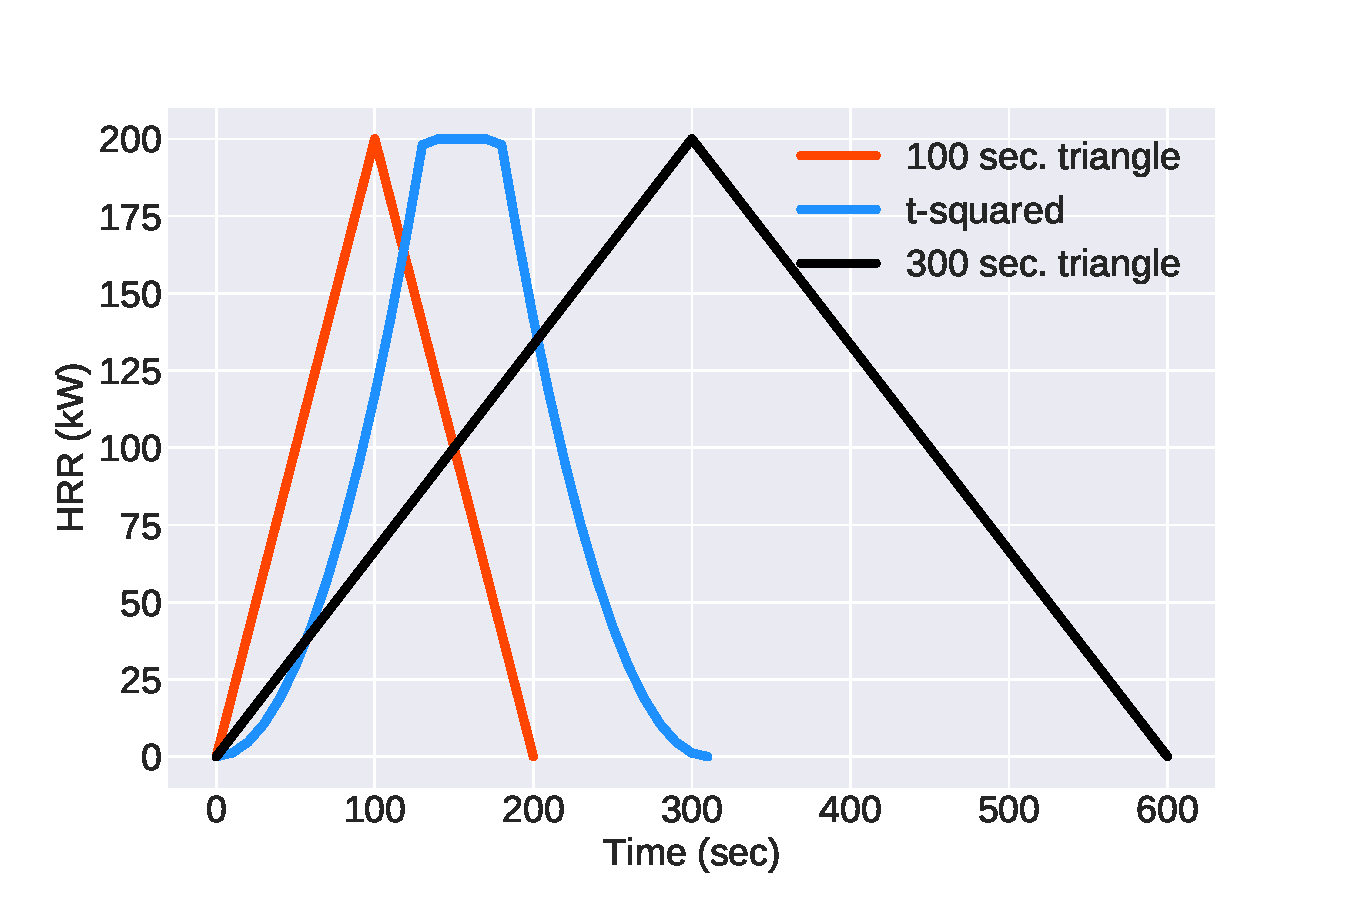
\includegraphics[width=\textwidth,keepaspectratio]{figures/training_ramps.pdf}
      \caption{Calibration HRR ramps}
      \label{fig:training_ramps}
  \end{subfigure}
  \begin{subfigure}[t]{.45\textwidth}
      \centering
      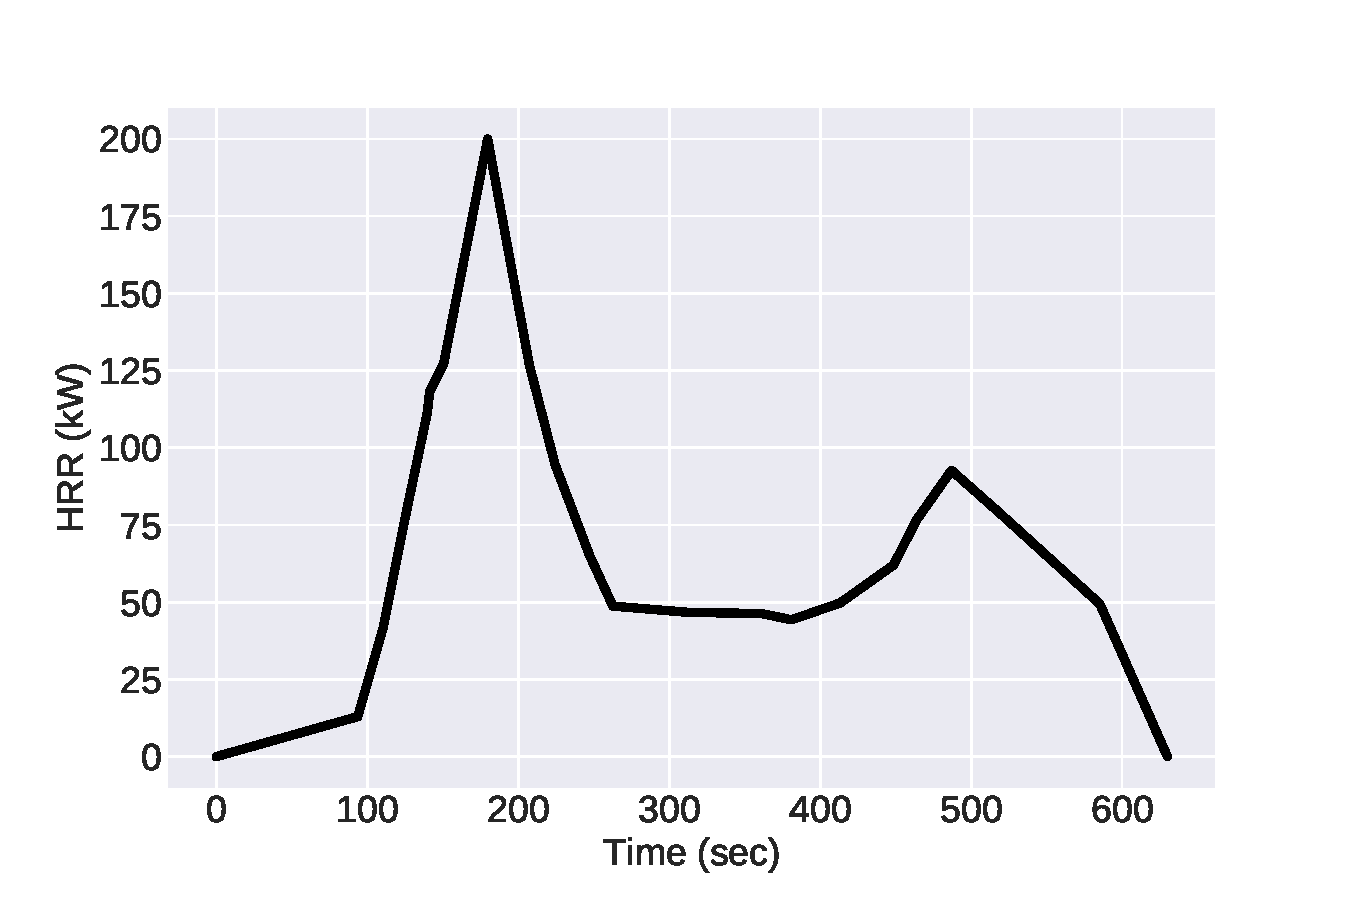
\includegraphics[width=\textwidth ,keepaspectratio]{figures/test_ramp.pdf}
      \caption{Test HRR ramp}
      \label{fig:test_ramp}
  \end{subfigure}
  \caption{\protect\ref{fig:training_ramps} shows the three HRR ramps used in the experiments that comprise the calibration set for the machine learning models. \protect\ref{fig:test_ramp} shows the HRR ramp used in the experiment that is used to evaluate the models. These ramps determine the setpoint for the flow rate of propane to the burner. However, the burner did not necessarily ignite immediately, so when the ramps are shown in later results, the HRR is assumed to be zero until ignition of the burner visually occurred. }
  \label{fig:hrr_ramps}
\end{figure}

The models are scored according the the mean absolute error (MAE), shown in equation \ref{eqn:mae},

\begin{equation}
  \label{eqn:mae}
  MAE = \frac{1}{N} \sum_{i=1}^N{|\dot{Q}_i - \dot{Q}^{\text{est}}_i|}
\end{equation}

\noindent where $\dot{Q}_i$ is the actual HRR, $\dot{Q}^{\text{est}}_i$ is the model's estimate of the HRR, and $N$ is the number of time points in the experiment. This can be expressed as a percentage by dividing the MAE by the mean HRR of the experiment. 

\subsection{Heat flux measurements}
This section describes machine learning methods for inferring the heat release rate of a compartment fire using heat flux measurements from the directional flame thermometers (DFTs) of the aforementioned experimental setup. Modak's point source model \cite{modak1977thermal} provides a simple and intuitive relationship between a fire's heat release rate and the resulting incident radiative heat flux on a nearby target. This model assumes that the radiative energy from a fire emanates isotropically from the center of a fire such that the incident radiative heat flux on a target is described by equation \ref{eqn:point_source},

 \begin{equation}
  \label{eqn:point_source}
  q'' = \frac{\chi_R\dot{Q}cos\theta}{4\pi R^2}
\end{equation}

where $q''$ is the incident radiative heat flux at a target located at a distance $R$ from the center of the fire, $\chi_R$ is the radiative fraction of the fire, and $\theta$ is the angle between the normal to the surface of the target and the line of sight between the target and the fire. Fleury \cite{fleury2010evaluation} also evaluated six different radiation models against experimental data and found the point source model to be the most accurate. Equation \ref{eqn:point_source} suggests that if the fire and sensors are kept at fixed locations, the radiative heat release rate, $\dot{Q}_R = \chi_R\dot{Q}$ is proportional to $q''$.  This linear proportionality motivates the use of linear statistical models.  For $d$ DFTs that each took $n$ measurements throughout an experiment at times $\boldsymbol{t^{\text{DFT}}} = \begin{bmatrix}  t^{\text{DFT}}_1 & t^{\text{DFT}}_2 & \ldots & t^{\text{DFT}}_n \end{bmatrix}^T$ the linear model is 


 \begin{equation}
  \label{eqn:linear_model_expanded}
 \begin{bmatrix}
  \dot{Q}_{R}(t^{\text{DFT}}_1) \\ 
  \dot{Q}_{R}(t^{\text{DFT}}_2) \\ 
  \vdots \\
  \dot{Q}_{R}(t^{\text{DFT}}_n) \\ 
  \end{bmatrix} = \begin{bmatrix}
  q''_1(t^{\text{DFT}}_1) & q''_2(t^{\text{DFT}}_1) & \cdots & q''_d(t^{\text{DFT}}_1) \\ 
  q''_1(t^{\text{DFT}}_2) & q''_2(t^{\text{DFT}}_2) & \cdots & q''_d(t^{\text{DFT}}_2) \\ 
  \vdots & \vdots & \vdots & \vdots \\ 
  q''_1(t^{\text{DFT}}_n) & q''_2(t^{\text{DFT}}_n) & \cdots & q''_d(t^{\text{DFT}}_n) \\ 
  \end{bmatrix}
   \begin{bmatrix}
  \beta_1 \\ 
  \beta_2 \\ 
  \vdots \\
  \beta_d \\ 
  \end{bmatrix} +
    \begin{bmatrix}
  \epsilon_1 \\ 
  \epsilon_2 \\ 
  \vdots \\
  \epsilon_n \\ 
  \end{bmatrix}
\end{equation}

\noindent or written more compactly as 

 \begin{equation}
  \label{eqn:linear_model}
    \boldsymbol{\dot{Q}}_{R}  = \boldsymbol{q}'' \boldsymbol{\beta} + \boldsymbol{\epsilon}
\end{equation}

For and experiment with $n$ observations and $d$ DFTs, $\boldsymbol{\dot{Q}}_{R} \in  \mathbb{R}^n$ is a vector of radiative HRR values, $\boldsymbol{q}'' \in \mathbb{R}^{n\text{x}m}$ is a matrix of heat flux measurements, $\boldsymbol{\beta} \in \mathbb{R}^n$ is a vector of regression slopes, and $\boldsymbol{\epsilon} \in \mathbb{R}^n$ is vector of random errors. Note that the model assumes that $\chi_R$ is constant throughout an experiment; it is not necessarily constant across different experiments if different fuels are used. If only one DFT were used, the point source model would suggest that $\beta = \frac{4 \pi R^2}{ cos \theta}$. However, this is not true for the multivariate case, and as a result, the coefficients of $\boldsymbol{\beta}$ are instead learned from the experimental data in the calibration set.

In addition to the theoretical explanation from Modak's point source model, the scatterplots shown in Figure \ref{fig:dft_scatterplot} show the linear relationship between the radiative heat release rate, $\boldsymbol{\dot{Q}}_{R}$ and $\boldsymbol{q}''$ from the calibration set experiments. 

\begin{figure}[htbp]
  \centering
  \begin{subfigure}[t]{.45\textwidth}
      \centering
      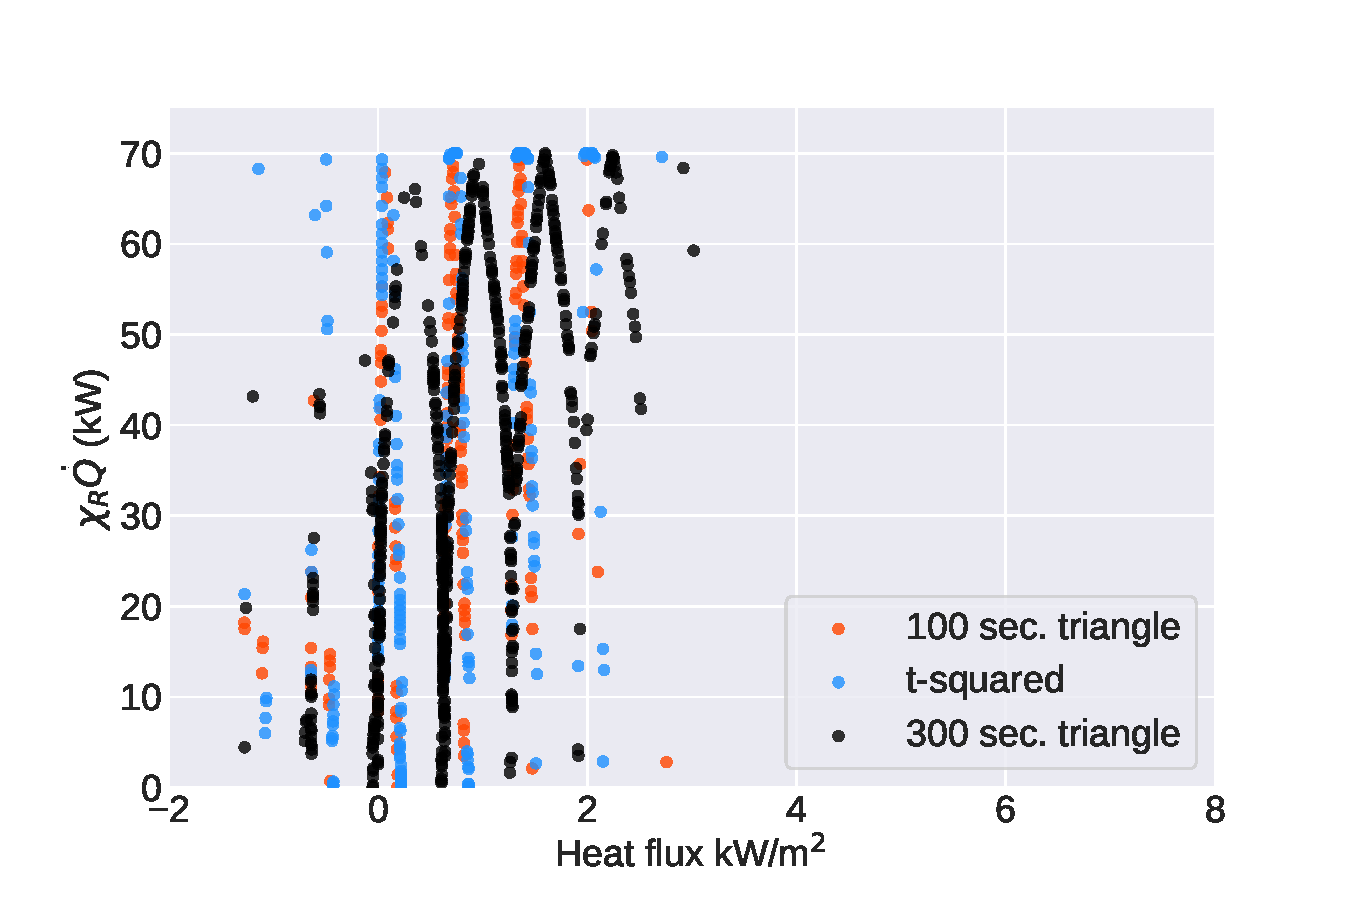
\includegraphics[width=\textwidth,keepaspectratio]{figures/weak_dft_scatter.pdf}
      \caption{Weak correlation}
      \label{fig:weak_scatter}
  \end{subfigure}
  \begin{subfigure}[t]{.45\textwidth}
      \centering
      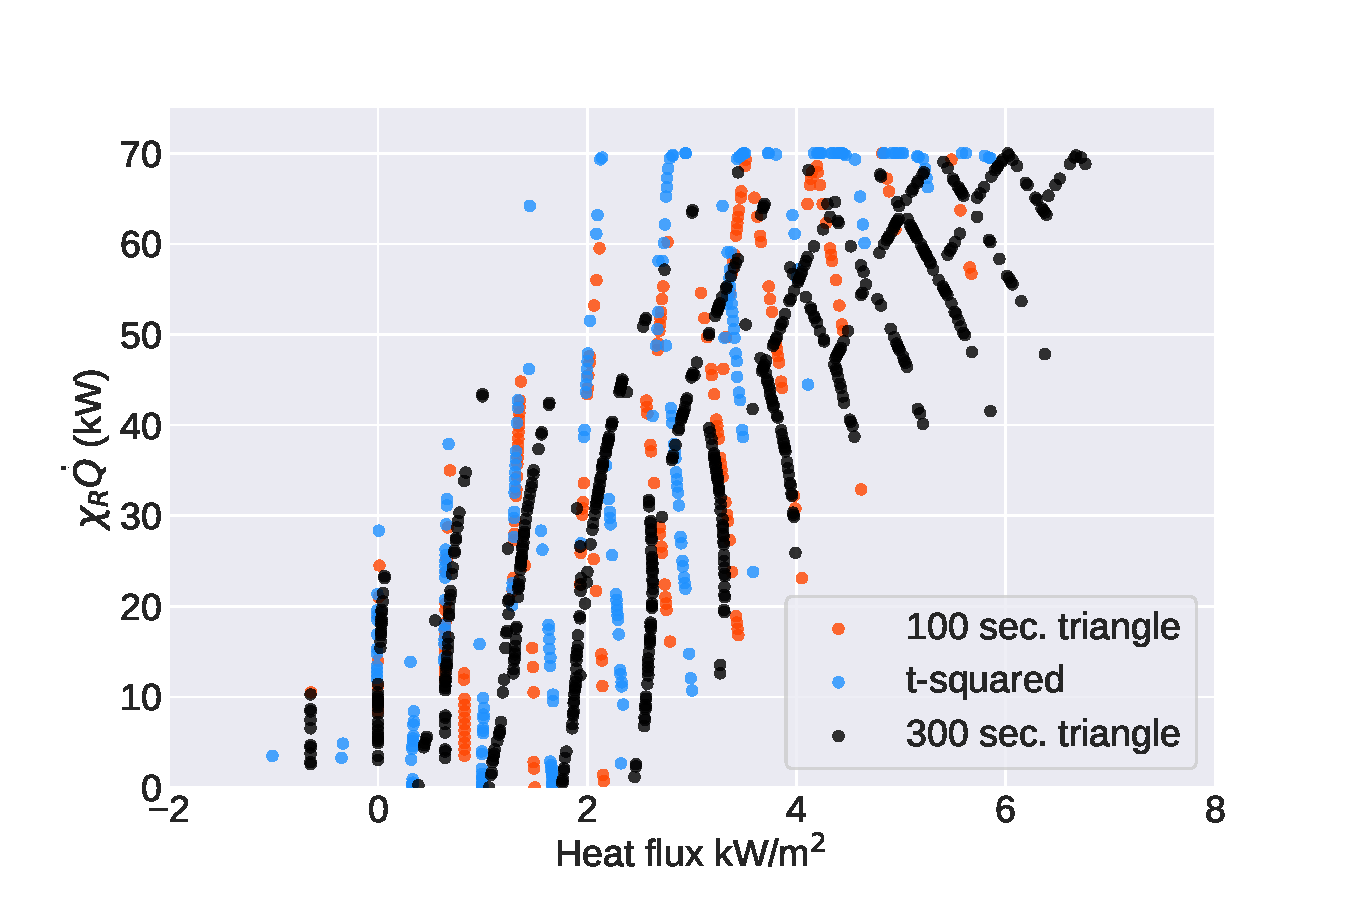
\includegraphics[width=\textwidth ,keepaspectratio]{figures/moderate_dft_scatter.pdf}
      \caption{Moderate correlation}
      \label{fig:moderate_scatter}
  \end{subfigure}
   \begin{subfigure}[t]{.45\textwidth}
      \centering
      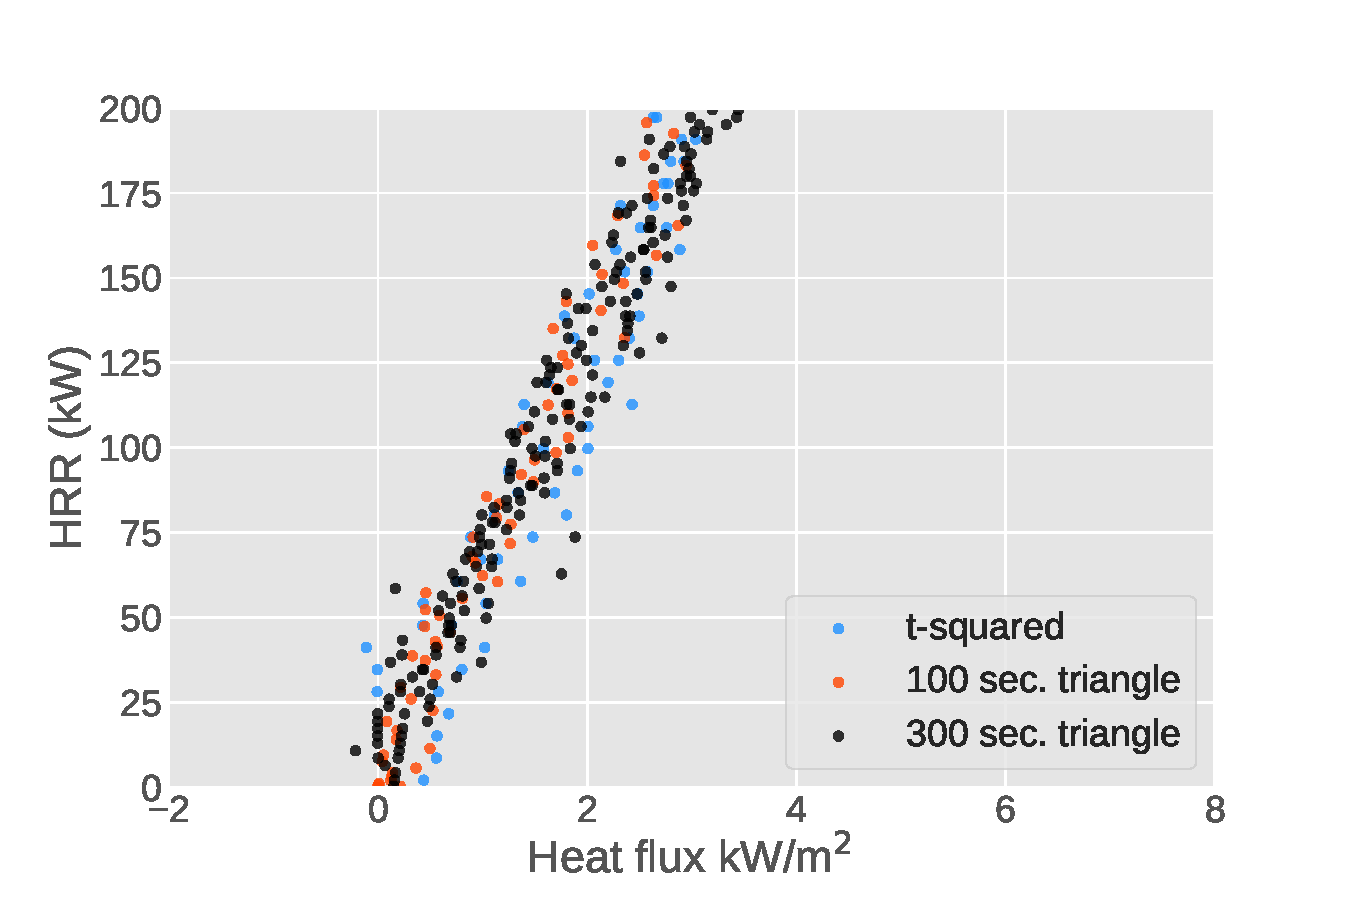
\includegraphics[width=\textwidth ,keepaspectratio]{figures/strong_dft_scatter.pdf}
      \caption{Strong correlation}
      \label{fig:strong_scatter}
  \end{subfigure}
  \caption{Scatterplots of the radiative heat release rate vs. measured heat flux for three different DFTs. These examples demonstrate the variation in the strength of correlations across DFTs. The measurement at each second of the calibration set experiments is shown.} 
  \label{fig:dft_scatterplot}
\end{figure}

The examples shown in Figure \ref{fig:dft_scatterplot} demonstrate how the strength of the correlation between the radiative HRR and measured heat flux varies significantly across the different DFTs. This finding raises several questions regarding the design of the model. First, should all the DFTs be included in the model? If not, which ones should be excluded and why? It may seem that the best set of sensors to include in the model is the one that includes only the DFTs whose measured heat flux is the most correlated with the radiative heat release rate. However, this is not necessarily true because multiple DFTs with strong correlations can provide redundant information. Also, the presence of multicollinearity can reduce the predictive accuracy of a linear regression model. This refers to the fact that the input features are correlated with each other; the measured heat fluxes will generally increase or decrease in parallel. 

To circumvent these issues, a lasso regression is employed using the Scikit-learn \cite{pedregosa2011scikit} package in Python . This technique is a modified linear regression that performs feature selection in addition to estimating values of $\boldsymbol{\beta}$. These values are estimated according to equation \ref{eqn:lasso}:

 \begin{equation}
  \label{eqn:lasso}
  \boldsymbol{\hat\beta}_{lasso} = \argmin_{\boldsymbol{\beta}}\Bigg\{ \underbrace{\big[\boldsymbol{\dot{Q}}_{R} - \boldsymbol{q}'' \boldsymbol{\beta}\big]^T\big[ \boldsymbol{\dot{Q}}_{R} - \boldsymbol{q}'' \boldsymbol{\beta}\big]}_{\text{I}} + \underbrace{\lambda||\boldsymbol{\beta}||_1}_{II}   \Bigg\}
\end{equation}

\noindent where $||\boldsymbol{\beta}||_1 = \sum_i{|\beta_i|}$ is the L1 norm of $\boldsymbol{\beta}$ and $\lambda$ is a hyperparameter that is learned from the data through 5-fold cross validation. This refers to the process of randomly splitting the training set into five different groups. For a given $\lambda$, lasso regression is fit using four of the five groups, and the model is scored based on its ability to make predictions on the excluded group. Specifically, the score is the coefficient of determination ($R^2$). This process is conducted five times so that each group is excluded once. The score for a given $\lambda$ is evaluated by averaging the scores across the five iterations of the cross validation and the $\lambda$ providing the best score is selected for the model. 

Note that term I is simply the sum of the squared residuals, meaning that if term II is zero, the process is identical to a ordinary least squares linear regression. The inclusion of term II, also known as L1 regularization, serves two purposes. First, it helps prevent overfitting as term II can be viewed as a penalty for increased model complexity. Second, it performs feature selection because the L1 regularization has a tendency to set values in $\boldsymbol{\beta}$ to zero, thereby removing the corresponding features from the model. It should be noted that the use of the $l^2$ norm (known as ridge regression, which is used later in this paper) is another common technique to combat overfitting; however, unlike lasso regression, ridge regression does not also perform feature selection. 

Figure \ref{fig:lasso_graphic} is a graphical illustration of the lasso regression framework. For a simple two variable regression model, $\boldsymbol{\dot{Q}}_{R} = q''_1\beta_1 + q''_2\beta_2$, the sum of the squared residuals, $[\boldsymbol{\dot{Q}}_{R} - \boldsymbol{q}'' \boldsymbol{\beta}\big]^T\big[\chi_R \boldsymbol{\dot{Q}}_{R} - \boldsymbol{q}'' \boldsymbol{\beta}]$, is the colored contour plot, whose minimum is indicated by the ``x" marker. If one were to perform an ordinary linear regression, the $\beta_1$ and $\beta_2$ that provide this optimum would be chosen. The lasso regression framework penalizes sets of $\boldsymbol{\beta}$ that are further away from the origin by a L1 or ''Manhattan" distance measure. A diamond comprises the set of locations that are a constant L1 distance from the origin, just as a circle would comprise the set of points that are a constant L2 distance from the origin. Intuitively, one can imagine a optimization problem in which the goal is to minimize the sum of the squared residuals while remaining within a specified L1 distance from the origin. The diamond shape of constant L1 contours gives the optimal $\beta$ a tendency to contain zeros. The black diamond marker indicates this optimum, which sets $\beta_2$ to zero, thereby removing $q''_2$ from the model. 

\begin{figure}[htb] \centering
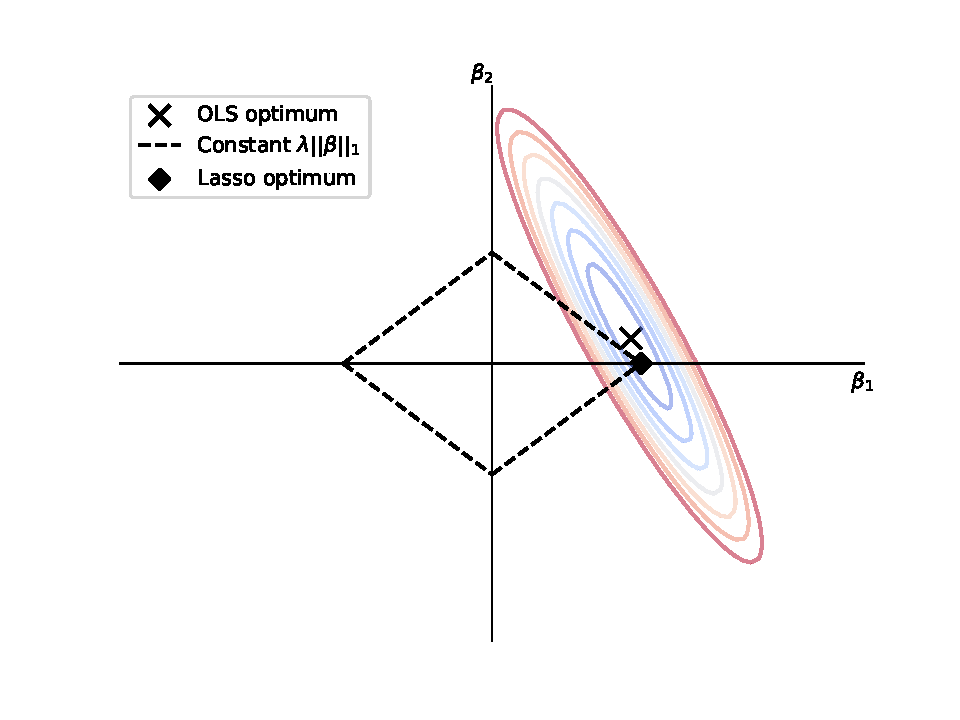
\includegraphics[width=.75\textwidth]{./figures/lasso_graphic.pdf}
\caption{A graphical illustration of the lasso regression framework. The colored contour plot shows the sum of the squared residual function, $[ \boldsymbol{\dot{Q}}_{R} - \boldsymbol{q}'' \boldsymbol{\beta}\big]^T\big[ \boldsymbol{\dot{Q}}_{R} - \boldsymbol{q}'' \boldsymbol{\beta}]$. The ``x" marker indicates the minimum of this function, which would determine $\boldsymbol{\beta}$ in an ordinary linear regression framework. However, in a lasso regression framework, there is a penalty for sets of coefficients that are further away from the origin according to the L1 distance. The dashed diamond comprises a set of points that are a constant L1 distance from the origin, and the black diamond marker indicates the solution to equation \protect\ref{eqn:lasso}.}
\label{fig:lasso_graphic}
\end{figure}

Figure \ref{fig:dft_regressions} shows a comparison of the predicted HRR curves produced by an ordinary linear regression (\ref{fig:linreg_rad}) and a lasso regression (\ref{fig:lasso_rad}).

\begin{figure}[htbp]
  \centering
  \begin{subfigure}[t]{.45\textwidth}
      \centering
      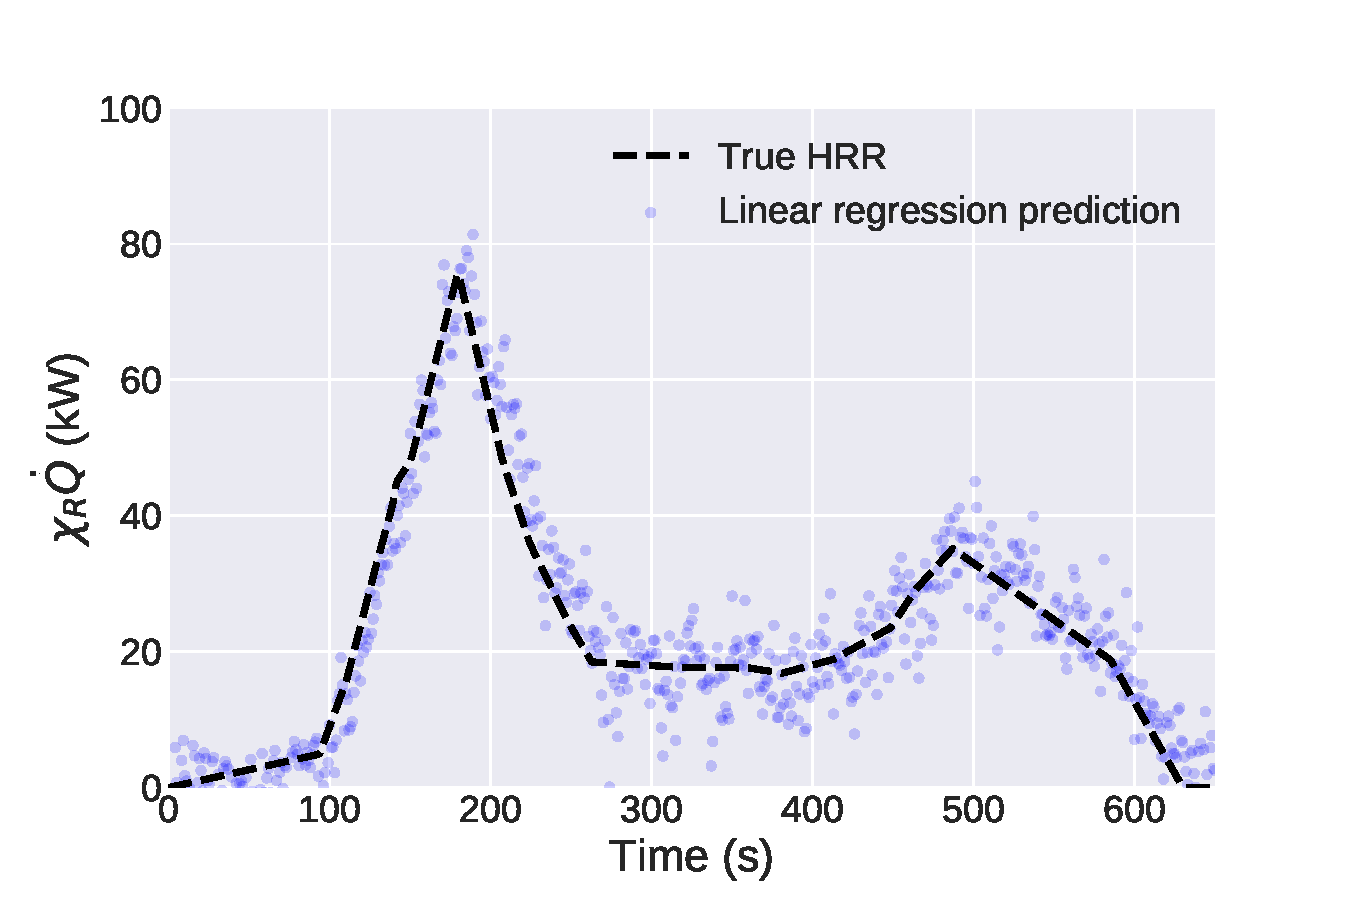
\includegraphics[width=\textwidth,keepaspectratio]{figures/linreg_rad.pdf}
      \caption{Linear regression (33 sensors) \\ MAE = 3.5 kW (16.6 \%)}
      \label{fig:linreg_rad}
  \end{subfigure}
  \begin{subfigure}[t]{.45\textwidth}
      \centering
      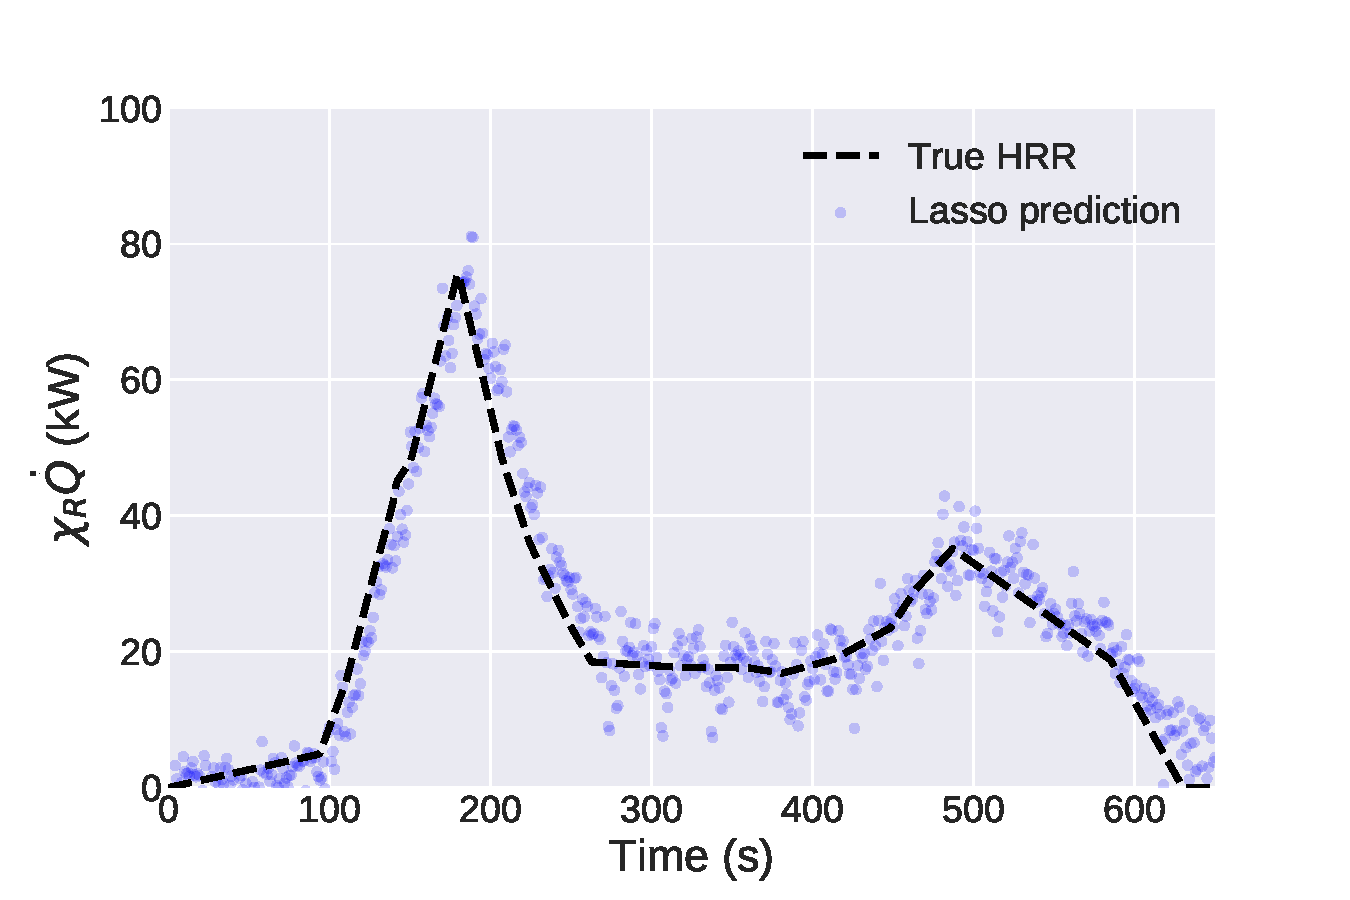
\includegraphics[width=\textwidth ,keepaspectratio]{figures/lasso_rad.pdf}
      \caption{Lasso regression (13 sensors) \\ MAE = 3.4 kW (15.9 \%)}
      \label{fig:lasso_rad}
  \end{subfigure}
  \caption{A comparison of the predicted HRR curves between an ordinary linear regression and a lasso regression. The mean absolute error add_value between the two approaches is similar, but the lasso regression is preferred because it uses only 13 DFTs as opposed to the linear regression which uses all 33 DFTs. } 
  \label{fig:dft_regressions}
\end{figure}

The lasso regression excludes 20 of the 33 DFTs from the model. Figure \ref{fig:lasso_dfts} shows locations of the DFTs included in the model and their corresponding regression coefficients ($\beta_i$).

\begin{figure}[htb] \centering
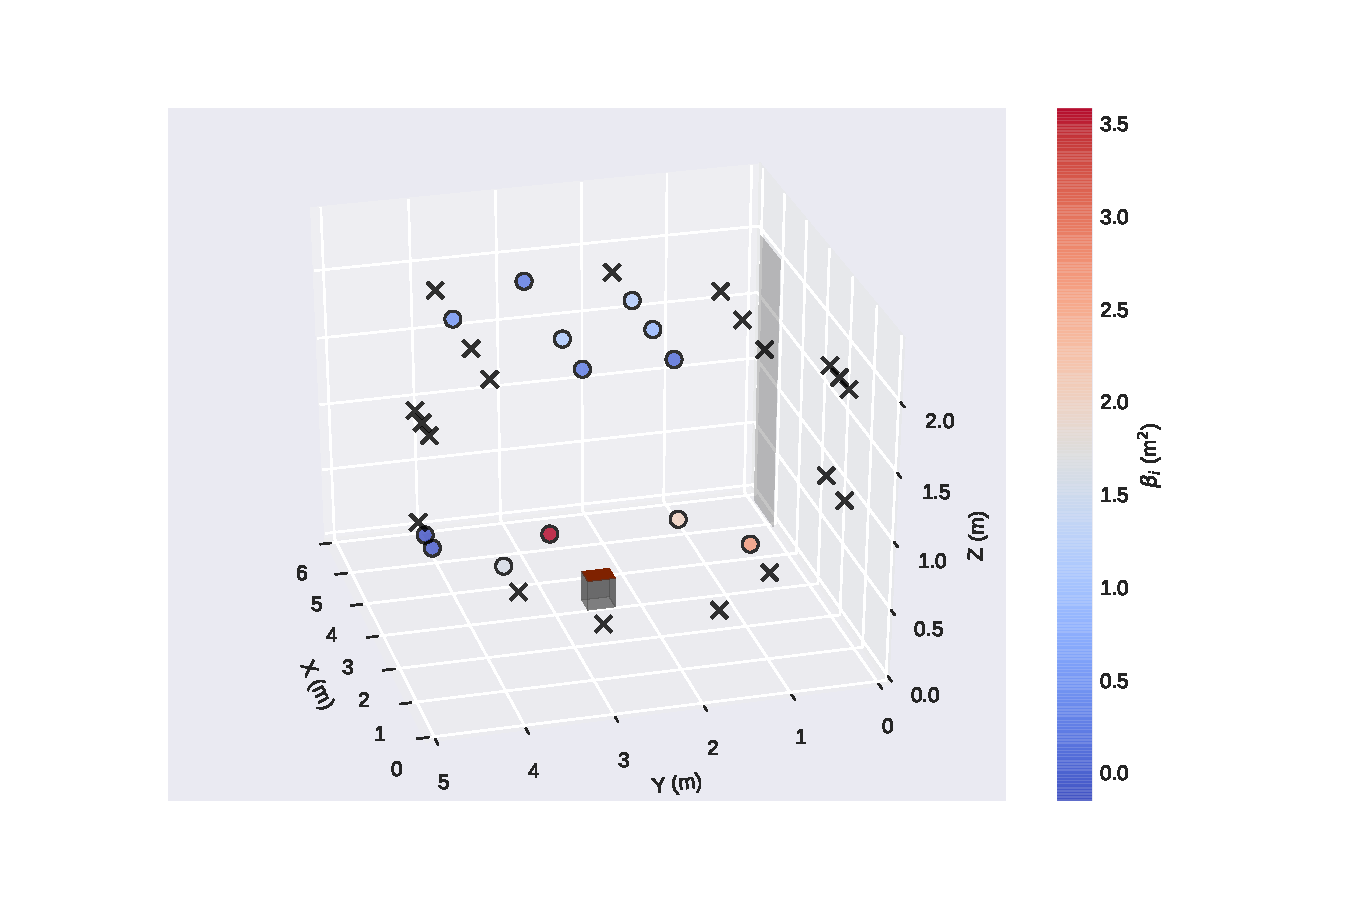
\includegraphics[width=.75\textwidth]{./figures/lasso_dfts.pdf}
\caption{A schematic of the of the burn structure and the DFTs with all DFT locations shown. The ``x" markers indicate DFTs that are excluded by the lasso regression. The circles indicate DFTs included in the lasso regression, and their color indicates the corresponding regression coefficient. The locations of the open door and the burner are also shown. Note the dimensions of $\beta_i$ are heat release rate per heat flux and the units are $m^2$.}
\label{fig:lasso_dfts}
\end{figure}

The lasso regression most greatly weights the heat fluxes of the low DFTs surrounding the burner in its predictions. This is not surprising given that these sensors are the closest to the burner, which likely means that their measurements are the most sensitive to the heat release rate. Also, because these sensors are low to the ground, they likely do not experience significant convective heating, which could introduce error. During the experiments, the authors noticed that the flame has a tendency to lean at different angles in the y-z plane, which could explain the relatively large weight placed into the DFT that lies in the negative-y direction from the burner. The inclusion of the DFTs near the ceiling is possibly due to the fact that the virtual radiation source of the fire grows with increasing HRR.

It should be noted that until this point, the model does not include any transient information, meaning that the lasso regression predicts $\boldsymbol{\dot{Q}}_{R}$ at an instant in time based on the measured heat fluxes at that same instant. It does not consider the history of heat fluxes nor the history of $\boldsymbol{\dot{Q}}_{R}$. As a result, the predictions significantly fluctuate over short timescales, but it is believed that the underlying HRR curve does not. This motivates the use of a temporal smoother to improve the predicted radiative HRR curve. Although there are many types of smoothers that could be used, the authors opted to use Gaussian process regression (also known as kriging) because it is a integral concept of later results in this paper. 

It is reasonable to expect that the lasso predictions are actually noisy draws centered around an underlying ``smoother" function. Mathematically, this can be written as

 \begin{equation}
  \label{eqn:gaussian_process_model}
  \dot{Q}_{R}^{\text{lasso}}(t) = \dot{Q}_{R}^{\text{GP}}(t) + \epsilon(t)
\end{equation}

where $\dot{Q}_{R}^{\text{lasso}}(t)$ is the lasso prediction at time $t$. The error, $\epsilon(t) \sim N(0,\sigma^2)$, is normally distributed with variance $\sigma^2$, and finally $\dot{Q}_{R}^{\text{GP}}(t)$ is the underlying function that Gaussian proccess regression (GPR) attempts to learn. A Gaussian process is a stochastic process in which any finite collection of random variables has a joint multivariate normal distribution \cite{lee2017deep}. Loosely speaking, a Gaussian process can be viewed as a probability distribution of functions, which may seem abstract to readers unfamiliar with this type of statistical modeling, especially because these functions do not have a specified form (linear, polynomial, etc). If one imagines a distribution of functions, then a random sample of $N$ functions could be collected from the distribution. Each of these functions could then be evaluated at some arbitrary time, $t_1$, producing a set of $N$ scalar values. If the distribution of functions meets the definition of a Gaussian process, then this sample of scalar values will reveal a univariate normal distribution (assuming $N$ is large enough to capture the population distribution). Similarly, these functions could be evaluated at two different times, $t_1, t_2$, and the vector of function evaluations would have a bivariate normal distribution. Any vector of $n$ function evaluations, $f(\boldsymbol{t})$, will follow a multivariate normal distribution, whose form is shown in equation \ref{eqn:multivariate_gaussian}.

 \begin{equation}
  \label{eqn:multivariate_gaussian}
  p\bigg(f(\boldsymbol{t}) \bigg) = \mathcal{N}\Big(\boldsymbol{\mu}, \boldsymbol{\Sigma} \Big) = 
  (2\pi)^{-\frac{n}{2}}\text{det}\big[\boldsymbol{\Sigma}\big]^{-\frac{1}{2}}\text{exp}\bigg(-\frac{1}{2}\big[f(\boldsymbol{t}) - \boldsymbol{\mu}\big]^T \boldsymbol{\Sigma}^{-1}\big[f(\boldsymbol{t}) - \boldsymbol{\mu}\big] \bigg)
\end{equation}

Just as a univariate normal distribution is uniquely characterized by a scalar mean and a scalar variance, a multivariate normal distribution is uniquely characterized by a mean vector $\boldsymbol{\mu}$ and a symmetirc positive semi-definite covariance matrix, $\boldsymbol{\Sigma}$, whose entries are described by equation \ref{eqn:covariance_matrix}.

 \begin{equation}
  \label{eqn:covariance_matrix}
  \Sigma_{i,j} = E\bigg([x_i- \mu_i][x_j - \mu_j] \bigg)
\end{equation}

\noindent where $E$ is the expectation operator, $E(x) =  \int_{-\infty}^{\infty} xp(x) dx$.




Going back to the thought experiment of drawing functions from a distribution, one can imagine drawing a random sample of $N$ functions and evaluating each function at the same two points, $t_i$ and $t_i + \Delta t$. If $\Delta t$ is small, then one would expect that the function evaluations at $t_i$ and $t_i + \Delta t$ would be similar (correlated), depending on how smooth the drawn functions are. In the limiting case, when $\Delta t = 0$, the function evaluations will be exactly the same (perfectly correlated) if the functions are continuous. Conversely, if $\Delta t$ is large, then the two quantities will generally be uncorrelated. This motivates the use of a function to quantify the covariance between function evaluations at different points based on the size of the interval between the two points. Specifically, the authors use a squared exponential kernel function, shown in equation \ref{eqn:squared_exponential}, 


 \begin{equation}
  \label{eqn:squared_exponential}
    K(t_i, t_j) = \tau^2exp\bigg(-\frac{(t_i-t_j)^2}{2b^2}\bigg)
\end{equation}

\noindent where $\tau^2$ is a hyperparameter that describes the magnitude of the function draws, and $b$, known as the bandwidth, relates to the time scale over which function evaluations are correlated. Intuitively, $b$ defines how smooth the function draws will be, with a larger bandwidth giving smoother functions. As previously noted, a mean vector and a covariance function uniquely characterize a multivariate normal distribution. Similarly, a mean function, $m$, and a kernel function, $K$, uniquely characterize a Gaussian process. For any vector of times $\boldsymbol{t} = \begin{bmatrix}  t_1 & t_2, & \ldots & t_n \end{bmatrix}^T$, if $f(t) \sim \mathcal{GP}(m,K)$, then $f(\boldsymbol{t}) \sim \mathcal{N}\Big(m(\boldsymbol{t}), \boldsymbol{\Sigma}\Big)$, where $\boldsymbol{\Sigma} =  K(\boldsymbol{t},\boldsymbol{t})$, i.e. $\Sigma_{i,j} = K(t_i, t_j)$. 

The concept of Gaussian processes allows for a flexible Bayesian regression framework. The general idea is that the uncertainty of an underlying function is described as a Gaussian process. A prior distribution is first constructed, describing a relatively wide variety of functions. However, many of these functions are unlikely given the degree of mismatch with the observed data as well as the assumptions made in equation \ref{eqn:gaussian_process_model}. Using Bayes' law, a posterior distribution for  $\dot{Q}_{R}^{\text{GP}}(t)$ is obtained. Although this distribution is not the distribution for the true radiative HRR, $\dot{Q}_{R}(t)$, it produces significantly more accurate estimations of $\dot{Q}_{R}(t)$ than the lasso framework does in isolation. 

The first step in the methodology is to define a prior for $\dot{Q}_{R}^{\text{GP}}(t)$. A common choice for a prior is a Gaussian process with mean zero \cite{rasmussen2003gaussian}, i.e. $\dot{Q}_{R}^{\text{GP}}(t) \sim \mathcal{GP}(0, K)$ The astute reader may notice that the prior is not yet fully defined because the hyperparameters, $\tau^2$ and $b$, have not been specified in the kernel function (equation \ref{eqn:squared_exponential}). One approach would be to specify priors for these parameters, resulting in a fully Bayesian Gaussian process regression model. For simplicity, the authors instead opt to determine these parameters by maximizing the marginal likelihood, which is again a common practice \cite{rasmussen2003gaussian}. The idea behind this approach is to choose the $\tau^2$ and $b$ that generate the prior distribution that is most likely to produce the observed data given the assumptions of equation \ref{eqn:gaussian_process_model}. Recall that lasso predictions are computed for every time in the vector $\boldsymbol{t^{\text{DFT}}} = \begin{bmatrix}  t^{\text{DFT}}_1 & t^{\text{DFT}}_2 & \ldots & t^{\text{DFT}}_n \end{bmatrix}^T$. Given the Gaussian process prior, the distribution of function evaluations for these times is multivariate normal. Specifically,  $\dot{Q}_{R}^{\text{GP}}(\boldsymbol{t^{\text{DFT}}}) \sim \mathcal{N}\Big(\boldsymbol{0}, \  K( \boldsymbol{t^{\text{DFT}}}, \boldsymbol{t^{\text{DFT}}}, \tau^2, b) \Big)$ Note the explicit indication of the fact that the covariance matrix returned by the kernel function depends on the hyperparameters $\tau^2$ and $b$. Recall that the lasso predictions, $\dot{Q}_{R}^{\text{lasso}}(\boldsymbol{t^{\text{DFT}}})$,  are assumed to be $\dot{Q}_{R}^{\text{GP}}(\boldsymbol{t^{\text{DFT}}})$ plus a vector of random Gaussian noise, $\boldsymbol{\epsilon} \sim \mathcal{N}(\boldsymbol{0}, \sigma^2\boldsymbol{I})$, where $\boldsymbol{I}$ is the identity matrix. The variance $\sigma^2$ can be estimated by examining the scatter of the lasso predictions around the true HRR for an experiment in the calibration set according to equation \ref{eqn:sigma_estimate}: 

 \begin{equation}
  \label{eqn:sigma_estimate}
    \sigma^2 \approx \sum_{i=1}^{N_{exp}}\frac{\Big[\dot{Q}_{R}^{\text{lasso}}(t^{\text{DFT}}_i) - \dot{Q}_{R}(t_i^{\text{DFT}})\Big]^2}{N_{exp}-1} 
\end{equation}

\noindent where $N_{exp}$ is the length of $\boldsymbol{t}^{\text{DFT}}$ for the experiment used for this estimation. The authors used the 100 second triangle fire for this calculation, but the results are similar regardless of which experiment is chosen. Technically $\sigma^2$ is the variance of the lasso predictions around $\dot{Q}_{R}^{\text{GP}}(t)$ rather than the true radiative HRR, $\dot{Q}_{R}(t_i^{\text{DFT}})$, but equation \ref{eqn:sigma_estimate} is a convenient approximation. Also, recall that $\dot{Q}_{R}(\boldsymbol{t}^{\text{DFT}})$ is known for the experiments in the calibration set because they are viewed as calibration experiments.


 Because $\dot{Q}_{R}^{\text{lasso}}(\boldsymbol{t^{\text{DFT}}})$ is the sum of two (multivariate) normally distributed random variables, it is also normally distributed; its mean vector is the sum of the two mean vectors and its covariance matrix is the sum of the two covariance matrices, i.e. $\dot{Q}_{R}^{\text{lasso}}(\boldsymbol{t^{\text{DFT}}}) \sim \mathcal{N}\Big(\boldsymbol{0}, \ K( \boldsymbol{t^{\text{DFT}}}, \boldsymbol{t^{\text{DFT}}}, \tau^2, b) + \sigma^2\boldsymbol{I} \Big)$. Therefore the probability density function (PDF), $p\Big(\dot{Q}_{R}^{\text{lasso}}(\boldsymbol{t^{\text{DFT}}}), \tau, b \Big)$, follows the form of equation \ref{eqn:multivariate_gaussian}. Plugging in the vector of observed lasso predictions for and individual experiment gives a scalar probability density, or \textit{likelihood}, that depends on $\tau^2$ and $b$. Using a Nelder-Mead optimization algorithm \cite{nelder1965simplex} implemented in the python package Scipy \cite{jones2001scipy}, the optimal hyperparameters, $\tau^2_{\text{opt}}$ and $b_{\text{opt}}$ are chosen according to equation \ref{eqn:max_likelihood}. The initial guess for $b$ is 10 seconds and the initial guess for $\tau^2$ is 5,000 kW$^2$. 

\begin{equation}
  \label{eqn:max_likelihood}
  \tau^2_{\text{opt}}, \ b_{\text{opt}} = 
  \argmax_{\tau^2, b} \Bigg\{log\bigg[ p\Big(\dot{Q}_{R}^{\text{lasso}}(\boldsymbol{t^{\text{DFT}}}), \tau, b \Big)\bigg] \Bigg\}
\end{equation}

Once the hyperparameters are optimized, the prior is fully specified. Figure \ref{fig:gp_prior} shows five functions drawn from the Gaussian process (sampled every second). The next step is to update the prior given the observed data using Bayes' law. Specifically, the objective is to compute the probability distribution of $\dot{Q}_{R}^{\text{GP}}(\boldsymbol{t^{*}})$ evaluated at an arbitrary vector of times, $\boldsymbol{t}^* = \begin{bmatrix}  t^*_1 & t^*_2 & \ldots & t^*_p \end{bmatrix}^T$ given the prior and the observed lasso predictions evaluated at $\boldsymbol{t^{\text{DFT}}}$. Given that $\dot{Q}_{R}^{\text{GP}}(t) \sim \mathcal{GP}(0,K_{\text{opt}})$, where $K_{\text{opt}}$ indicates the kernel function with optimized hyperparameters, the function evaluations for any vector of times produces a multivariate normal distribution. If $\boldsymbol{t^{\text{DFT}}}$ and $\boldsymbol{t^{*}}$ are concatenated into a single vector, $\begin{bmatrix} \boldsymbol{t^{\text{DFT}}} & \boldsymbol{t^{*}} \end{bmatrix}^T \in \mathbb{R}^{n+p}$, then the corresponding joint distribution of function evaluations can be written as 

\begin{equation}
  \label{eqn:joint_GP}
  \begin{bmatrix}
  \dot{Q}_{R}^{\text{GP}}(\boldsymbol{t}^{\text{DFT}}) \\
  \dot{Q}_{R}^{\text{GP}}(\boldsymbol{t}^*)
  \end{bmatrix} \sim 
  \mathcal{N} \Bigg(\boldsymbol{0}, 
  \begin{bmatrix}
 K_{\text{opt}}(\boldsymbol{t}^{\text{DFT}}, \boldsymbol{t}^{\text{DFT}}) & K_{\text{opt}}(\boldsymbol{t}^{\text{DFT}}, \boldsymbol{t}^*) \\ 
   K_{\text{opt}}(\boldsymbol{t}^*, \boldsymbol{t}^{\text{DFT}}) &  K_{\text{opt}}(\boldsymbol{t}^*, \boldsymbol{t}^*) 
  \end{bmatrix}
  \Bigg)
\end{equation}

Note that the $n$+$p$ by $n$+$p$ covariance matrix is shown as a block matrix comprised of four smaller matrices. As previously stated, equation \ref{eqn:gaussian_process_model} indicates that   $\dot{Q}_{R}^{\text{lasso}}(\boldsymbol{t^{\text{DFT}}}) \sim \mathcal{N}\Big(\boldsymbol{0}, \ K_{\text{opt}}( \boldsymbol{t^{\text{DFT}}}, \boldsymbol{t^{\text{DFT}}}) + \sigma^2\boldsymbol{I} \Big)$, which allows equation \ref{eqn:joint_GP} to be expressed in terms of the lasso predictions, $\dot{Q}_{R}^{\text{lasso}}(\boldsymbol{t^{\text{DFT}}})$, shown below:


\begin{equation}
  \label{eqn:joint_GP_lasso}
  \begin{bmatrix}
  \dot{Q}_{R}^{\text{lasso}}(\boldsymbol{t}^{\text{DFT}}) \\
  \dot{Q}_{R}^{\text{GP}}(\boldsymbol{t}^*)
  \end{bmatrix} \sim 
  \mathcal{N} \Bigg(\boldsymbol{0}, 
  \begin{bmatrix}
 K_{\text{opt}}(\boldsymbol{t}^{\text{DFT}}, \boldsymbol{t}^{\text{DFT}}) + \sigma^2\boldsymbol{I}& K_{\text{opt}}(\boldsymbol{t}^{\text{DFT}}, \boldsymbol{t}^*) \\ 
   K_{\text{opt}}(\boldsymbol{t}^*, \boldsymbol{t}^{\text{DFT}}) &  K_{\text{opt}}(\boldsymbol{t}^*, \boldsymbol{t}^*) 
  \end{bmatrix}
  \Bigg)
\end{equation}

Equation \ref{eqn:joint_GP_lasso} describes the joint distribution of $\dot{Q}_{R}^{\text{lasso}}(\boldsymbol{t}^{\text{DFT}})$ and $\dot{Q}_{R}^{\text{GP}}(\boldsymbol{t}^*)$, meaning that one can concatenate these two vectors together, compute the covariance matrix, and then obtain an expression for $p\Big(\dot{Q}_{R}^{\text{lasso}}(\boldsymbol{t}^{\text{DFT}}), \  \dot{Q}_{R}^{\text{GP}}(\boldsymbol{t}^*)\Big)$, the probability density for the concatenated vector, using equation \ref{eqn:multivariate_gaussian}. Recall that the first $n$ entries in this concatenated vector are known because they are the lasso predictions, and the goal is to learn the distribution for the remaining $p$ entries, i.e. the conditional probability distribution, $p\Big(\dot{Q}_{R}^{\text{GP}}(\boldsymbol{t}^*)  \Big| \dot{Q}_{R}^{\text{lasso}}(\boldsymbol{t}^{\text{DFT}})  \Big)$. Using Bayes' law, 

$$
p\Big(\dot{Q}_{R}^{\text{GP}}(\boldsymbol{t}^*)  \Big| \dot{Q}_{R}^{\text{lasso}}(\boldsymbol{t}^{\text{DFT}})  \Big) = \frac{p\Big(\dot{Q}_{R}^{\text{lasso}}(\boldsymbol{t}^{\text{DFT}})  \Big| \dot{Q}_{R}^{\text{GP}}(\boldsymbol{t}^*)\Big) p\Big(\dot{Q}_{R}^{\text{GP}}(\boldsymbol{t}^*)\Big)}{p\Big(\dot{Q}_{R}^{\text{lasso}}(\boldsymbol{t}^{\text{DFT}})\Big)}
$$

\begin{equation}
  \label{eqn:bayes_joint}
 = \frac{p\Big(\dot{Q}_{R}^{\text{lasso}}(\boldsymbol{t}^{\text{DFT}}), \  \dot{Q}_{R}^{\text{GP}}(\boldsymbol{t}^*)\Big)}{p\Big(\dot{Q}_{R}^{\text{lasso}}(\boldsymbol{t}^{\text{DFT}})\Big)}
\end{equation}

The numerator of equation \ref{eqn:bayes_joint} is described by equation \ref{eqn:joint_GP_lasso}. The denominator is again $\dot{Q}_{R}^{\text{lasso}}(\boldsymbol{t^{\text{DFT}}}) \sim \mathcal{N}\Big(\boldsymbol{0}, \ K_{\text{opt}}( \boldsymbol{t^{\text{DFT}}}, \boldsymbol{t^{\text{DFT}}}) + \sigma^2\boldsymbol{I} \Big)$. Though the matrix algebra is not trivial, it can be shown that dividing these two multivariate normal PDFs results in another multivariate normal PDF,

\begin{equation}
  \label{eqn:gp_posterior}
 \dot{Q}_{R}^{\text{GP}}(\boldsymbol{t}^*)  \Big| \dot{Q}_{R}^{\text{lasso}}(\boldsymbol{t}^{\text{DFT}}) \sim 
 \mathcal{N}\Big(\boldsymbol{m}_{post}, \boldsymbol{C}_{post}\Big)
\end{equation}

\noindent where

$$
\boldsymbol{m}_{post} = K_{\text{opt}}(\boldsymbol{t}^*, \boldsymbol{t}^{\text{DFT}})\Big[K_{\text{opt}}(\boldsymbol{t}^{\text{DFT}}, \boldsymbol{t}^{\text{DFT}}) + \sigma^2\boldsymbol{I}\Big]^{-1} \dot{Q}_{R}^{\text{lasso}}(\boldsymbol{t}^{\text{DFT}})
$$

\noindent and 

$$
\boldsymbol{C}_{post} = K_{\text{opt}}(\boldsymbol{t}^*, \boldsymbol{t}^*) -  K_{\text{opt}}( \boldsymbol{t}^*, \boldsymbol{t}^{\text{DFT}})\Big[K_{\text{opt}}(\boldsymbol{t}^{\text{DFT}}, \boldsymbol{t}^{\text{DFT}}) + \sigma^2\boldsymbol{I}\Big]^{-1}K_{\text{opt}}(\boldsymbol{t}^{\text{DFT}},\boldsymbol{t}^*)
$$


Five draws from the posterior distribution calculated with equation \ref{eqn:gp_posterior} are shown in \ref{fig:gp_posterior}. The draws from the posterior generally reconstruct the true experimental radiative HRR curve better than the relatively noisy lasso predictions, demonstrating the utility of the ensemble regression methodology. From this point on, the mean of the posterior distribution, $\boldsymbol{m}_{post}$ is used as the estimate of $\dot{Q}_R(t)$. 

\begin{figure}[htbp]
  \centering
  \begin{subfigure}[t]{.45\textwidth}
      \centering
      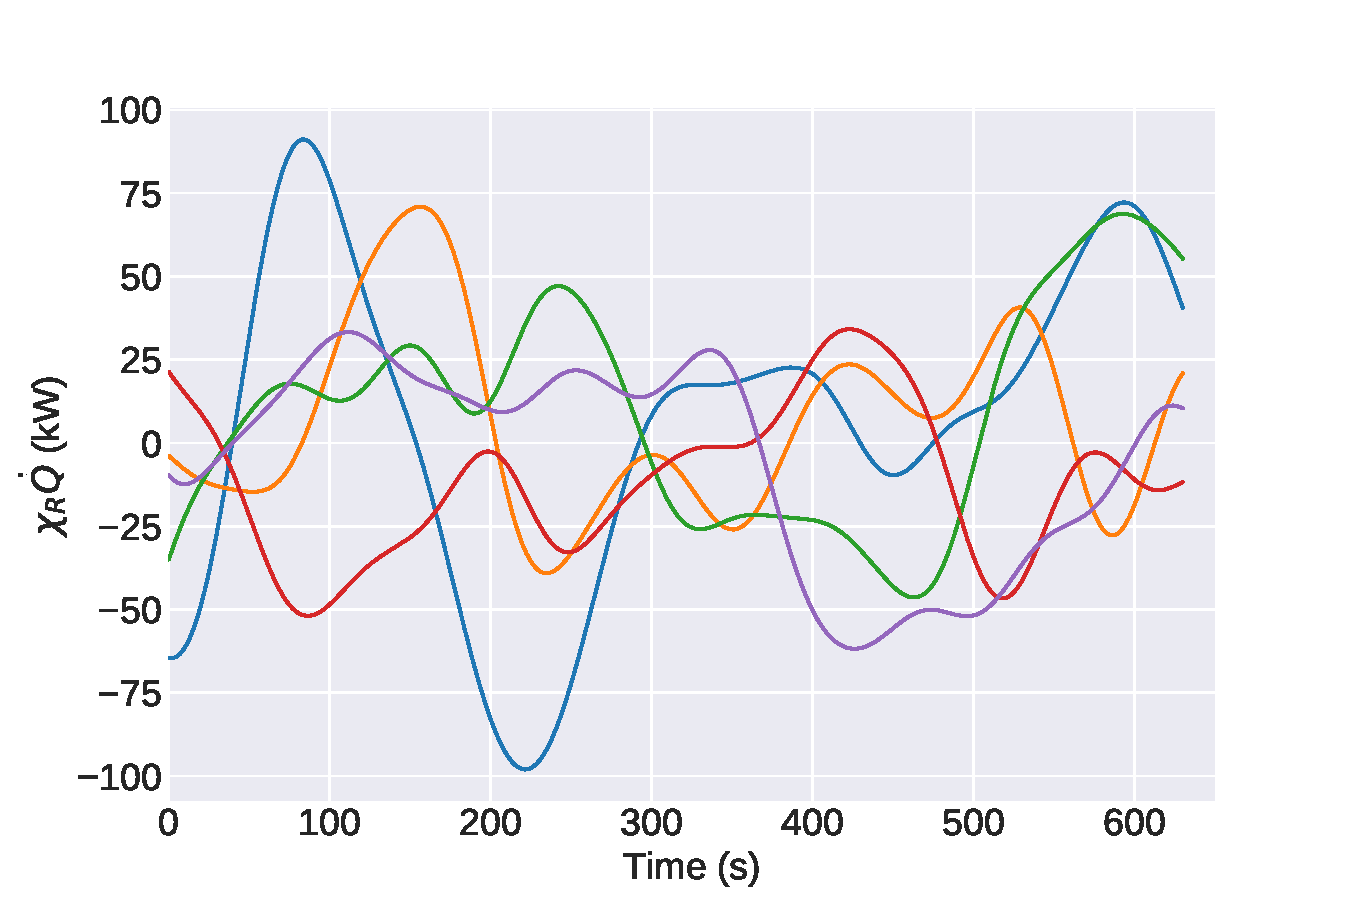
\includegraphics[width=\textwidth,keepaspectratio]{figures/gp_prior.pdf}
      \caption{Five draws from the prior with optimized hyperparameters.}
      \label{fig:gp_prior}
  \end{subfigure}
  \begin{subfigure}[t]{.45\textwidth}
      \centering
      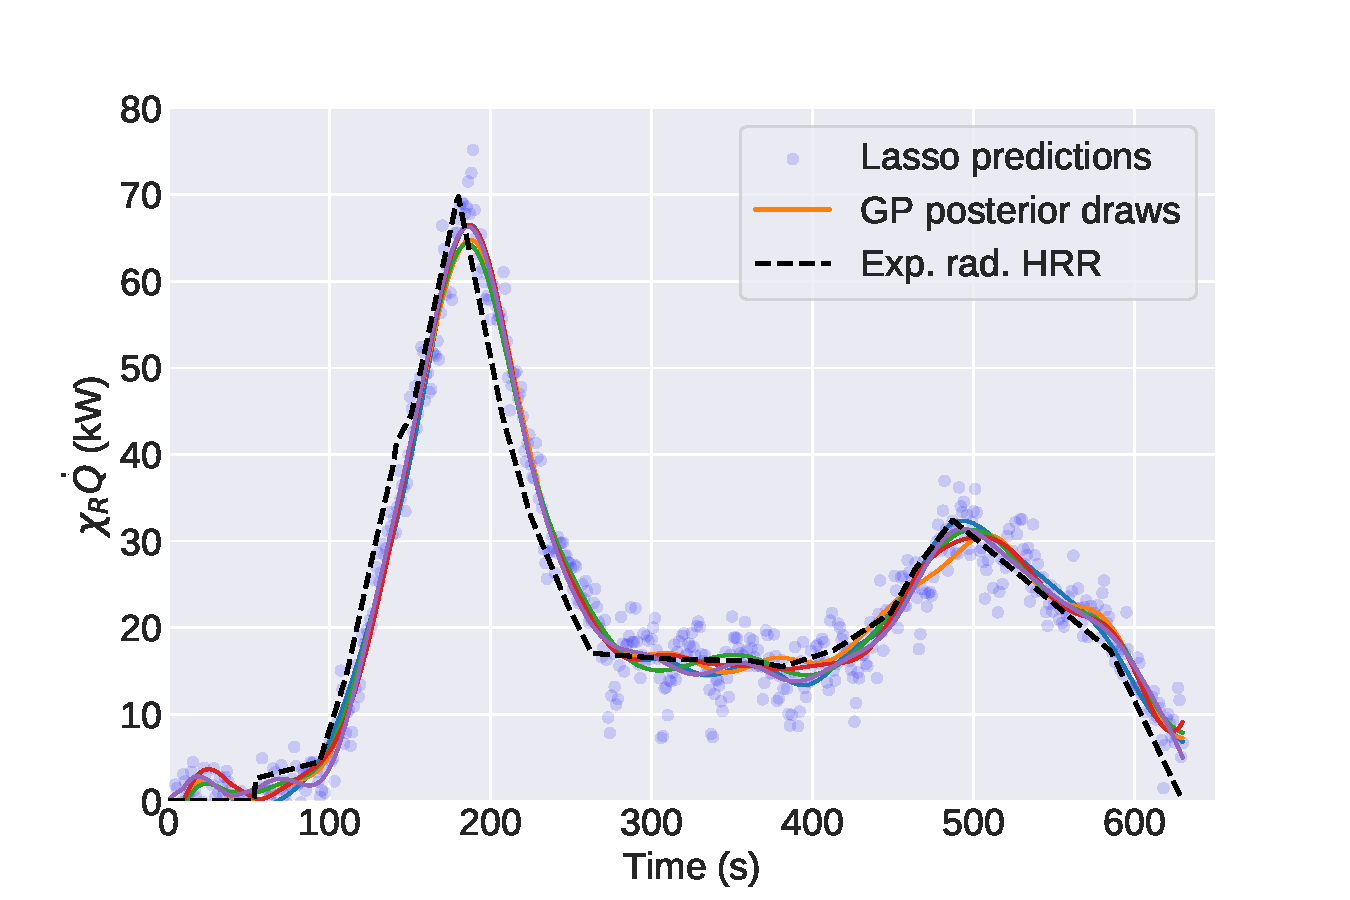
\includegraphics[width=\textwidth ,keepaspectratio]{figures/gp_posterior.pdf}
      \caption{Five draws from the posterior distribution.}
      \label{fig:gp_posterior}
  \end{subfigure}
  \caption{A visual depiction of the Gaussian process methodology. Figure \protect\ref{fig:gp_prior} shows five random draws from the Gaussian process prior with optimized hyperparameters. Using Bayes' law, the GPR methodology updates this distribution of functions given the lasso predictions. The resulting distribution of functions produces more accurate reconstructions of the true radiative HRR curve than the lasso model does by itself.} 
  \label{fig:gp_regression_example}
\end{figure}

In order to gain a better idea of the the ability of this framework to measure radiative HRR curves, the methodology described in this section is conducted four times with each of the four experiments serving as the test case once. The model trains on the other three experiments and predicts the HRR curve for the test experiment. These results are shown in Figure \ref{fig:dft_gp_results}.

\begin{figure}[htbp]
  \centering
  \begin{subfigure}[t]{.45\textwidth}
      \centering
      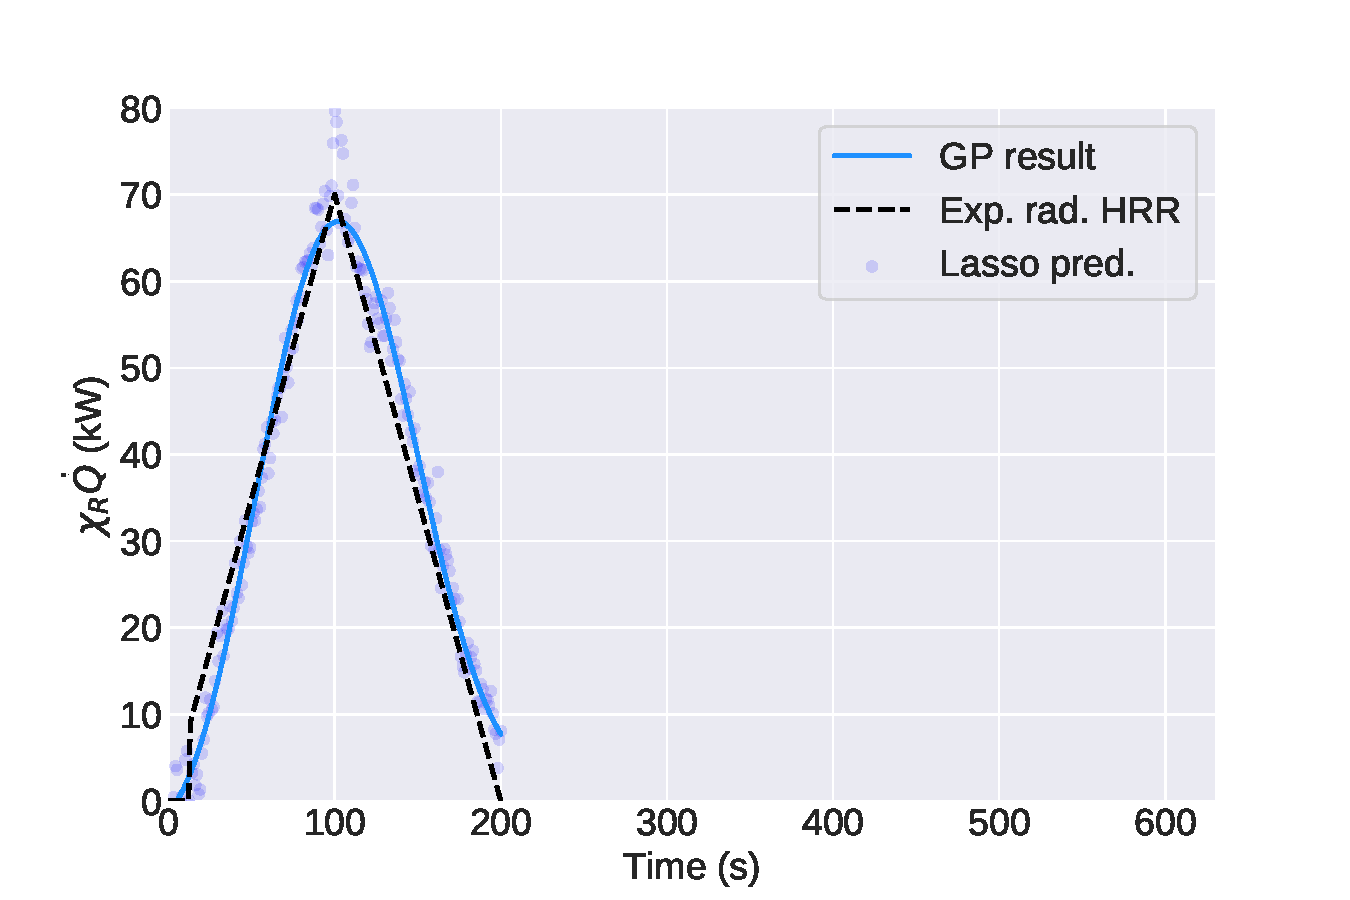
\includegraphics[width=\textwidth,keepaspectratio]{figures/dft_result_100s_triangle.pdf}
      \caption{100 sec. triangle \\ MAE = 3.9 kW (11.2 \%) }
      \label{fig:dft_result_100s_triangle}
  \end{subfigure}
  \begin{subfigure}[t]{.45\textwidth}
      \centering
      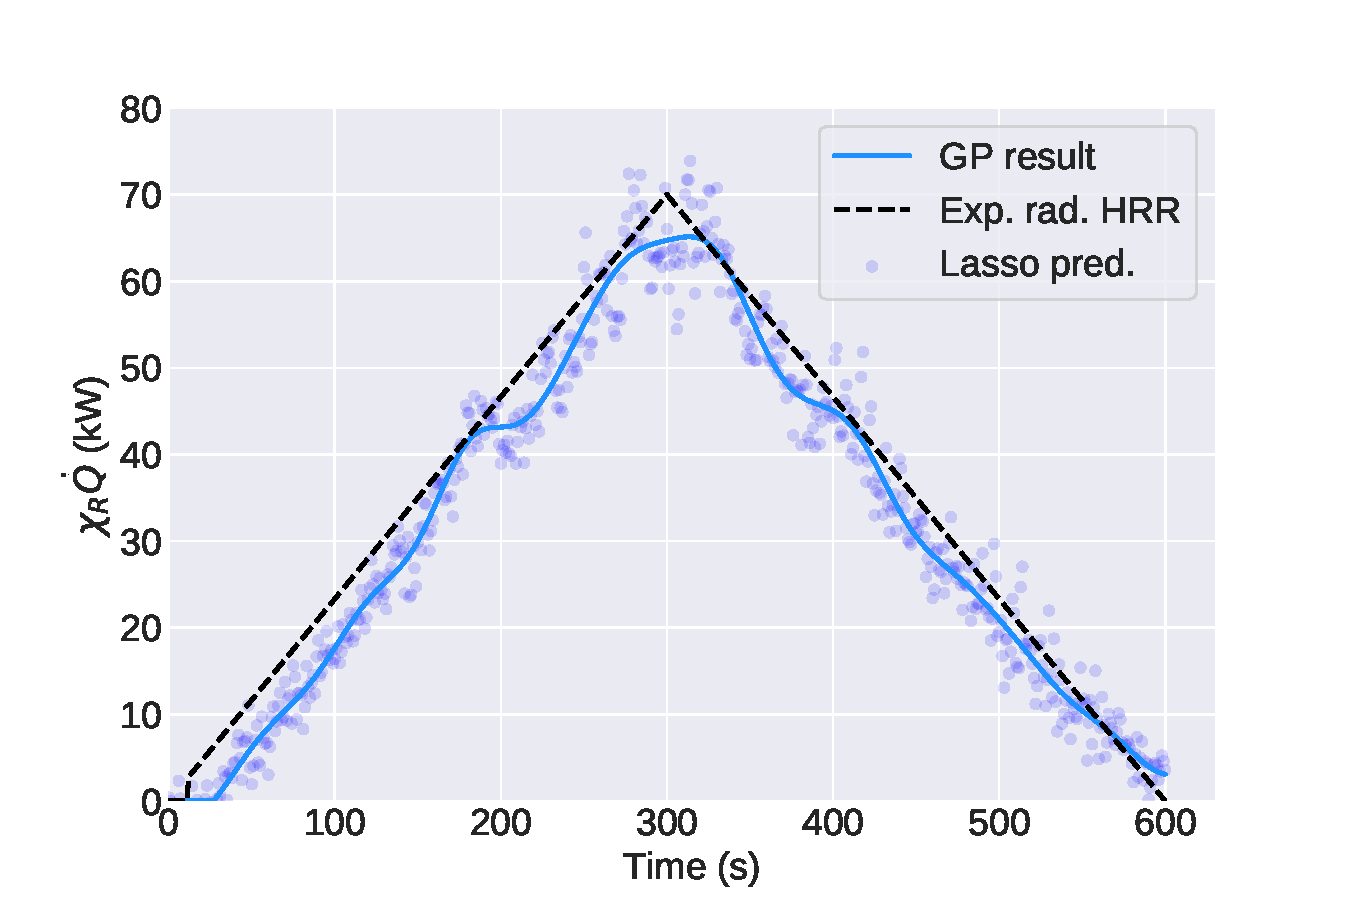
\includegraphics[width=\textwidth ,keepaspectratio]{figures/dft_result_300s_triangle.pdf}
      \caption{300 sec. triangle \\ MAE = 3.3 kW (9.3 \%)}
      \label{fig:dft_result_300s_triangle}
  \end{subfigure}
   \begin{subfigure}[t]{.45\textwidth}
      \centering
      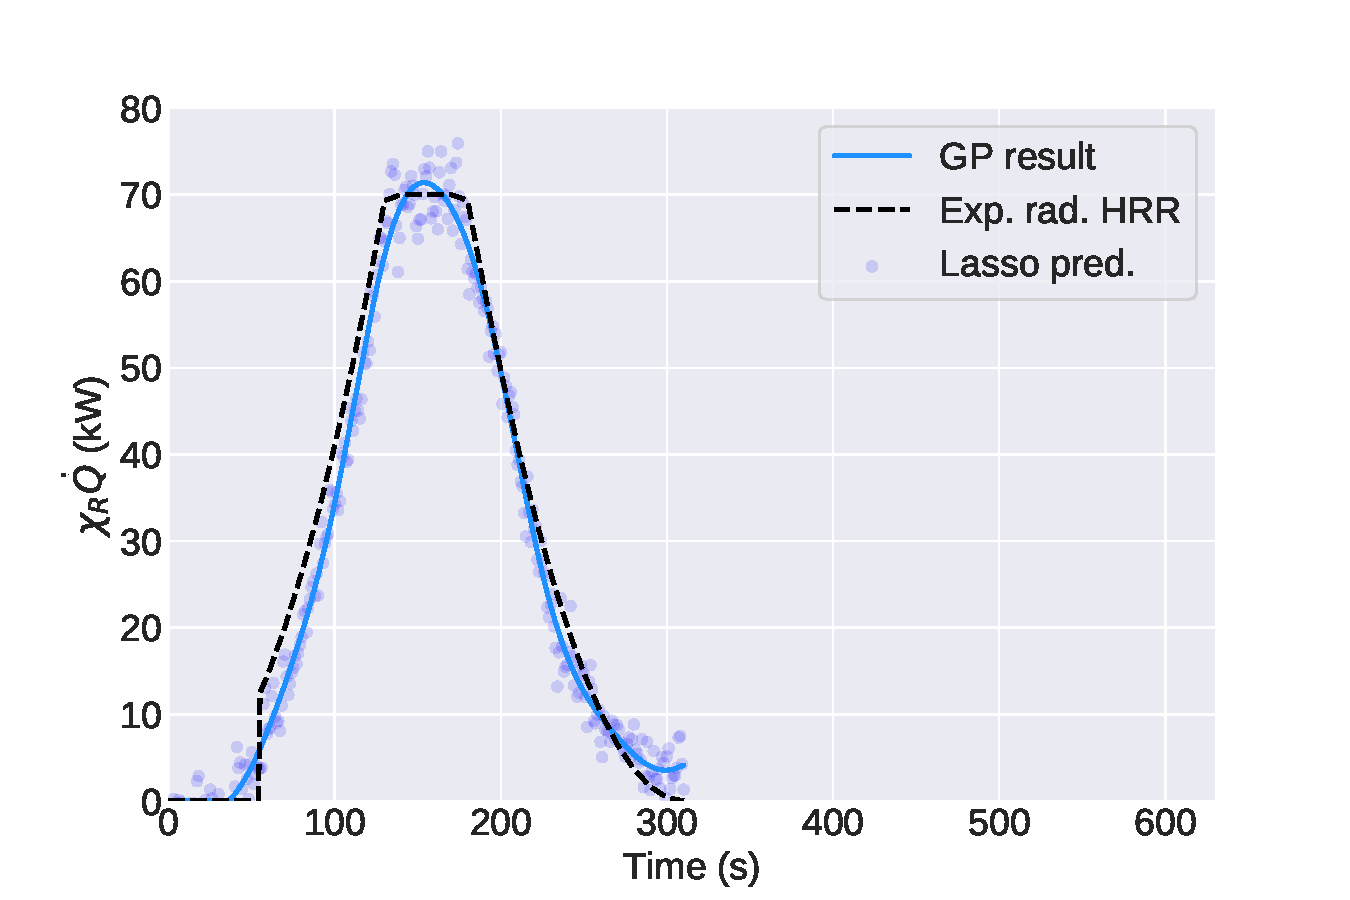
\includegraphics[width=\textwidth ,keepaspectratio]{figures/dft_result_t_squared.pdf}
      \caption{t-squared \\ MAE = 2.8 kW (9.5 \%)}
      \label{fig:dft_result_t_squared}
  \end{subfigure}
    \begin{subfigure}[t]{.45\textwidth}
      \centering
      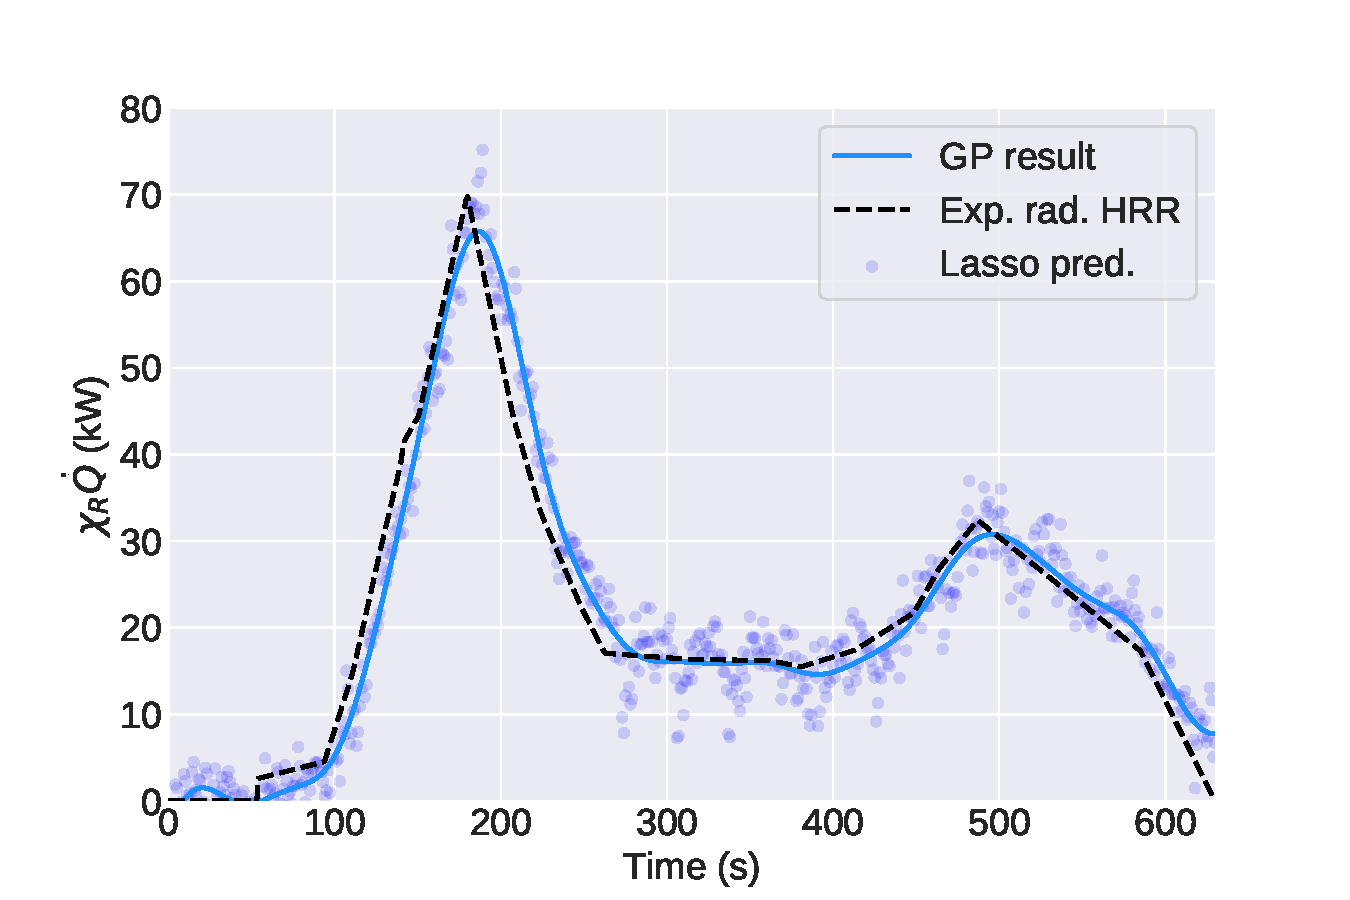
\includegraphics[width=\textwidth ,keepaspectratio]{figures/dft_result_weird_curve.pdf}
      \caption{Arbitrary ramp \\ MAE = 2.4 kW (11.2 \%)}
      \label{fig:dft_result_weird_curve}
  \end{subfigure}
  \caption{A demonstration of the methodology described in this section for each of the four burner experiments. For each experiment, the model trains on the other three experiments and predicts the radiative HRR ramp of the excluded experiment. Although the Lasso model produces noisy estimates, the Gaussian process regression is able to use the lasso predictions to make more accurate predictions.} 
  \label{fig:dft_gp_results}
\end{figure}



\clearpage
\subsection{Video analysis}
This section explores another machine learning approach for predicting the radiative heat release rate of a fire, which relies on analyzing video footage of the fire. The radiative heat release rate is specified because the approach is likely sensitive to the radiative fraction of the fuel burned. Nevertheless, this approach is likely the easiest to implement of the models described in the paper because it does not require any sensors besides a video camera and some method of producing fires with known HRR ramps for calibration. 

The central idea of this model is that the flame is expected to grow with increasing $\dot{Q}$. Using a video camera in a fixed location, a video of each burner experiment was collected. One frame was extracted as an image for every second of footage. The images were then reshaped into a 256 by 256 matrix of pixels. An example of these reshaped images is shown in Figure \ref{fig:fire_image}. Each pixel is described as a vector of length 3, with the entries describing the intensities of green, blue, and red light respectively on a scale from 0 to 255. In order to aggregate the three values into a single measure for each pixel, a ``normalized" intensity is calculated according to equation \ref{eqn:normalized_intensity},  

\begin{equation}
  \label{eqn:normalized_intensity}
 \text{Normalized intensity} = \frac{G + B + R}{(255)(3)}
\end{equation}

\noindent where $G$, $B$, and $R$ are the intensities of green, blue, and red light respectively. The denominator makes it so that the normalized intensity is on a scale between 0 and 1. Figure \ref{fig:brightness_heatmap} shows an example of a heatmap of the normalized intensity for an individual frame. Finally, a simple criterion is imposed to isolate the flame area. If the normalized intensity of a pixel is above 0.99, that pixel is assigned a value of 1; otherwise it is set to zero. Figure \ref{fig:binary_fire_image} shows the resulting binary map of this approach with the white region showing pixels that are above 99\% of the maximum normalized intensity and the black region showing all other pixels. 


\begin{figure}[htbp]
  \centering
  \begin{subfigure}[t]{.35\textwidth}
      \centering
      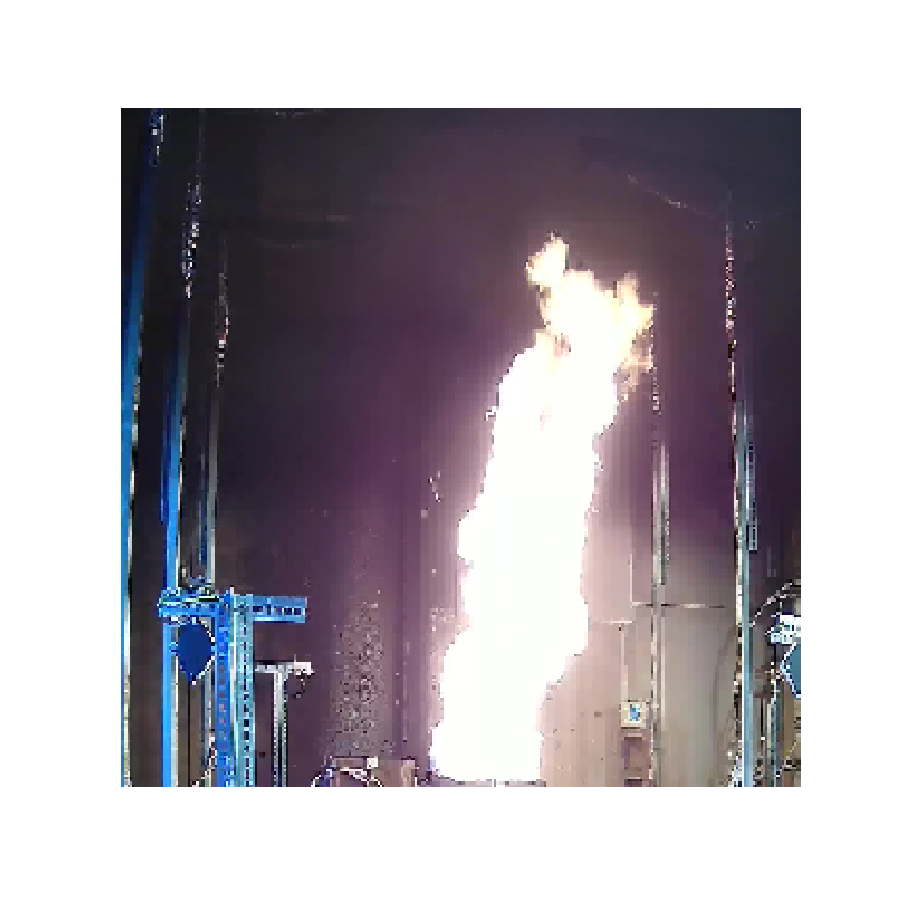
\includegraphics[width=\textwidth,keepaspectratio]{figures/fire_image.pdf}
      \caption{A resized (256x256) image of the fire from a frame of video footage.}
      \label{fig:fire_image}
  \end{subfigure}
  \begin{subfigure}[t]{.4\textwidth}
      \centering
      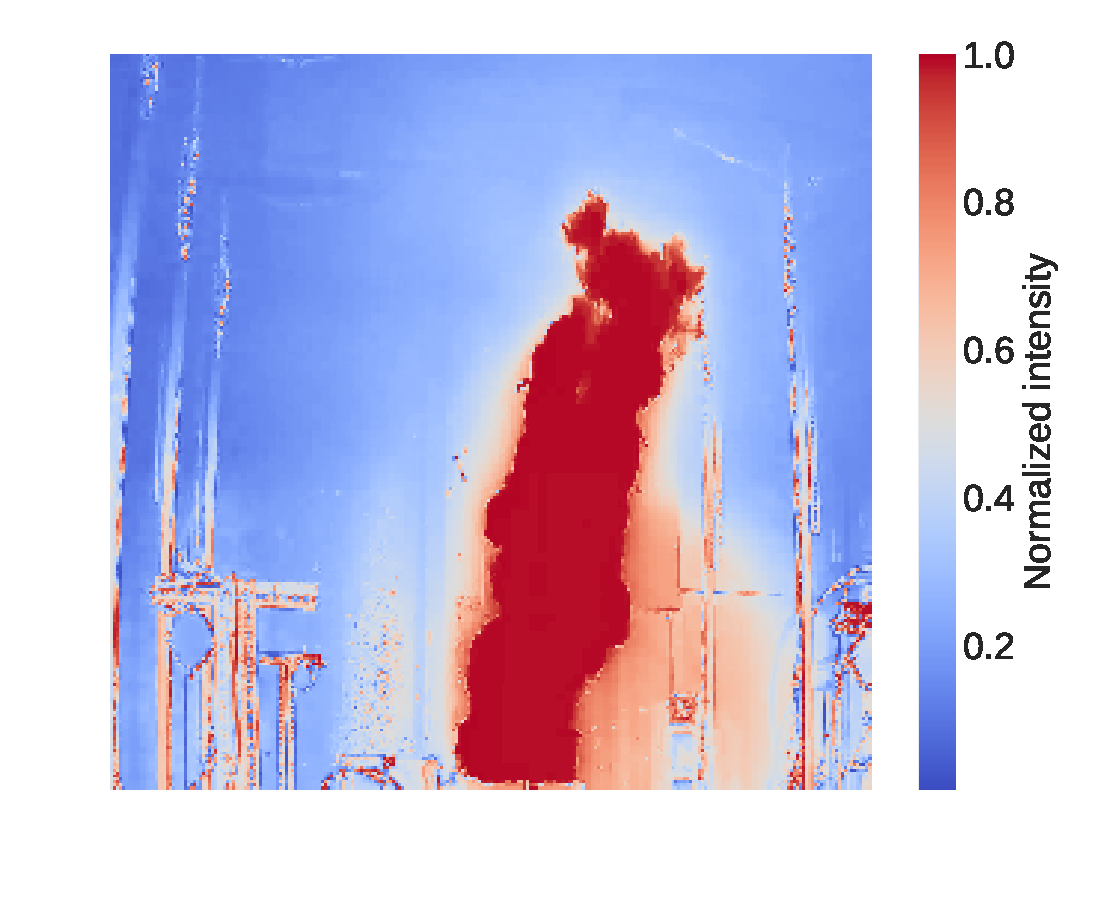
\includegraphics[width=\textwidth ,keepaspectratio]{figures/brightness_heatmap.pdf}
      \caption{Normalized intensity heatmap}
      \label{fig:brightness_heatmap}
  \end{subfigure}
  \begin{subfigure}[t]{.35\textwidth}
      \centering
      
\includegraphics[width=\textwidth ,keepaspectratio]{figures/binary_fire_image.pdf}
      \caption{Binary map identifying flame}
      \label{fig:binary_fire_image}
  \end{subfigure}
  \caption{Illustration of the video processing methodology. From the video, frames are extracted as 256x256 images such as the one shown in \protect\ref{fig:fire_image}. Each pixel has three intensity values which are aggregated into one value using equation \protect\ref{eqn:normalized_intensity} and this quantity is plotted as a heatmap in \protect\ref{fig:brightness_heatmap}. Finally, the pixels that have a normalized intensity above 0.99 are identified. These pixels are shown as white with all other pixels shown as black in \protect\ref{fig:binary_fire_image}.} 
  \label{fig:fire_image_processing}
\end{figure}

Next, the fraction, $f_{bright}$ of all pixels in the frame that are above 0.99 normalized intensity is computed. Figure \ref{fig:frac_bright} shows that the radiative heat release rate is correlated with this quantity, but there is non-linearity in the relationship. However, Figure \ref{fig:frac_bright_43} shows that $\dot{Q}_R = \chi_R\dot{Q}$ exhibits a fairly linear correlation with $f_{bright}^{4/3}$.


\begin{figure}[htbp]
  \centering
  \begin{subfigure}[t]{.45\textwidth}
      \centering
      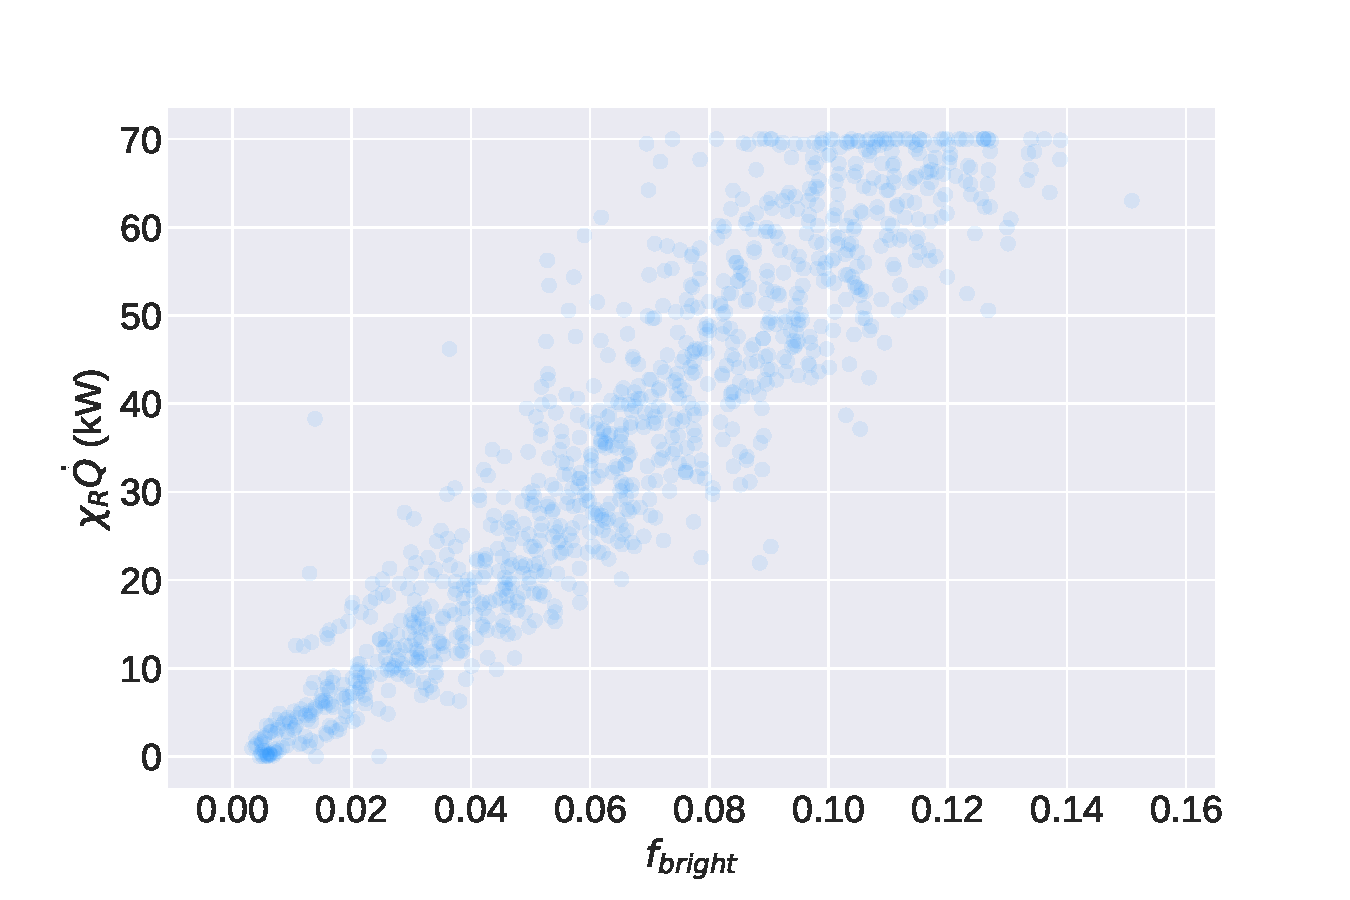
\includegraphics[width=\textwidth,keepaspectratio]{figures/frac_bright_scatterplot.pdf}
      \caption{}
      \label{fig:frac_bright}
  \end{subfigure}
  \begin{subfigure}[t]{.45\textwidth}
      \centering
      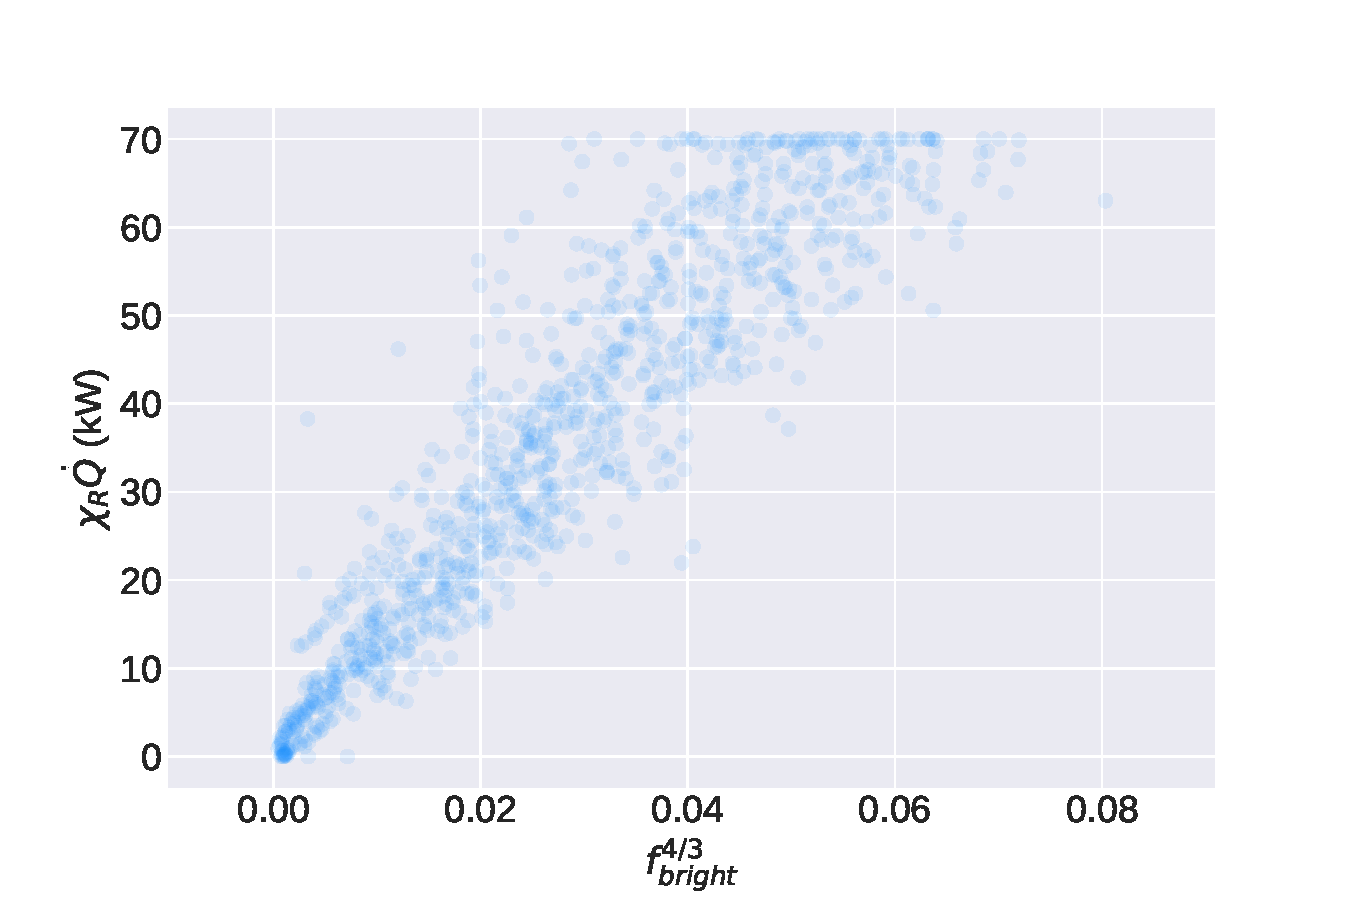
\includegraphics[width=\textwidth ,keepaspectratio]{figures/frac_bright_43_scatterplot.pdf}
      \caption{}
      \label{fig:frac_bright_43}
  \end{subfigure}
  \caption{Scatterplot showing the radiative heat release rate against the fraction of pixels with normalized intensities above 0.99 (\protect\ref{fig:frac_bright}). Raising $f_{bright}$ to the power of 4/3 appears to correct for the non-linearity in the relationship (\protect\ref{fig:frac_bright_43}).} 
  \label{fig:frac_bright_scatterplots}
\end{figure}


The linear correlation motivates the use of a simple linear regression, whose form is specified in equation 

\begin{equation}
  \label{eqn:bright_linear_regression}
 \dot{Q_R} = f_{bright}^{4/3}\beta
\end{equation}

The Gaussian process methodology described in the previous section is then repeated using the predictions from the simple regression model in place of the predictions from the lasso model with the heat flux measurements. The predictions of $\dot{Q}_R$ for each of the four experiments is shown in Figure \ref{fig:image_results}.

\begin{figure}[htbp]
  \centering
  \begin{subfigure}[t]{.45\textwidth}
      \centering
      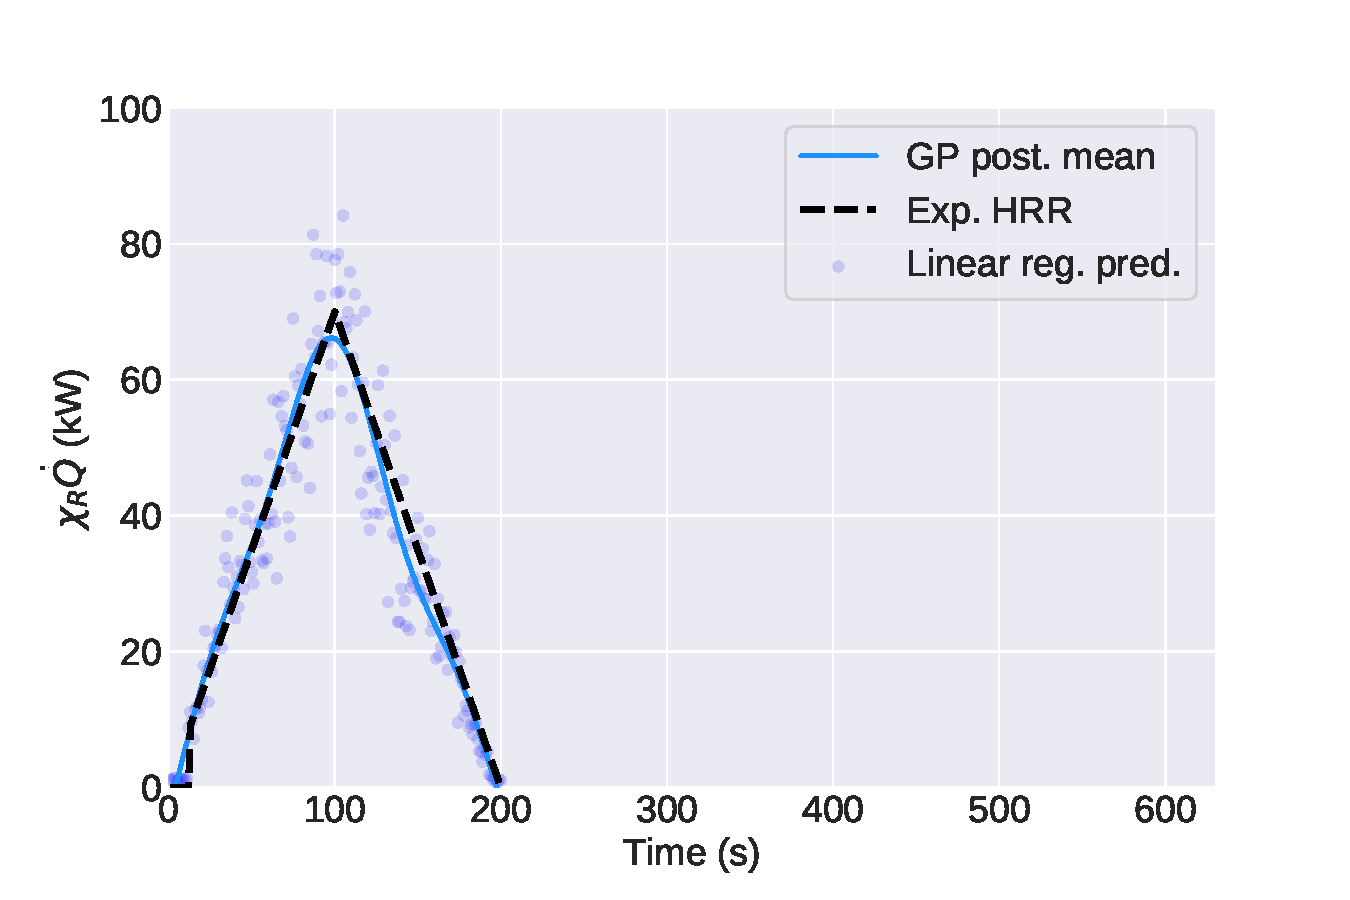
\includegraphics[width=\textwidth,keepaspectratio]{figures/image_result100s_triangle.pdf}
      \caption{100 second triangle \\ MAE = 2.2 kW (6.4 \%)}
      \label{fig:image_result_100s_triangle}
  \end{subfigure}
  \begin{subfigure}[t]{.45\textwidth}
      \centering
      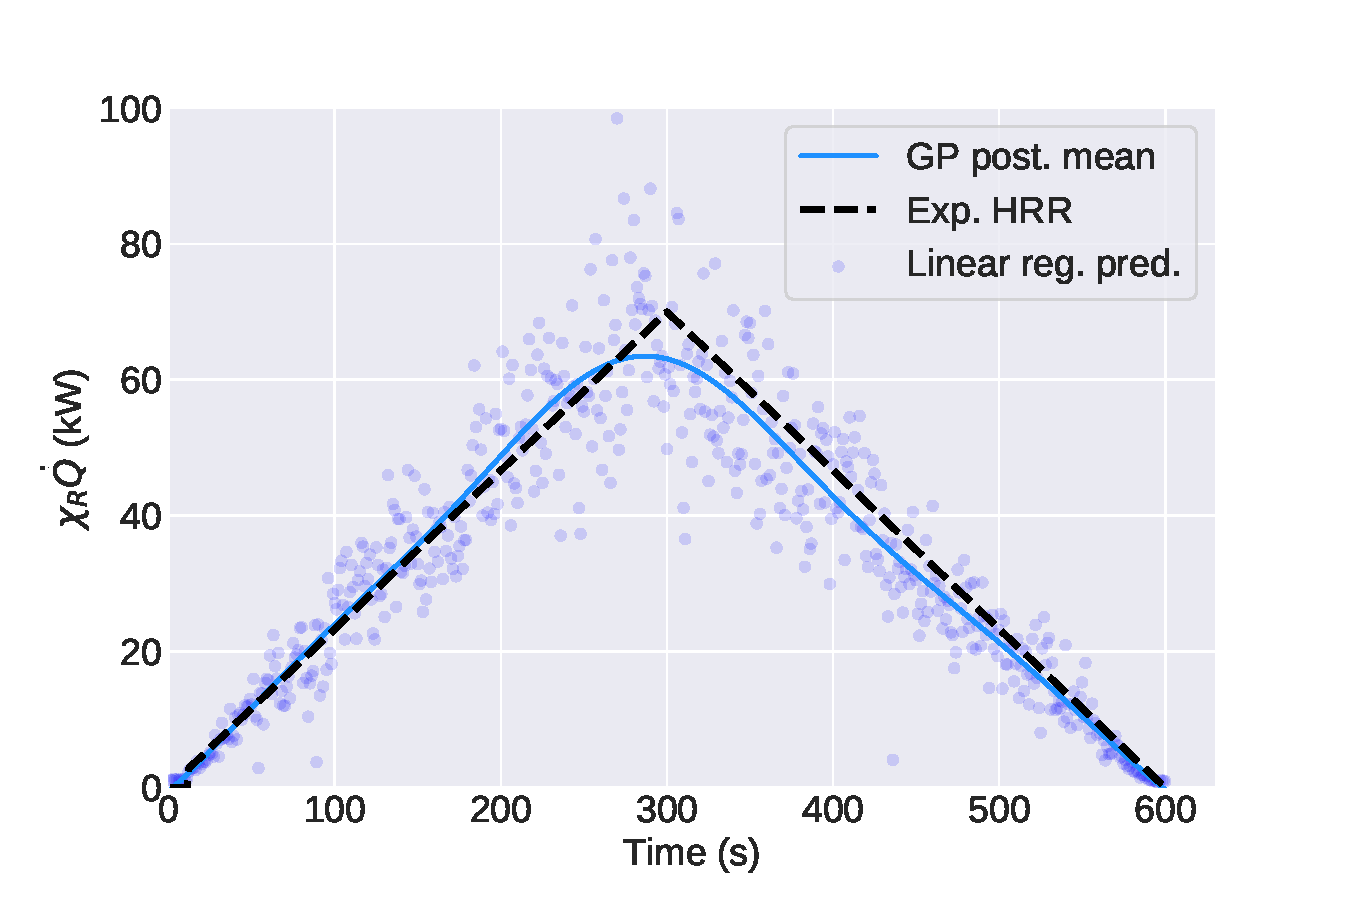
\includegraphics[width=\textwidth ,keepaspectratio]{figures/image_result300s_triangle.pdf}
      \caption{300 second triangle \\ MAE = 2.0 kW (5.8 \%)}
      \label{fig:image_result_300s_triangle}
  \end{subfigure}
   \begin{subfigure}[t]{.45\textwidth}
      \centering
      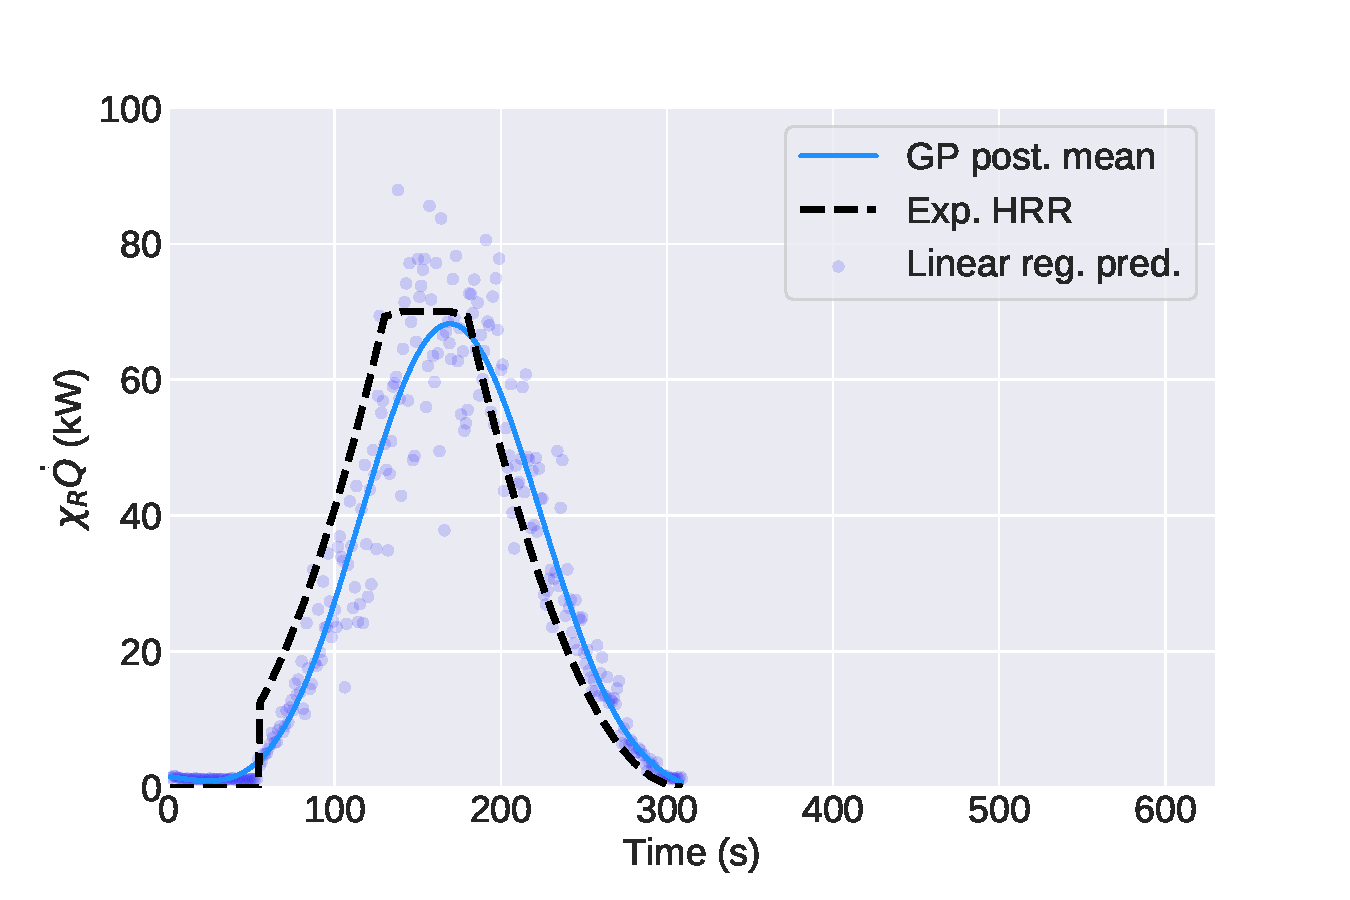
\includegraphics[width=\textwidth ,keepaspectratio]{figures/image_resultt_squared.pdf}
      \caption{t-squared \\ MAE = 6.8 kW (22.5 \%)}
      \label{fig:image_result_t_squared}
  \end{subfigure}
    \begin{subfigure}[t]{.45\textwidth}
      \centering
      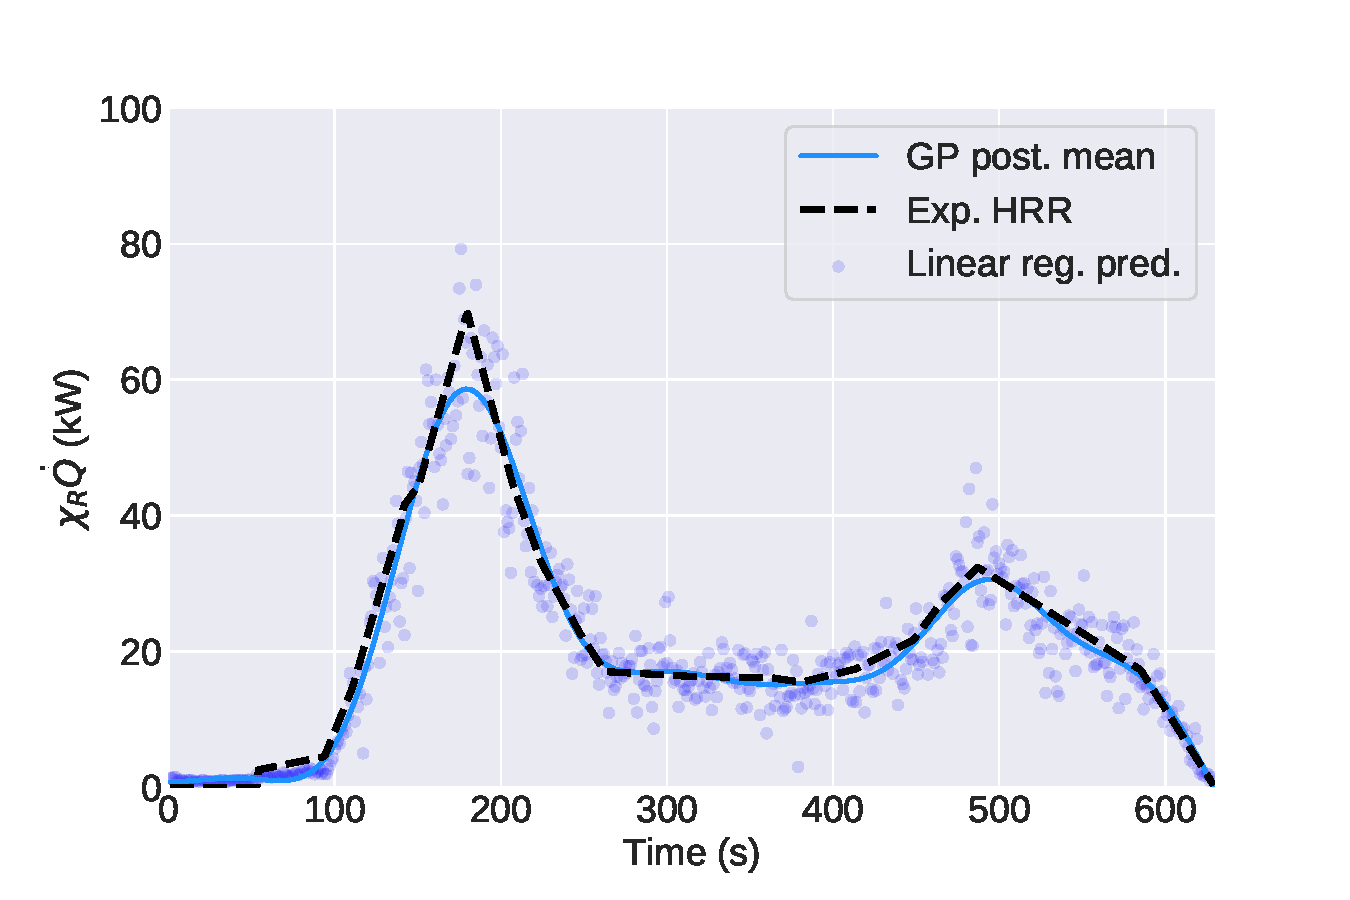
\includegraphics[width=\textwidth ,keepaspectratio]{figures/image_resultweird_curve.pdf}
      \caption{Arbitrary ramp \\ MAE = 1.4 kW (6.6 \%)}
      \label{fig:image_result_weird_curve}
  \end{subfigure}
  \caption{The predicted radiative HRR curve for each of the four burner experiments using the video analysis methodology described in this section. Again, for each of the four tests, the model is trained on the three other tests only.} 
  \label{fig:image_results}
\end{figure}

The results of this methodology appear to vary significantly across the four burner experiments. The linear regression predictions appear to be noisier than the lasso model used on the heat flux measurements, but interestingly the Gaussian process predicts the radiative HRR more accurately than its counterpart described in the previous section, at least for the triangle fires and the arbitrary ramp fire. The predictions in the t-squared fire appear to lag behind the actual radiative HRR, though it is not clear why. The burner ignited the latest in this experiment of the four (~50 seconds), but one would expect that a framework based on video analysis would not exhibit time lag effects. 


\clearpage
\subsection{Thermocouple measurements}
In this section, various models are presented for predicting the heat release rate of a fire based on a set of thermocouple measurements. The models presented in the previous sections are assumed to depend signficantly on the radiative fraction, $\chi_R$ of the fuel, and therefore are assumed to provide insight into the the radiative component of the heat release rate, $\chi_R$, rather than the total heat release rate, $\dot{Q}$. Ideally, the temperatures can provide information on $\dot{Q}_R$ regardless of $\chi_R$, making the calorimetry framework robust to differences in fuels. To examine if this is the case, a sensitivity analysis was conducted to examine how much varying $\chi_R$ affects the thermocouple responses. This was done by running 10 different FDS cases modeling the experimental setup. For all cases, the total HRR ramp was a symmetric triangle fire with a peak HRR of 200 kW and a 200 second time to peak. However, $\chi_R$ was varied from 0 to 0.40 in the simulations. The results are shown in Figure \ref{fig:constant_Qtot_assumption}. 

\begin{figure}[htb] \centering
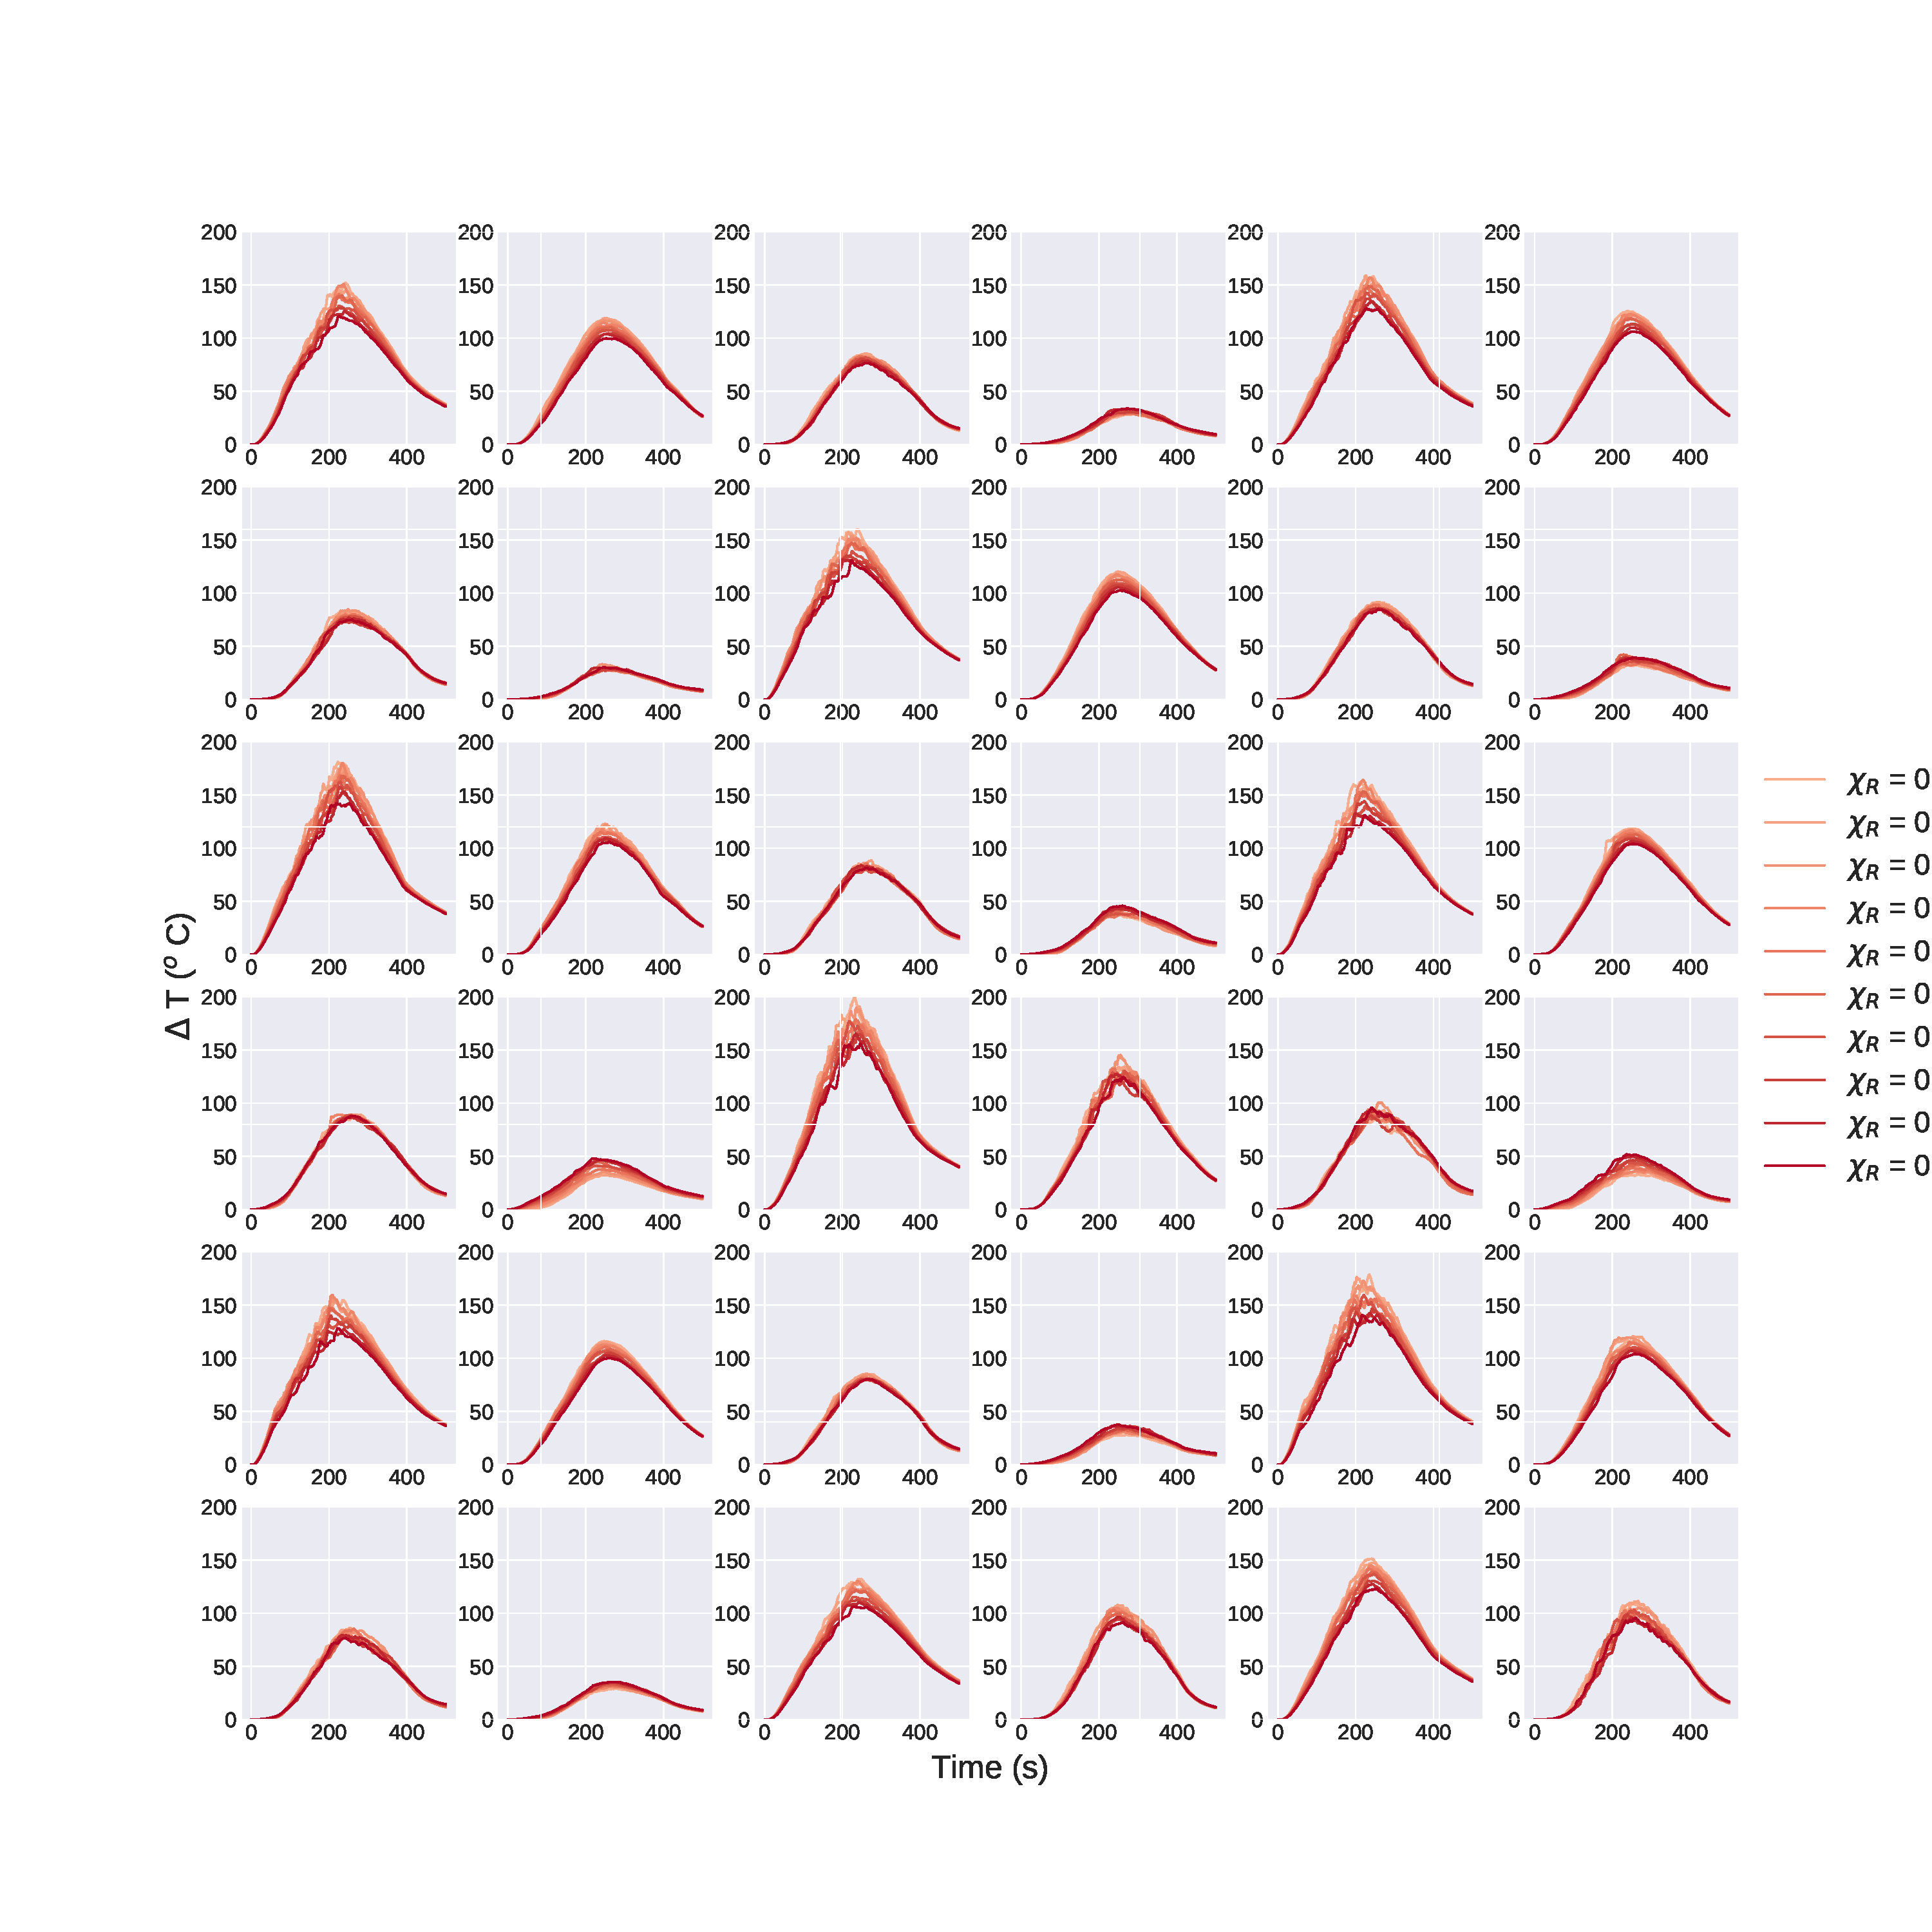
\includegraphics[width=.9\textwidth]{./figures/constant_Qtot_assumption.pdf}
\caption{A matrix of plots showing the sensitivity of the predicted thermocouple response to different radiative fractions, $\chi_R$. 10 different FDS cases were run and the total HRR ramp was the same across all cases; however, the radiative fraction was varied from $\chi_R = 0$ to $\chi_R=0.4$. The total HRR ramp for all cases is a symmetric triangle fire with a peak HRR of 200 kW that reaches the peak in 200 seconds.}
\label{fig:constant_Qtot_assumption}
\end{figure}

The results indicate that the thermocouple responses are relatively insensitive to $\chi_R$. This is likely due to the fact that the thermocouples are heated from both convection and radiation, so when the total heat output from the fire is the same, they will experience a similar amount of heating irrespective of the contributions of the individual heat transfer modes. 

The next step is to explore the relationship between the temperature differences, $\Delta T$ measured by the thermocouples and $\dot{Q}$. A scatterplot such as the one shown in Figure \ref{fig:temp_scatter} serves as a useful starting point.  


\begin{figure}[htb] \centering
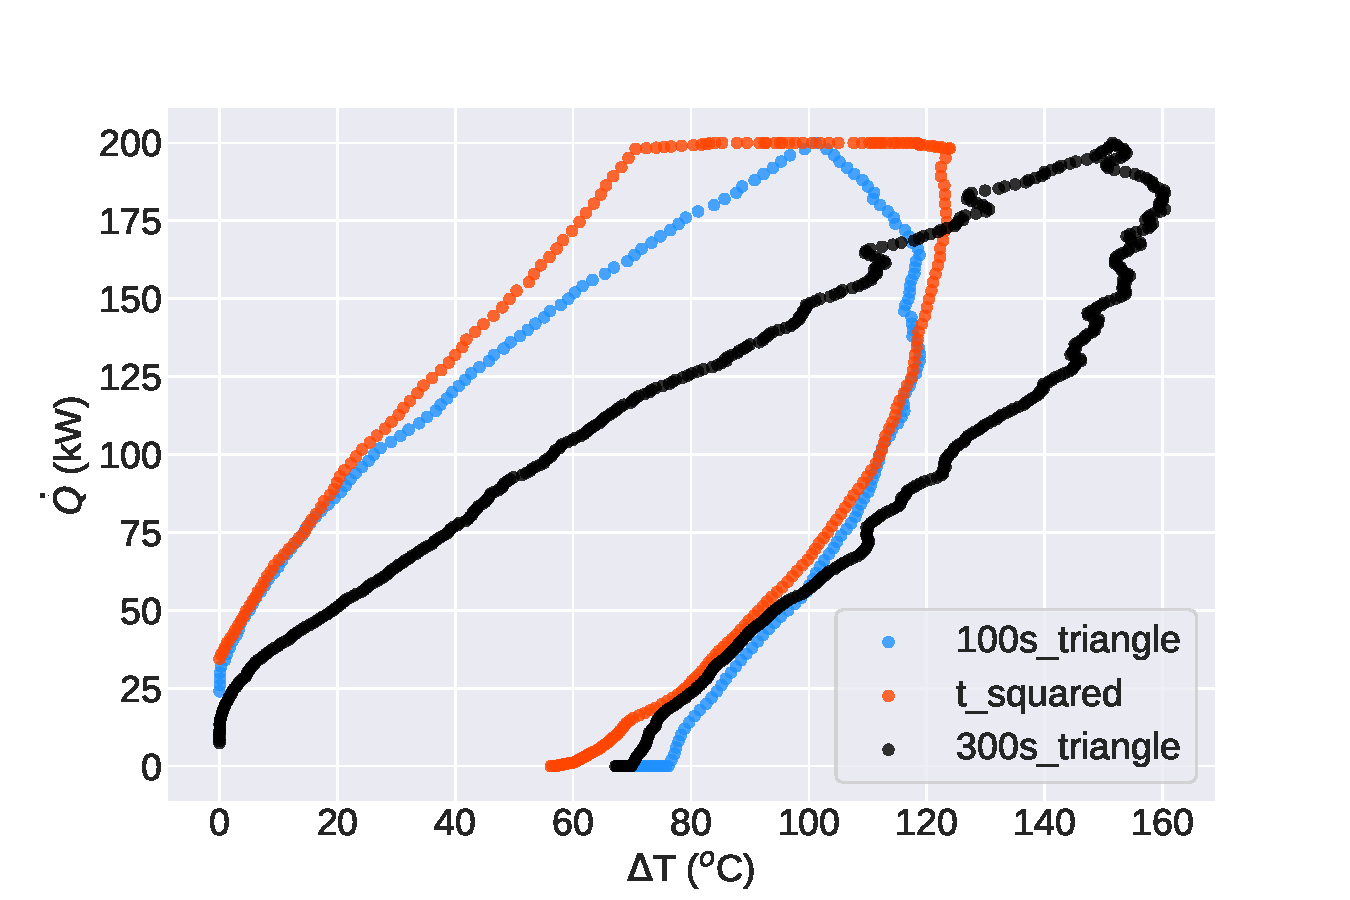
\includegraphics[width=.75\textwidth]{./figures/temp_scatter.pdf}
\caption{A scatterplot of the total heat release rate, $\dot{Q}$ vs. the experimentally measured $\Delta T$ of a single thermocouple. The result is typical of all other thermocouples and shows that the temperature response exhibits complex hysteresis that hinders the effectiveness of standard regression models. }
\label{fig:temp_scatter}
\end{figure}

Although the results shown in Figure \ref{fig:temp_scatter} are from only one of the 35 thermocouples that collected measurements during the experiments, the results are representative of the other sensors. Unlike the heat flux measurements, which show a linear relationship with $\dot{Q}$, the thermocouple measurements are characterized by complicated hysteretic paths that greatly hinder the use of ordinary statistical models. This is expected given the fact that the thermal masses of thermocouples make their measurements dependent on the history of surrounding gas temperatures and radiative heat fluxes. Furthermore, the surrounding gas temperature is also dependent on the fire's HRR history, meaning that the HRR cannot be reasonably inferred using only thermocouple measurements at an instant in time. These results motivate the use of physical models, which can predict a thermocouple's response as a time series given an HRR time series. FDS has this capability, but the simulations are computationally expensive and a HRR inversion framework can require many runs. The speed of the runs can be greatly improved by using coarser meshes at the potential expense of accuracy. In order to gain insight into which thermocouples are ideal for HRR inversion, two FDS simulations were run of the previously described 200 second triangle fire. In one simulation, the cells are 20 cm by 20 cm by 10 cm, and in the other they are 10 cm by 10 cm by 5 cm. The former case runs approximately eight times faster, but it is a relatively coarse mesh and may not full resolve the flow in some regions. Figure \ref{fig:grid_sensitivity} shows the results of these FDS simulations for the thermocouple locations used in the experiments.


\begin{figure}[htbp]
  \centering
  \begin{subfigure}[t]{.45\textwidth}
      \centering
      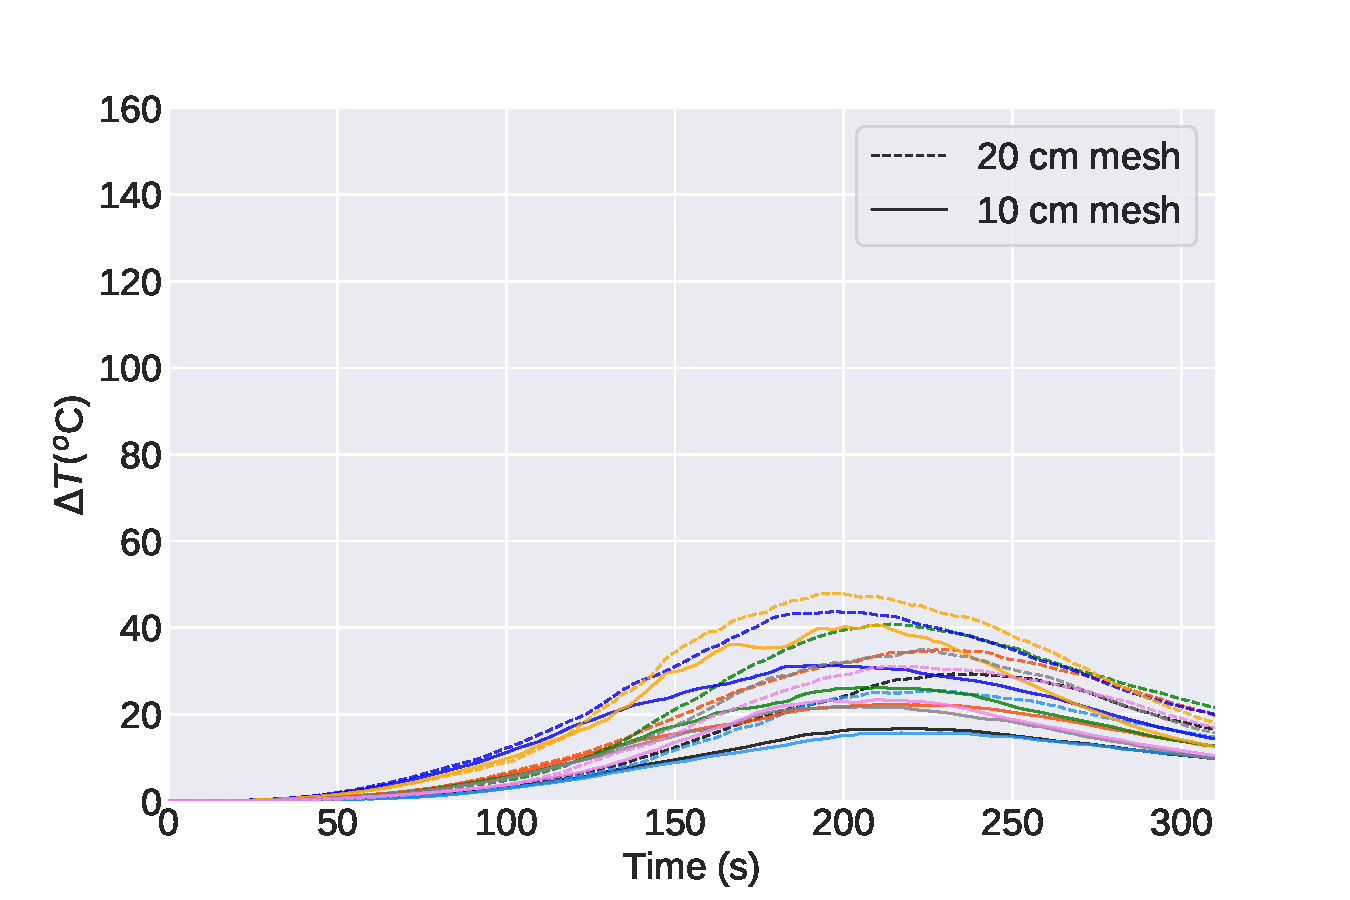
\includegraphics[width=\textwidth,keepaspectratio]{figures/053mesh_sensitivity.pdf}
      \caption{0.53 m off ground}
      \label{fig:0.53mesh_sensitivity}
  \end{subfigure}
  \begin{subfigure}[t]{.45\textwidth}
      \centering
      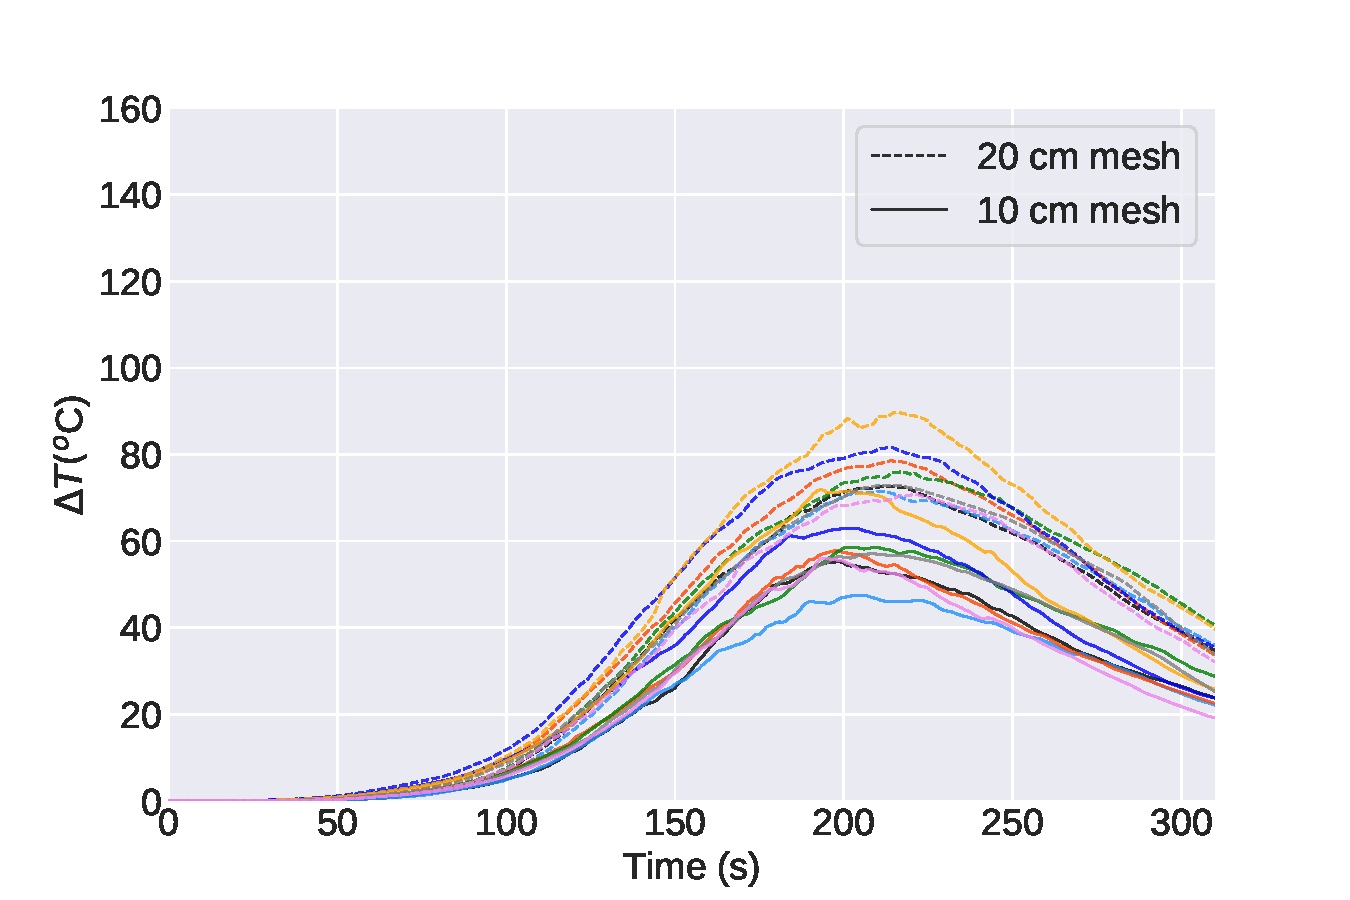
\includegraphics[width=\textwidth ,keepaspectratio]{figures/107mesh_sensitivity.pdf}
      \caption{1.07 m off ground}
      \label{fig:1.07mesh_sensitivity}
  \end{subfigure}
   \begin{subfigure}[t]{.45\textwidth}
      \centering
      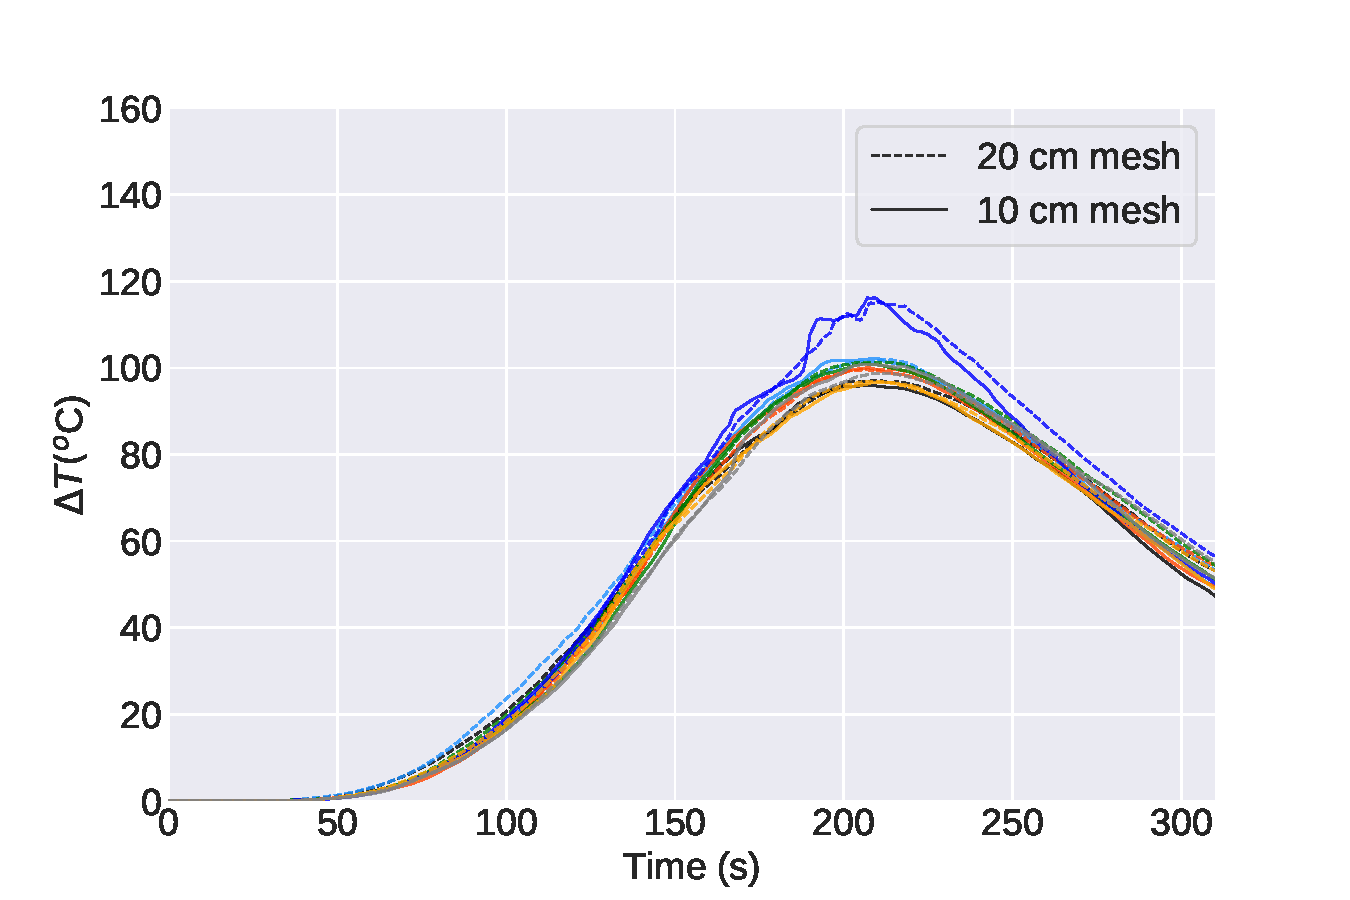
\includegraphics[width=\textwidth ,keepaspectratio]{figures/16mesh_sensitivity.pdf}
      \caption{1.6 m off ground}
      \label{fig:1.6mesh_sensitivity}
  \end{subfigure}
    \begin{subfigure}[t]{.45\textwidth}
      \centering
      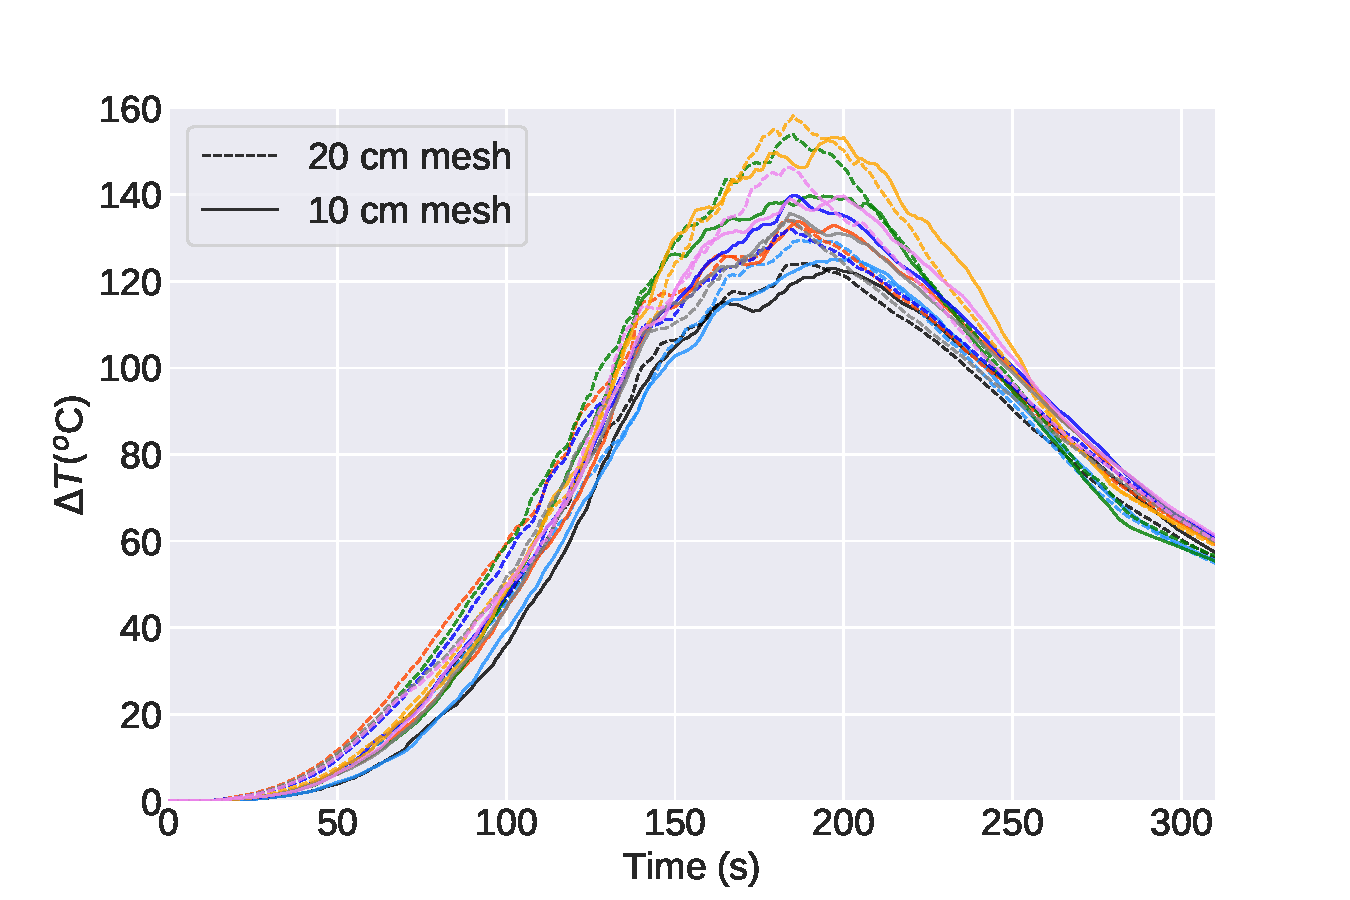
\includegraphics[width=\textwidth ,keepaspectratio]{figures/211mesh_sensitivity.pdf}
      \caption{2.1 m off ground}
      \label{fig:2.11mesh_sensitivity}
  \end{subfigure}
  \caption{The simulated responses of all thermocouples in the experiment using both a 10 cm x 10 cm x 5 cm mesh and a 20 cm x 20 cm x 10 cm mesh. The HRR ramp is the 100 second triangle fire previously described. The thermocouples are grouped by their heights off the ground. The results indicate that the thermocouples higher off the ground are both more sensitive to the HRR and less sensitive to the grid size, making them ideal for the HRR inversion framework.}
  \label{fig:grid_sensitivity}
\end{figure}


The ideal thermocouples are the ones whose measurements are the most sensitive to the quantity of interest, $\dot{Q}$, and the least sensitive to the use of a coarse mesh in FDS. Notice that the thermocouples that are 1.6 m off the ground or higher exhibit both of these figures of merit. As a result, these 17 thermocouples are used for the HRR inversion framework. 


\clearpage
\subsubsection{Forward FDS emulators}

Even with the coarse mesh, the FDS simulations can still be computationally expensive, taking nearly 30 minutes to run for one simulation, and many simulations can be required for inverse problems. Ideally, the inversion framework could provide nearly instantaneous estimates of the HRR using data collected from a new experiment without sacrificing accuracy. One way to accomplish this is to use emulators of FDS. These are machine learning models that learn the mapping between the input and the output of a physical model in order to circumvent the need for additional simulations. Specifically, an array of of artifical neural networks (ANN) is used to learn the mapping between a transient HRR $\dot{Q}(t)$ and an array of transient thermocouple responses, $\begin{bmatrix} \Delta T_1(t) & \Delta T_2(t) & \ldots & \Delta T_{17}(t) \end{bmatrix}$. A schematic of an emulator ANN is shown in Figure \ref{fig:neural_network_drawings} for a single thermocouple. 

\begin{figure}[htbp]
  \centering
  \begin{subfigure}[t]{.6\textwidth}
      \centering
      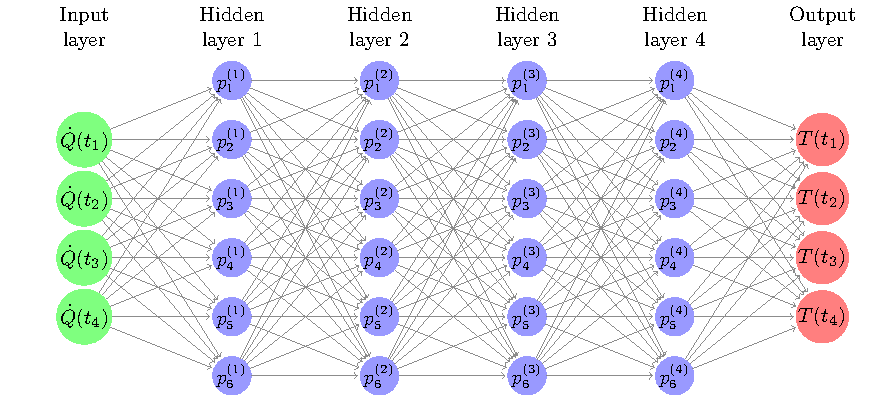
\includegraphics[width=\textwidth,keepaspectratio]{figures/neural_netowrk_diagram.pdf}
      \caption{A simplified diagram of the neural network   }
      \label{fig:neural_network_diagram}
  \end{subfigure}
  \begin{subfigure}[t]{.35\textwidth}
      \centering
      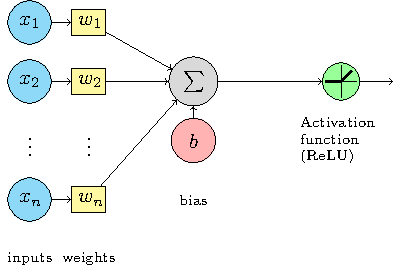
\includegraphics[width=\textwidth ,keepaspectratio]{figures/perceptron_diagram.pdf}
      \caption{}
      \label{fig:perceptron_diagram}
  \end{subfigure}
  \caption{\protect\ref{fig:neural_network_diagram} shows a simplified diagram of the neural network architecture used for each thermocouple response. In reality, the input layer and output layers each have 91 nodes as opposed to four, and each of the hidden layers has 128 perceptrons as opposed to six. The neural network is fully connected, meaning that each output of a given layer is an input to every perceptron in the next layer. \protect\ref{fig:perceptron_diagram} is a diagram showing the operation of an individual perceptron. All of the inputs to a given perceptron are weighted and then summed with an additional bias parameter. The result of this summation is sent through an activation function, which is the rectified linear activation function (ReLU) with the exception of the output layer, which simply outputs the sum.} 
  \label{fig:neural_network_drawings}
\end{figure}



Both the HRR time series, $\dot{Q}(t)$, and the thermocouple response time series, $\Delta T (t)$, are discretized into 91 evenly spaced points over the interval [0, 900] seconds. In other words, the ANN learns the mapping between the vectors $\dot{Q}(\boldsymbol{t})$ and $\Delta T_i(\boldsymbol{t})$ where $\boldsymbol{t} = \boldsymbol{t}^{\text{NN}}  =  \begin{bmatrix} 0 & 10 & \ldots & 900 \end{bmatrix}$ seconds. Figure \ref{fig:neural_network_diagram} is a diagram of an ANN for an individual thermocouple response. Each of the entries in $\dot{Q}(\boldsymbol{t})$ is passed to each of the 128 perceptrons in the first hidden layer. A diagram of an individual perception is shown in Figure \ref{fig:perceptron_diagram}.  The perceptron computes a weighted sum of all inputs and adds a bias. The result of this summation is passed through a recitified linear activation function, which returns the result if it is positive and returns zero otherwise. The output of the activation function then becomes an input to every perceptron in the next layer. A linear activation function is used in the output layer, which means that these perceptrons simply return the weighted sum of their inputs and their bias. Each perceptron in the first hidden layer has 92 parameters to learn (91 weights plus one bias) and all other perceptrons have 129 parameters to learn (128 weights plus one bias). This totals to 73,051 trainable parameters. The ANNs are constructed using the sequential method in the Python package Keras \cite{chollet2018keras}. The parameters are trained using the Adam method \cite{kingma2014adam}, which is a stochastic optimization method. The batch size is set to 31, the validation split is  20\% of the data. Also, the authors found that the performance is improved by dividing $\dot{Q}(t)$ by 200 kW and $\Delta T(t)$ by 200 $^oC$. This normalization makes it so that the inputs and outputs will generally vary on the order of one, which can lead to improved training \cite{sola1997importance}. 

The next consideration is how to build a training set for the emulators. Using the previously discussed Gaussian process framework, a random distribution of viable HRR curves is specified, $\dot{Q}(t)\sim \mathcal{GP}(m,K)$, where $\dot{Q}_{max} =$. In the previous sections, the prior mean function was set to zero for simplicity and because the posterior GP is strongly informed by the data, so the prior mean has little impact. In the current case, the mean function has a significant impact on the family of functions drawn from the GP. If the mean is zero, them the function evaluations are equally likely to be positive or negative (like the draws shown in \ref{fig:gp_prior}), which is not ideal for constructing HRR curves given that the HRR must be positive. Because of this, the mean function, $m(t)$, is set to  a constant 150 kW which gives the GP a tendency to favor positive function evaluations.  The squared exponential kernel function (equation \ref{eqn:squared_exponential}) is used again here. The hyperparameters, $\tau$ and $b$, were previously determined through a statistical optimization process. Here, they are chosen less formally with the goal of producing a reasonable distribution of HRR curves. Future work should explore the optimal hyperparameters and kernel functions for maximizing the training efficiency of the emulators. Nevertheless, the approach outlined here appears to produce reasonably good results. The hyperparameter, $\tau^2$ is chosen to be 8,100 kW$^{\text{2}}$, meaning that the standard deviation of any individual function evaluation is $\sqrt{8100} = 90$ kW, producing a reasonable variation of HRR values centered around 150 kW. For some cases, a bandwidth, $b$, of 30 seconds was used and for other cases, a bandwidth of 60 seconds was used based on visual inspection of the results. Another important consideration is that the functions must start at $\dot{Q}(0) = 0$ and end at $\dot{Q}(t_{end}) = 0$. One approach would be to change the corresponding values of the drawn functions to zero, but this can result in sharp discontinuities that are unphysical. Instead, the initial and end conditions can be imposed in the Gaussian process itself, producing random functions that ``gracefully" start and end at zero. This can be done using the previously described Bayesian updating approach, treating the start and end conditions as observations with zero unceratinty (i.e. $\sigma^2 = 0$). Let $\boldsymbol{t}^{\text{zero}} = \begin{bmatrix} 0 & t_{end}  \end{bmatrix}$ be a vector of times at which $Q(t)$ is zero, i.e. $Q(\boldsymbol{t}^{\text{zero}}) = \boldsymbol{0}$. The objective is to evaluate a distribution of function evaluations, $p\Big(\dot{Q}(\boldsymbol{t}^{\text{NN}})\Big)$ for functions that satisfy this constraint. Similar to equation \ref{eqn:joint_GP}, the joint distribution is shown in equation \ref{eqn:joint_hrr_gp}.


\begin{equation}
  \label{eqn:joint_hrr_gp}
  \begin{bmatrix}
  \dot{Q}(\boldsymbol{t}^{\text{zero}}) \\
  \dot{Q}(\boldsymbol{t}^{\text{NN}})
  \end{bmatrix} \sim 
  \mathcal{N} \Bigg( \begin{bmatrix}
  m(\boldsymbol{t}^{\text{zero}}) \\
  m(\boldsymbol{t}^{\text{NN}})      
  \end{bmatrix}  \ \ \ 
  \begin{bmatrix}
 K(\boldsymbol{t}^{\text{zero}}, \boldsymbol{t}^{\text{zero}}) & K(\boldsymbol{t}^{\text{zero}}, \boldsymbol{t}^{\text{NN}}) \\ 
   K(\boldsymbol{t}^{\text{NN}}, \boldsymbol{t}^{\text{zero}}) &  K(\boldsymbol{t}^{\text{NN}}, \boldsymbol{t}^{\text{NN}}) 
  \end{bmatrix}
  \Bigg)
\end{equation}

\noindent Note that the mean vector is no longer a vector of zeros as it was in equation \ref{eqn:joint_GP}.  Instead, it is written in terms of the mean function, which returns a vector in which all entries are 150 kW. Again, Bayes' law is applied to give the result shown in equation \ref{eqn:hrr_train_posterior}.

\begin{equation}
  \label{eqn:hrr_train_posterior}
 \dot{Q}(\boldsymbol{t}^{\text{NN}})  \Big| \dot{Q}(\boldsymbol{t}^{\text{zero}}) \sim 
 \mathcal{N}\Big(\boldsymbol{m}_{post}, \boldsymbol{C}_{post}\Big)
\end{equation}

\noindent where 

$$
\boldsymbol{m}_{post} = 
m(\boldsymbol{t}^{\text{NN}}) -  K(\boldsymbol{t}^{\text{NN}}, \boldsymbol{t}^{\text{zero}})\Big[K(\boldsymbol{t}^{\text{zero}}, \boldsymbol{t}^{\text{zero}}) \Big]^{-1} m(\boldsymbol{t}^{\text{zero}})
$$

\noindent and 

$$
\boldsymbol{C}_{post} = K(\boldsymbol{t}^{\text{NN}}, \boldsymbol{t}^{\text{NN}}) -  K( \boldsymbol{t}^{\text{NN}}, \boldsymbol{t}^{\text{zero}})\Big[K(\boldsymbol{t}^{\text{zero}}, \boldsymbol{t}^{\text{zero}})\Big]^{-1}K(\boldsymbol{t}^{\text{zero}},\boldsymbol{t}^{\text{NN}})
$$


The expressions for the mean and covariance are slightly different than in equation \ref{eqn:gp_posterior} because of the non-zero mean vector. Also, the observed function evaluations, $\dot{Q}(\boldsymbol{t}^{\text{zero}})$ (analagous to $\dot{Q}_{R}^{\text{lasso}}(\boldsymbol{t}^{\text{DFT}})$ in equation \ref{eqn:gp_posterior}) are a vector of zeros with zero variance ($\sigma^2=0)$. As a result $\dot{Q}(\boldsymbol{t}^{\text{zero}})$ does not appear in the expression for $\boldsymbol{m}_{post}$. A final consideration is that the emulators should be able to produce the results from FDS simulations of variable duration. As a result, the duration of the simulation, $t_{end}$ is uniformly drawn between 150 and 900 seconds. For each drawn HRR curve, $t_end$ is drawn first, which determines $\boldsymbol{t}^{\text{zero}}$. Then a HRR curve is drawn according to the distribution described by equation \ref{eqn:hrr_train_posterior}. The times at which the drawn functions are evaluated, $\boldsymbol{t}_{NN}$ is identical regardless of the drawn $t_{end}$. However, $\dot{Q}(t_i^{\text{NN}})$ is set to zero if $t^{\text{NN}}_i > t_{end}$.

Examples of HRR curves randomly generated from this approach are shown in Figure \ref{fig:gp_nn_training}. 

\begin{figure}[htbp]
  \centering
  \begin{subfigure}[t]{.45\textwidth}
      \centering
      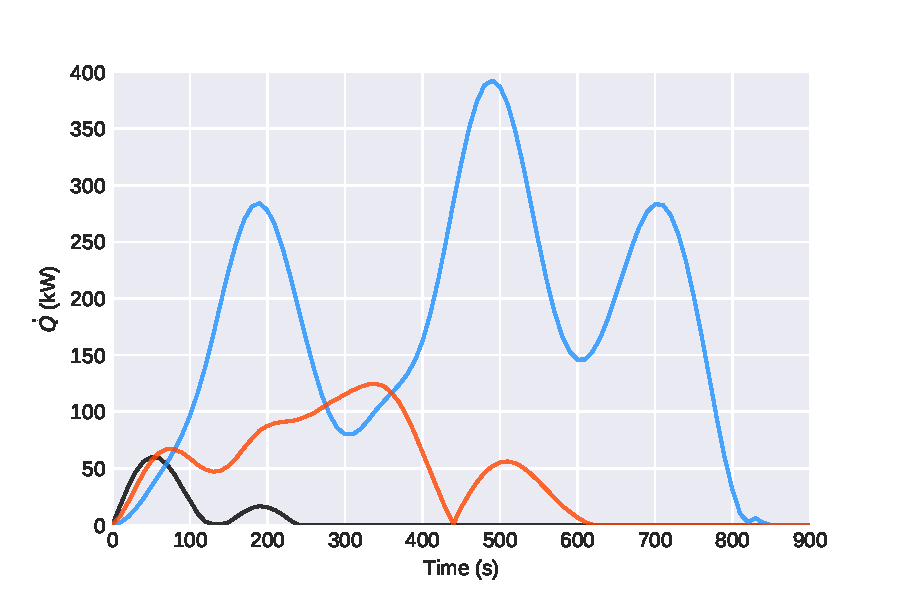
\includegraphics[width=\textwidth,keepaspectratio]{figures/gp_nn_training_smooth.pdf}
      \caption{ $b=60$ sec.}
      \label{fig:gp_nn_training_smooth}
  \end{subfigure}
  \begin{subfigure}[t]{.45\textwidth}
      \centering
      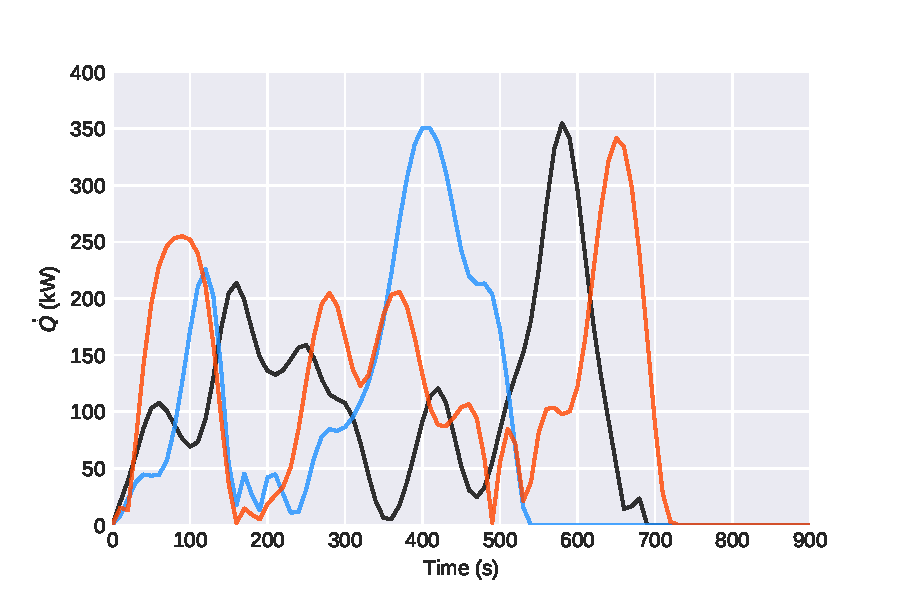
\includegraphics[width=\textwidth ,keepaspectratio]{figures/gp_nn_training_wiggly.pdf}
      \caption{ $b=30$ sec.}
      \label{fig:gp_nn_training_wiggly}
  \end{subfigure}
  \caption{Example draws from the Gaussian processes used to generate the random HRR curves in the neural network training set. \protect\ref{fig:gp_nn_training_smooth} shows that the drawn functions are smoother when the bandwidth is set to 60 seconds compared to those shown in \protect\ref{fig:gp_nn_training_wiggly} using a bandwidth of 30 seconds. The emulators train on functions drawn from both distributions. Note that the HRR curves also have a varying duration so that the emulators can learn to produce the results from FDS simulations with different simulation durations.} 
  \label{fig:gp_nn_training}
\end{figure}

A major drawback of using ANNs to emulate FDS simulations is that they must train on a large number of examples before they achieve reasonable accuracy. However, it was found that utilizing transfer learning can dramatically reduce the number of runs required to achieve a small amount of error. Transfer learning refers to the concept of training neural networks to perform a similar task before training them to perform the task of interest. Specifically, the task of predicting the response of a thermocouple in FDS is similar to the task of predicting the upper gas layer response in a two-zone fire model, such as the Consolidated Model of Fire and Smoke Transport (CFAST) \cite{peacock1993cfast}, developed by NIST. This is a simplified model of a fire which divides the compartment into two zones: an upper layer and a lower layer and conservation equations are solved for the two zones. This approach leads to simulations that run orders of magnitude faster than FDS, but are generally less accurate and have less spatial resolution. 

When an ANN is initialized, its parameters are generally set to random values. If the parameters are initialized to values that are closer to the optimal set of values, then the ANN can learn to predict FDS outputs with fewer training examples. Using the previously described method of generating random HRR curves, 20,000 simulations of CFAST were run based on the experimental burn structure. Because of the simplified physics, 20,000 simulations can be generated from CFAST in about an hour without parallelization. An ANN is then trained to predict the simulated temperature of the upper layer as a function of time. When the first ANN is trained to predict a thermocouple response in FDS, its weights and biases are initialized to those of the ANN trained to predict the CFAST upper layer temperature. This process greatly accelerates the training process, as shown in Figure \ref{fig:transfer_learning}. 


\begin{figure}[htb] \centering
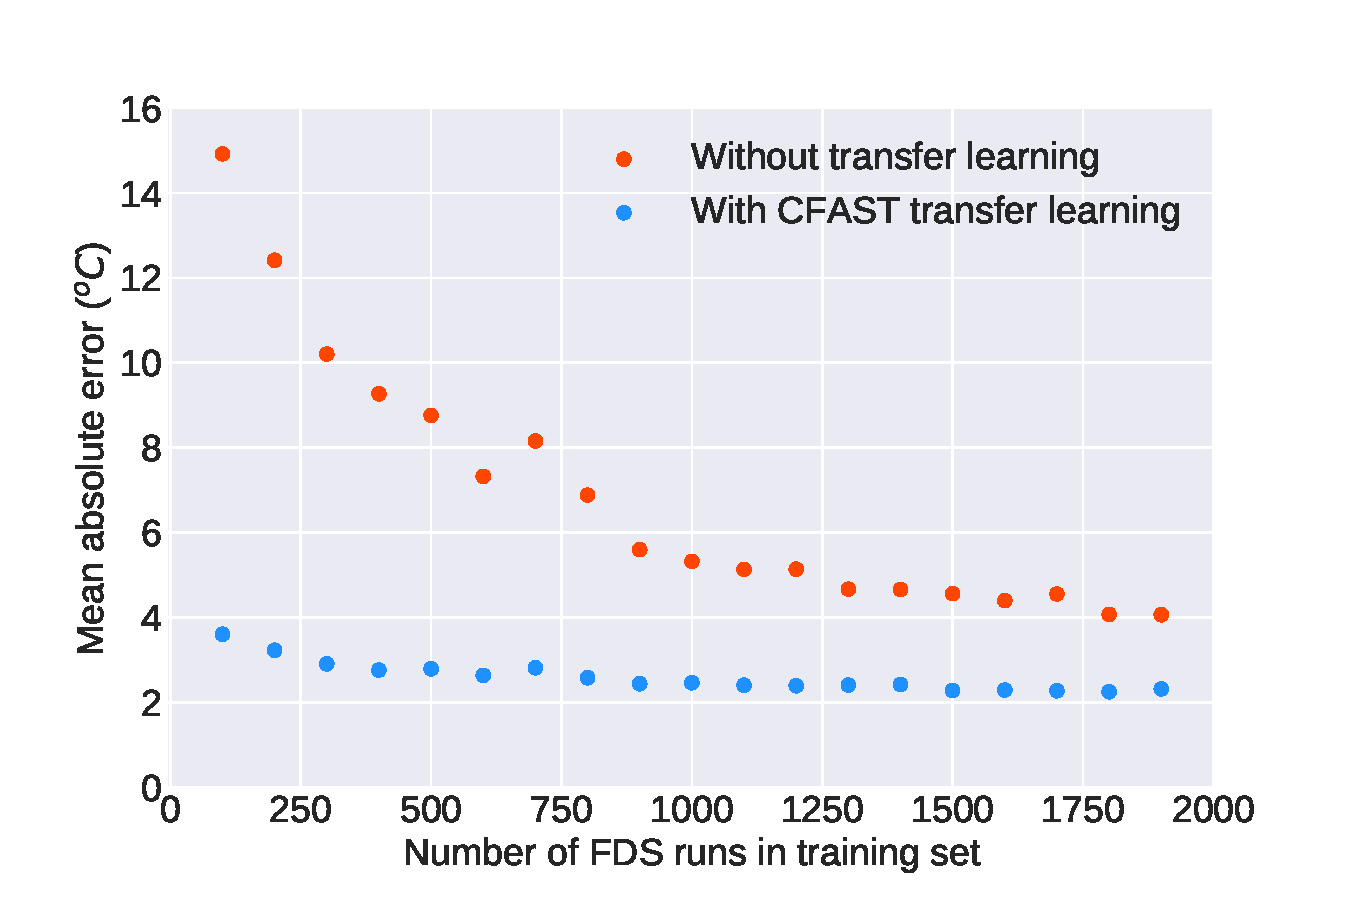
\includegraphics[width=.75\textwidth]{./figures/transfer_learning_effect.pdf}
\caption{A plot demonstrating the effect of transfer learning on the ability of an ANN to predict the response of a single thermocouple in FDS for a given HRR input. An ANN is first trained to predict the transient upper gas layer temperature given by CFAST, a simplified two zone fire model. Because of the simplified physics, a large training set (20,000 runs) is quickly obtained, allowing the ANN to accurately emulate CFAST. The weights and biases of this ANN are then used as the initial state of a second ANN that is trained to emulate the response of an individual thermocouple in FDS. The FDS emulator is scored based on its ability to predict the simulated thermocouple responses of 100 FDS cases that are excluded from the training sets. In each case, the ANNs train for 500 epochs.}
\label{fig:transfer_learning}
\end{figure}

These results indicate that an ANN trained using 1,900 FDS runs in isolation is unable to predict the FDS output as accurately as an ANN trained using 300 FDS runs with transfer learning. These results highlight the utility of simplified, computationally fast physical models to serve as stepping stones for ANNs to emulate more sophisticated models. Once one ANN is trained to predict the response of a thermocouple in FDS, its weights and biases are used as the initial state for the other 16 ANNs. Presumably, the task of predicting the simulated response of a thermocouple in FDS is more similar to predicting that of a thermocouple at a different location in FDS than predicting the upper layer temperature in CFAST.  

Based on the results in Figure \ref{fig:transfer_learning}, the emulators described hereafter are trained using the results from 1,000 FDS simulations and utilize transfer learning. In order to further characterize their accuracy, they predict the thermocouple responses of FDS simulations of the three curves shown in Figure $\ref{fig:training_ramps}$ These include two triangle fires, and a symmetric t-squared fire, all of which do not appear in the randomly generated training set. The predictions of the emulators are compared to the corresponding FDS simulations in Figure \ref{fig:forward_error}.

\begin{figure}[htbp]
  \centering
  \begin{subfigure}[t]{.45\textwidth}
      \centering
      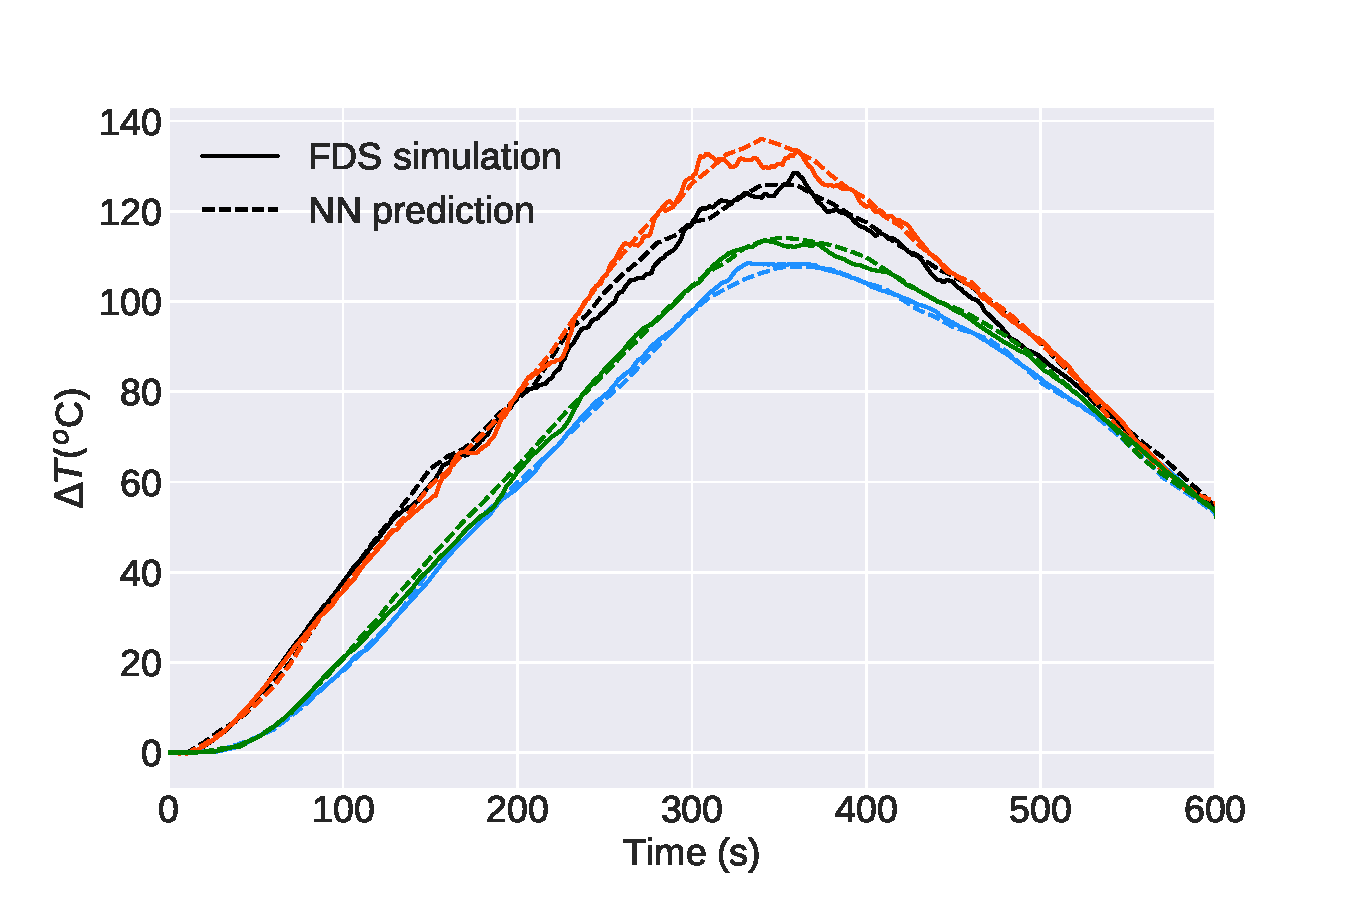
\includegraphics[width=\textwidth,keepaspectratio]{figures/forward_NN_examples.pdf}
      \caption{Example of emulator predictions compared to FDS simulations }
      \label{fig:forward_NN_examples}
  \end{subfigure}
  \begin{subfigure}[t]{.45\textwidth}
      \centering
      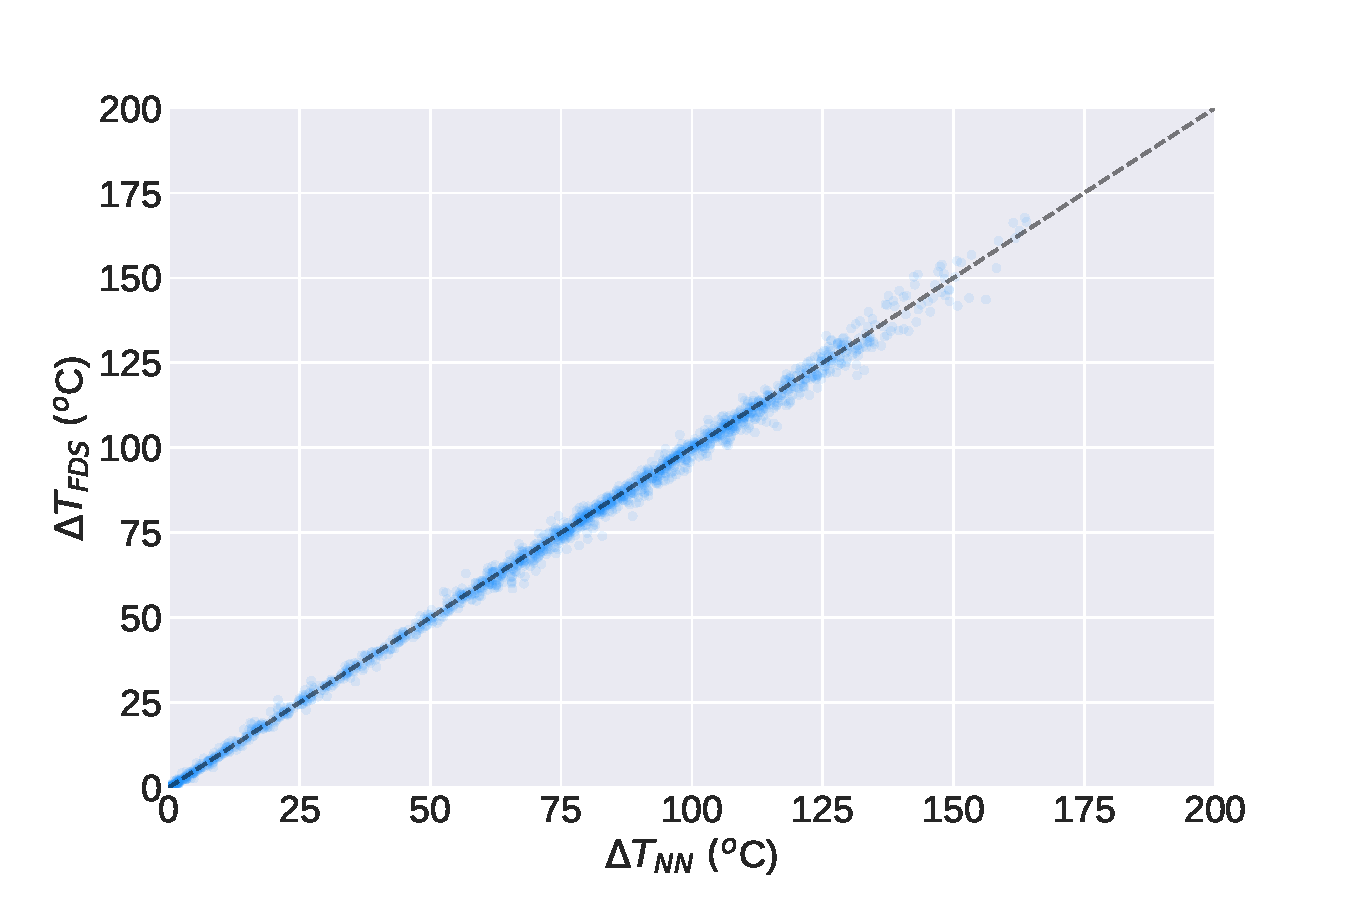
\includegraphics[width=\textwidth ,keepaspectratio]{figures/forward_error_scatter.pdf}
      \caption{Comparison of the FDS simulation results compared to the predictions from the emulators across all times, all three calibration set tests, and all 17 thermocouples }
      \label{fig:forward_error_scatter}
  \end{subfigure}
  \caption{A comparison of the predictions of the deep learning emulators compared to FDS simulations for the experimental fire ramps, which were not in the neural networks training set. \protect\ref{fig:forward_error_scatter} shows that the emulators successfully predict the FDS output with a mean absolute error of ~2$^o$ C across all sensors, all times, and all three experiments in Figure \protect\ref{fig:training_ramps}.} 
  \label{fig:forward_error}
\end{figure}

The emulators appear to reliably predict the output of FDS simulations that do not resemble the randomly drawn curves on which they trained. Also, the emulators are able to produce results for all 17 thermocouples at a rate of 120 times per second, compared to the about 25 minutes to run the FDS simulations. This is a speedup of over five orders of magnitude. 

Next the emulator predictions are compared to the measured thermocouple responses for the three burner experiments of Figure \ref{fig:training_ramps}. These results are shown in Figure \ref{fig:fds_vs_reality}.


\begin{figure}[htb] \centering
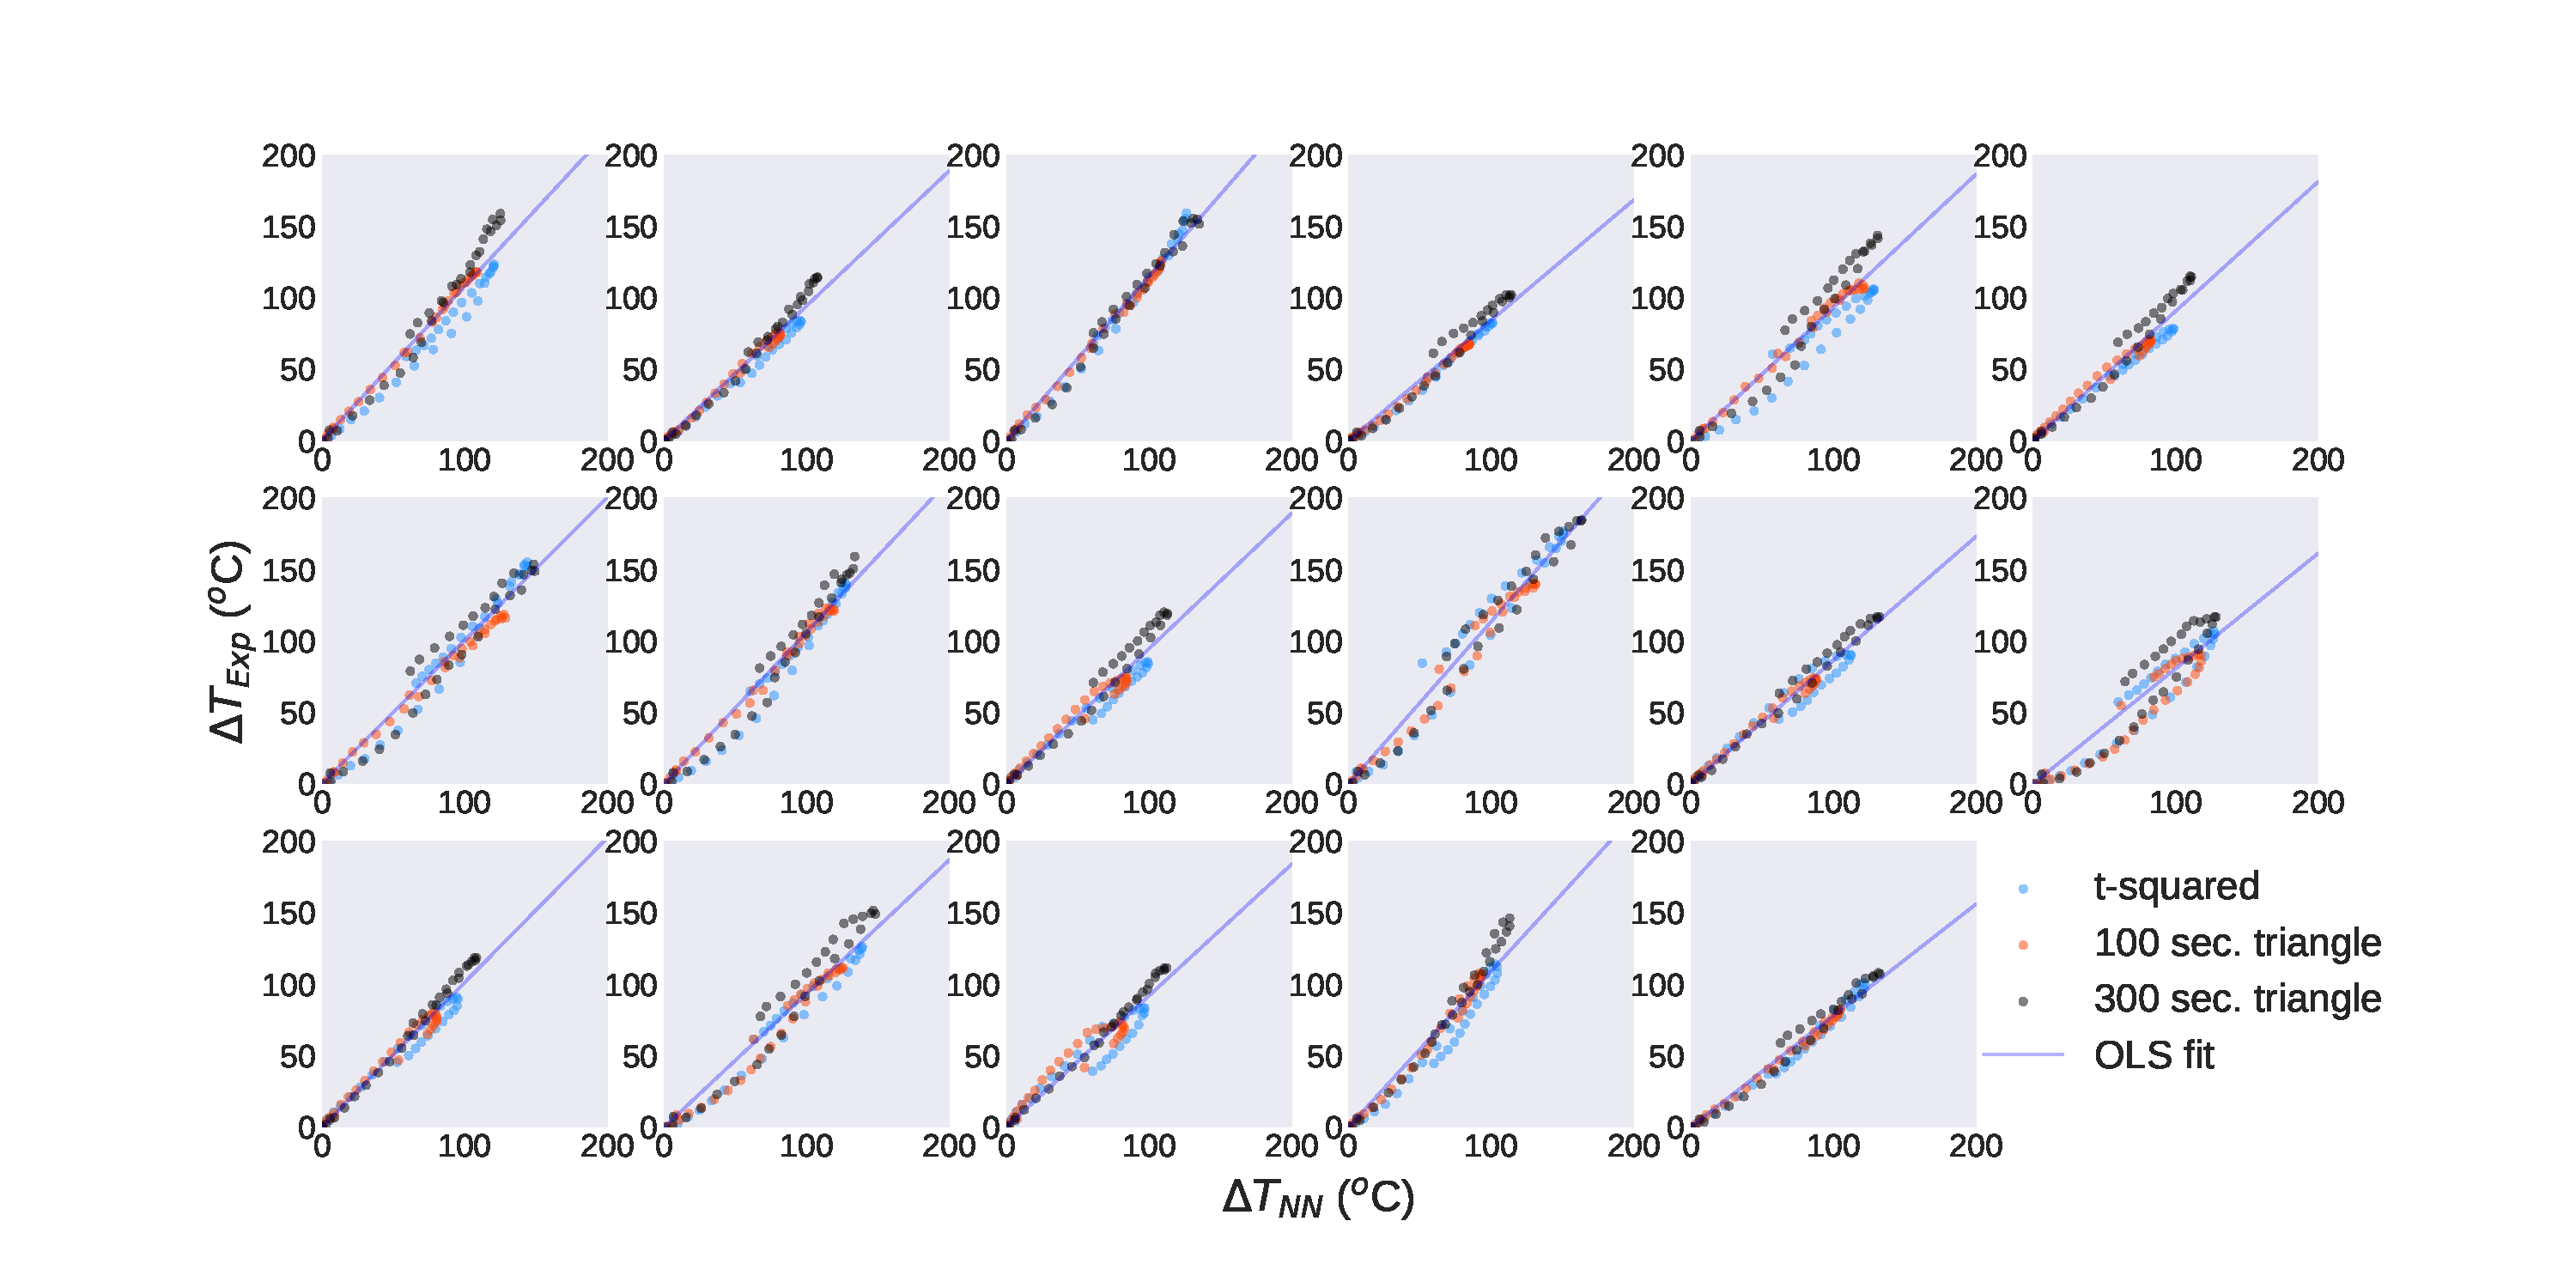
\includegraphics[width=1\textwidth]{figures/fds_vs_reality.pdf}
\caption{A comparison of the emulator predictions, $\Delta T_{NN}$, to the experimental measured temperatures $\Delta T_{Exp}$. Although the predictions are generally proportional to the experimentally measured temperatures, some predictions appear consistently biased. This is corrected by fitting an ordinary least squares (OLS) line to the experimental data as a function of the emulator predictions.}
\label{fig:fds_vs_reality}
\end{figure}

The FDS emulators generally produce accurate predictions of their respective thermocouple measurements for the three HRR experiments. Some predictions exhibit consistent bias, so an ordinary least squares (OLS) regression line is fit to correct this error. The bias is indicated by the fact that the plots in Figure \ref{fig:fds_vs_reality} are generally linear, but the slope of the relationship is not necessarily one. The OLS regression equation is described in equation \ref{eqn:bias_correct},  


\begin{equation}
  \label{eqn:bias_correct}
 \Delta \hat{T}_{exp, i} = \beta_i \Delta T _{NN, i}
\end{equation}

where $\Delta \hat{T}_{exp, i}$ is the predicted temperature measured by the $i$th thermocouple, $\beta_i$ is the slope of the OLS line, and $\Delta T _{NN, i}$ is the output of the FDS emulator for the $i$th thermocouple. An important consideration for determining $\beta_i$ is to ensure that each of the experiments have an equal impact in the OLS optimization. Without further data processing, the longer tests have a greater influence over the result because they have more measured and predicted points. To counteract this effect, 100 points are linearly interpolated for each experiment.  

After correcting for the biases, the ensemble model has the ability to make  fast and reasonably accurate predictions for all 17 measured temperature responses as a function of HRR. However, the model does not yet have the ability to estimate the heat release rate as a function of measured thermocouple temperaures. In order to add this component, a simple Bayesian parameter inversion is presented. The model outputs $\Delta \hat{T}_{exp, i}(\boldsymbol{t}^{NN})$ for all 17 thermocouples for a given $\dot{Q}(\boldsymbol{t}_{NN})$. When a new experiment takes place,  the experimental thermocouple temperature is measured, $\Delta T_{exp, i}(\boldsymbol{t}^{NN})$ for all 17 thermocouples. Note that interpolation may be necessary to make sure that the measurements coincide with $\boldsymbol{t}_{NN}$. A reasonable assumption is that the most likely HRR curve, $\dot{Q}(\boldsymbol{t}_{NN})$, is the one that produces model outputs that line up with the experimental measurements, i.e. $\Delta T_{exp, i}(\boldsymbol{t}^{NN}) \approx \Delta \hat{T}_{exp, i}(\boldsymbol{t}^{NN})$. Furthermore, the likelihood of a particular HRR curve can be quantified by calculating the corresponding amount of misfit between the model's output and the experimental data. This framework requires some description of the statistical distribution of misfitting. It may be tempting to assume that the modeling error for the $i$th thermocouple at the $j$th timestep,   $\epsilon_i(t^{NN}_j) = \Delta \hat{T}_{exp, i}(t^{NN}_j) - \Delta T_{exp, i}(t^{NN}_j)$ is independent and normally distributed. This is a flawed assumption because the error exhibit significant autocorrelation. This means that if the model is underpredicting or overpredicting at a specific timestep, the error will likely be similar in the next timestep. A better though still imperfect approach is to compute an aggregated measure of misfit for an entire prediction, such as the mean squared error, shown in equation \ref{eqn:MSE} for an individual thermocouple,

\begin{equation}
  \label{eqn:MSE}
 MSE_i = \frac{1}{N}\sum_{t \in \boldsymbol{t}_{NN} < t_{end}} \epsilon^2_i(t)
\end{equation}

\noindent where N is the number of elements in $\boldsymbol{t}_{NN}$ that are less than the duration of the test, $t_{end}$. Using the three experiments in the experimental calibration set, a distribution can be fitted to the observed MSE values. For three experiments with 17 predictions and measurements, there are 51 calculated MSE values. They are plotted in the histogram in Figure \ref{fig:misfit_pdf}. As expected, the distribution has a heavy tail to the right, but most of the values are relatively small. As a result, an exponential distribution is fitted to the data. This distribution is chosen for several reasons. First, it is monotonically decreasing, meaning that the likelihood of a particular HRR curve being ``correct" should increase as the error it produces in the model decreases. The exponential distribution also has a heavy tail to the right, and it is relatively easy to fit because it is uniquely characterized by a single parameter. The equation for the exponential distribution is shown in equation \ref{eqn:exponential_dist},

\begin{equation}
  \label{eqn:exponential_dist}
 p\bigg(MSE_i\Big(\dot{Q}(\boldsymbol{t}_{NN}) \Big)  \bigg) =  \lambda exp\bigg(-\lambda \ MSE_i\Big(\dot{Q}(\boldsymbol{t}_{NN}) \Big)\bigg)
\end{equation}

where $\lambda$ is the parameter that characterizes the distribution. This inverse of the parameter is the mean of the distribution, i.e. $E(MSE_i)=1/\lambda$. This allows for a fitted exponential distribution simply by computing the mean of the observed MSE values. The result of this fitting procedure is shown in \ref{fig:misfit_distribution}.


\begin{figure}[htbp]
  \centering
  \begin{subfigure}[t]{.45\textwidth}
      \centering
      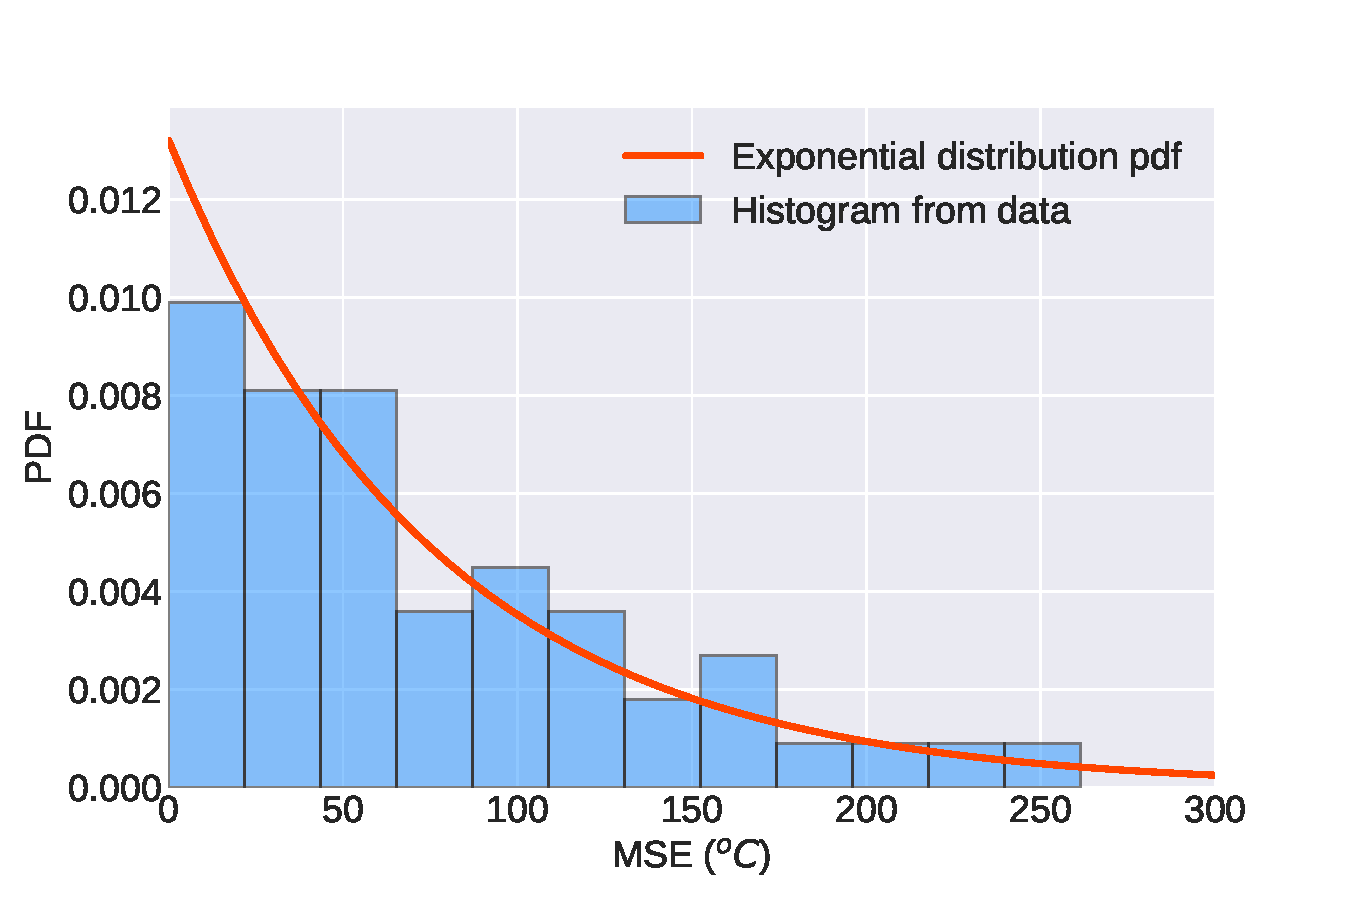
\includegraphics[width=\textwidth,keepaspectratio]{figures/misfit_pdf.pdf}
      \caption{A PDF of the fitted exponential distribution shown alongside a histogram of empirical data}
      \label{fig:misfit_pdf}
  \end{subfigure}
  \begin{subfigure}[t]{.45\textwidth}
      \centering
      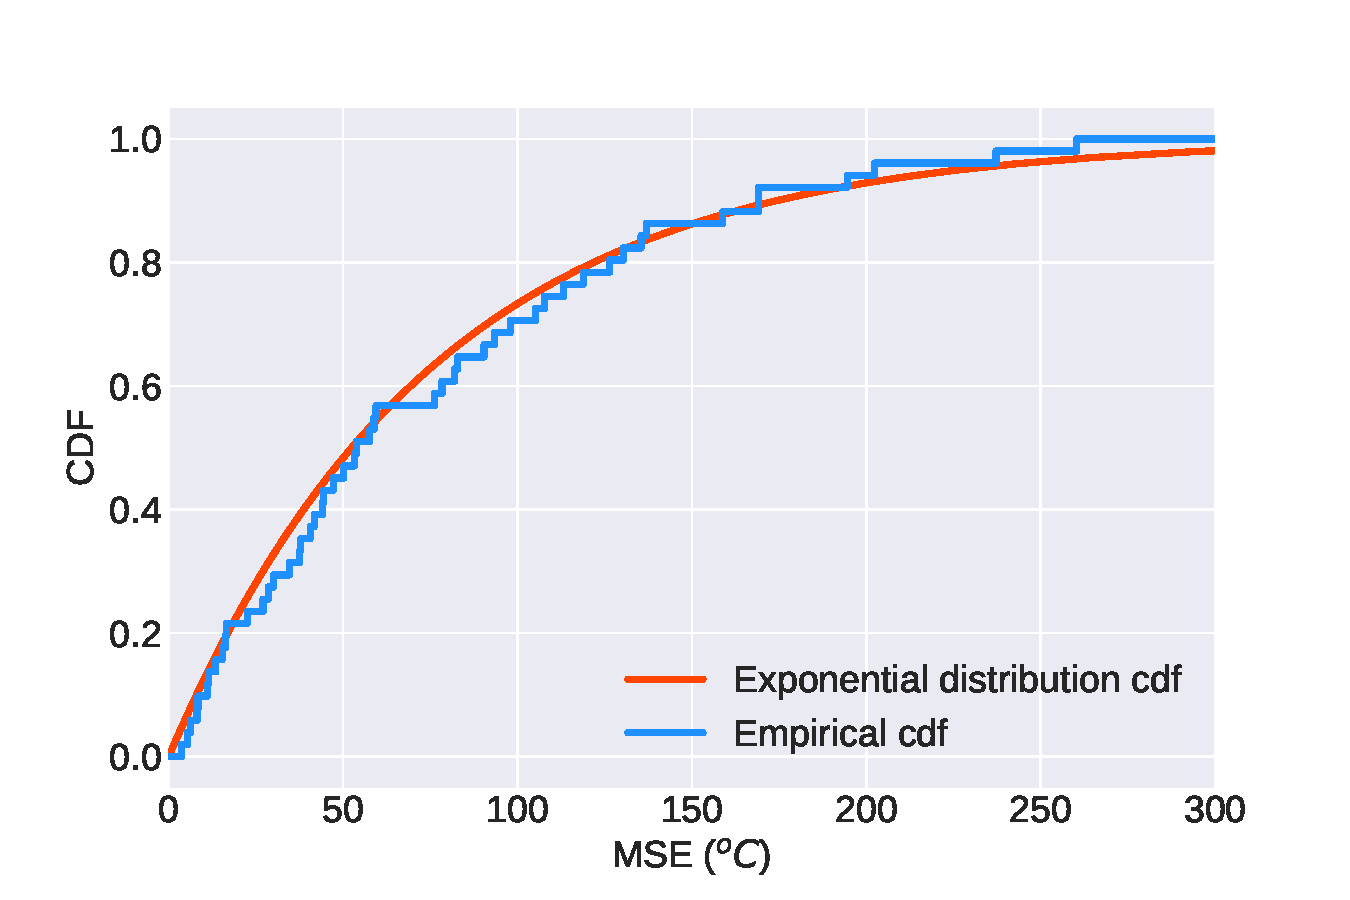
\includegraphics[width=\textwidth ,keepaspectratio]{figures/misfit_cdf.pdf}
      \caption{A CDF of the fitted exponential distribution shown alongside a CDF of empirical data}
      \label{fig:misfit_cdf}
  \end{subfigure}
  \caption{Comparison of the fitted exponential distribution to the actual distribution of MSE values} 
  \label{fig:misfit_distribution}
\end{figure}

Using the fitted exponential distribution, the likelihood of any HRR curve can be estimated based on the calculated MSE between the resulting $\Delta \hat{T}_{exp, i}$ and the actual measured temperatures, $\Delta {T}_{exp, i}$. If one specifies a prior for $\dot{Q}(t)$, then the exponential distribution likelihood allows for the calculation of a posterior distribution using Bayes law. The prior could be specified as a Gaussian process; however, a simpler approach is presented instead. The DFT measurements provide estimates of the radiative heat release rate, $\dot{Q}_R(t)$. This quantity is related to the total heat release rate by $\dot{Q} = \frac{\dot{Q}_R}{\chi_R}$. This allows a prior distribution to be placed on $\chi_R$, and the posterior distribution gives an estimate of $\dot{Q}$. Assuming that the DFT model provides the radiative heat release rate, the MSE can be written as a function of $\chi_R$ as follows:

\begin{equation}
  \label{eqn:MSE_chi_R}
MSE_i\Big(\dot{Q}(\boldsymbol{t}_{NN}) \Big) = MSE_i\Big( \frac{\dot{Q}_R(\boldsymbol{t}_{NN})}{\chi_R}\Big) \approx MSE_i\Big( \frac{\dot{Q}^{\text{GP}}_R(\boldsymbol{t}_{NN})}{\chi_R}\Big) = MSE_i\Big( \chi_R\Big)
\end{equation}

\noindent Note that in the previous section, the output of the DFT model is $\dot{Q}_{R}^{\text{GP}}(\boldsymbol{t^{\text{DFT}}})$. Obtaining $\dot{Q}^{\text{GP}}_R(\boldsymbol{t}_{NN})$ is trivial because all of the times in $\boldsymbol{t}_{NN}$ are in $\boldsymbol{t}^{\text{DFT}}$, except times that are after $t_{end}$. For these times, $\dot{Q}^{\text{GP}}_R(\boldsymbol{t}_{NN})$ is set to zero. 

A posterior distribution for $\chi_R$ can be obtained by placing a prior on $\chi_R$ and using Bayes' law with the fitted exponential distribution as the likelihood, i.e. $p\big(\chi_R | \Delta T_{exp,i}(\boldsymbol{t}_{NN}) \big) = p\Big(MSE_i\big(\chi_R\big) \Big)$. Bayes law is then 

\begin{equation}
  \label{eqn:forward_bayes}
p\big(\chi_R | \boldsymbol{\Delta T}_{exp} \big) \propto p(\chi_R) \prod_{i=1}^{17} p\Big(MSE_i\big(\chi_R\big) \Big)
\end{equation}


\noindent where $p(\chi_R)$ is the prior distribution for $\chi_R$. A uniform prior between 0.20 and 0.45 is used for $\chi_R$, i.e. $\chi_R \sim Uniform(0.20, 0.45)$. Equation \ref{eqn:forward_bayes} updates the distribution for $\chi_R$ in light of the experimentally measured temperatures. Also note that equation \ref{eqn:forward_bayes} assumes the MSE values are independent across the thermocouple predictions. This assumption is not perfect, but it removes the need for independently distributed residuals ($\epsilon _i$) in time. Finally, the marginal likelihood, $p(\boldsymbol{\Delta T}_{exp})$, is omitted because it does not need to be calculated directly. Instead, the proportional form of Bayes' law is all that is necessary because the result is scaled to ensure a valid probability distribution that integrates to one. 

The results of the Bayesian inference procedure are shown in Figure \ref{fig:bayes_result}. 


\begin{figure}[htbp]
  \centering
  \begin{subfigure}[t]{.45\textwidth}
      \centering
      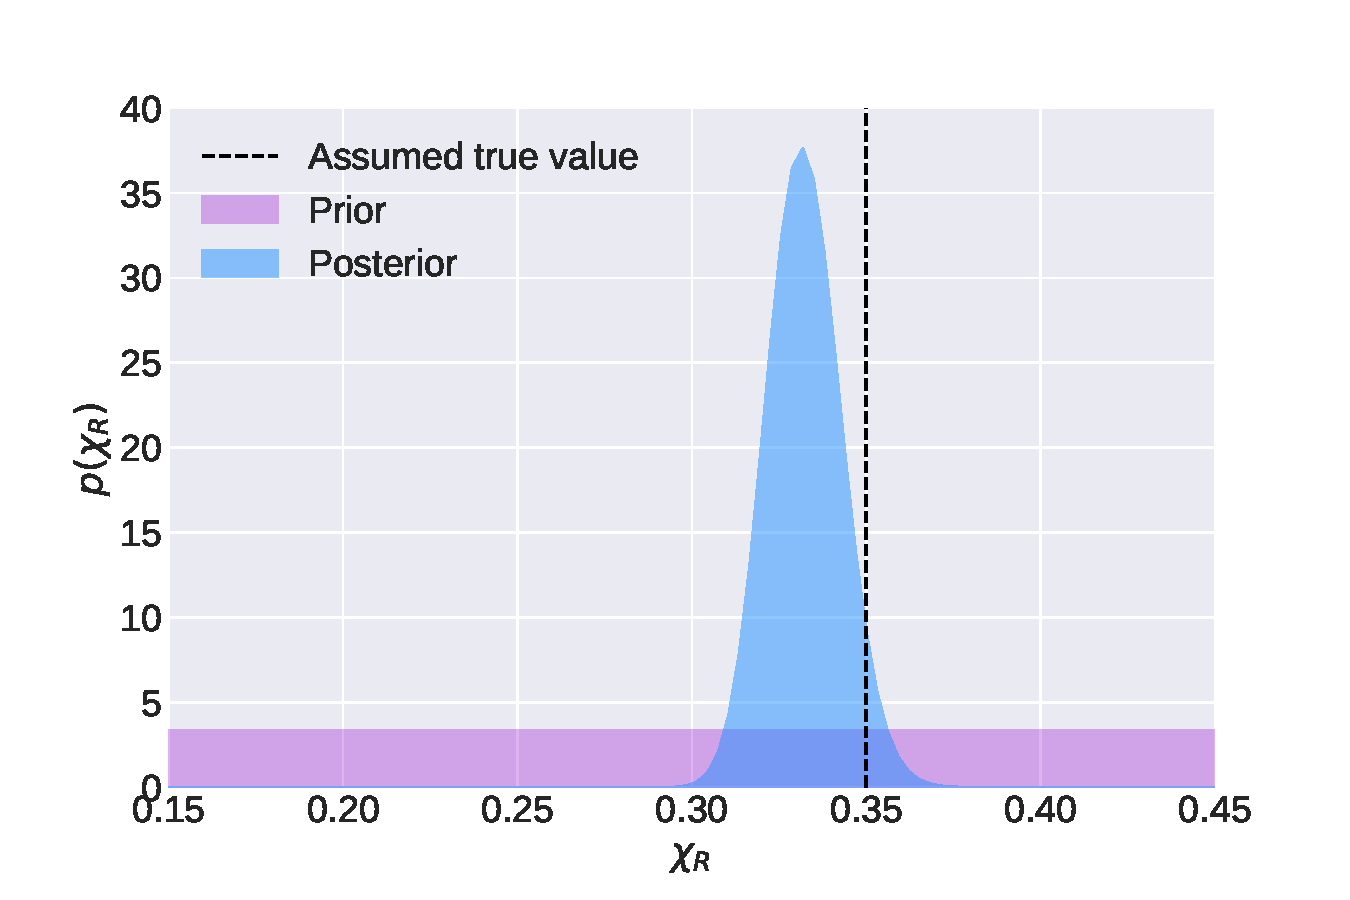
\includegraphics[width=\textwidth,keepaspectratio]{figures/bayes_distributions.pdf}
      \caption{Distributions for $\chi_R$}
      \label{fig:bayes_distributions}
  \end{subfigure}
  \begin{subfigure}[t]{.45\textwidth}
      \centering
      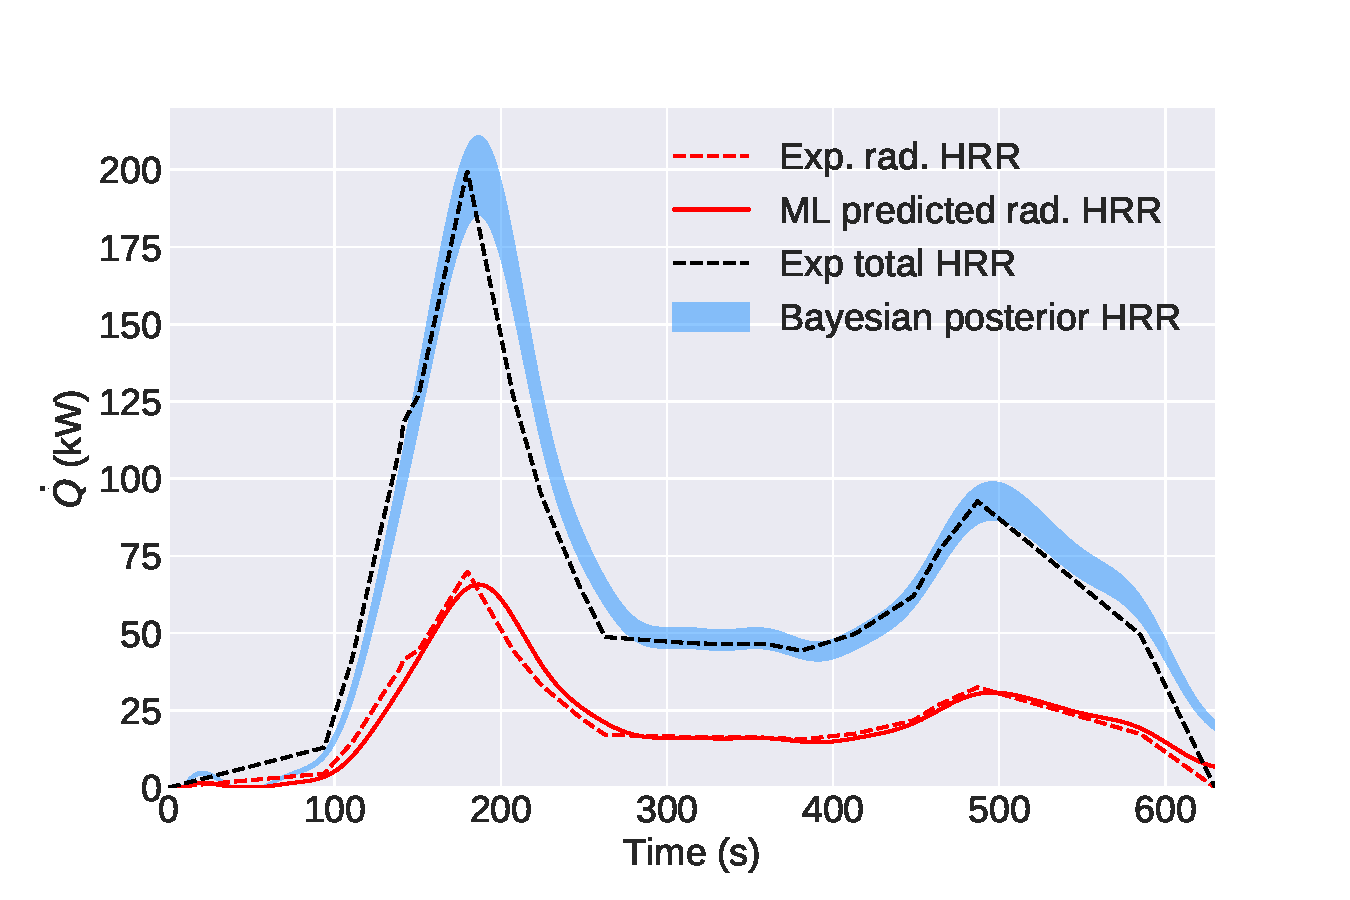
\includegraphics[width=\textwidth ,keepaspectratio]{figures/bayes_burner_result.pdf}
      \caption{Corresponding HRR prediction using 95\% confidence interval}
      \label{fig:burner_result}
  \end{subfigure}
  \caption{Result of the Bayesian inference procedure for the ``test" curve. \protect\ref{fig:bayes_distributions} shows the prior and posterior distributions for $\chi_R$. Note how the assumed value of $\chi_R$ for propane, 0.35, is inside the posterior distribution. The posterior distribution for $\chi_R$ then gives estimates of the total HRR by the relation $\dot{Q}(t) = \frac{\dot{Q}_R(t)}{\chi_R}$. The radiative HRR and the corresponding estimate, $\dot{Q}^{\text{GP}}_R(\boldsymbol{t}_{NN})$ are also shown. }
  \label{fig:bayes_result}
\end{figure}





\clearpage
\subsubsection{Backward FDS emulators}

Another approach for estimating $\dot{Q}(t)$ which uses only the thermocouple measurements is presented. Unlike the approach described in the previous secition which uses an array of ANNs that map the HRR to an array of simulated thermocouple responses, the approach presented here maps the thermocouple response to the FDS input HRR for each of the 17 thermocouples. The transfer learning procedure is similar to that described in the previous section. However, the first ANN is learnes to predict the transient HRR input to CFAST given the outputted upper gas layer temperature. The parameters of this ANN is then used as the initial state of the first ANN that predicts the HRR input in FDS given a simulated thermocouple response. The parameters of the first ``backward" FDS emulator are then used as the initial state of the remaining 16 FDS backward emulators. 


The accuracy of these emulators is shown in Figure \ref{fig:backward_examples}.

\begin{figure}[htbp]
  \centering
  \begin{subfigure}[t]{.45\textwidth}
      \centering
      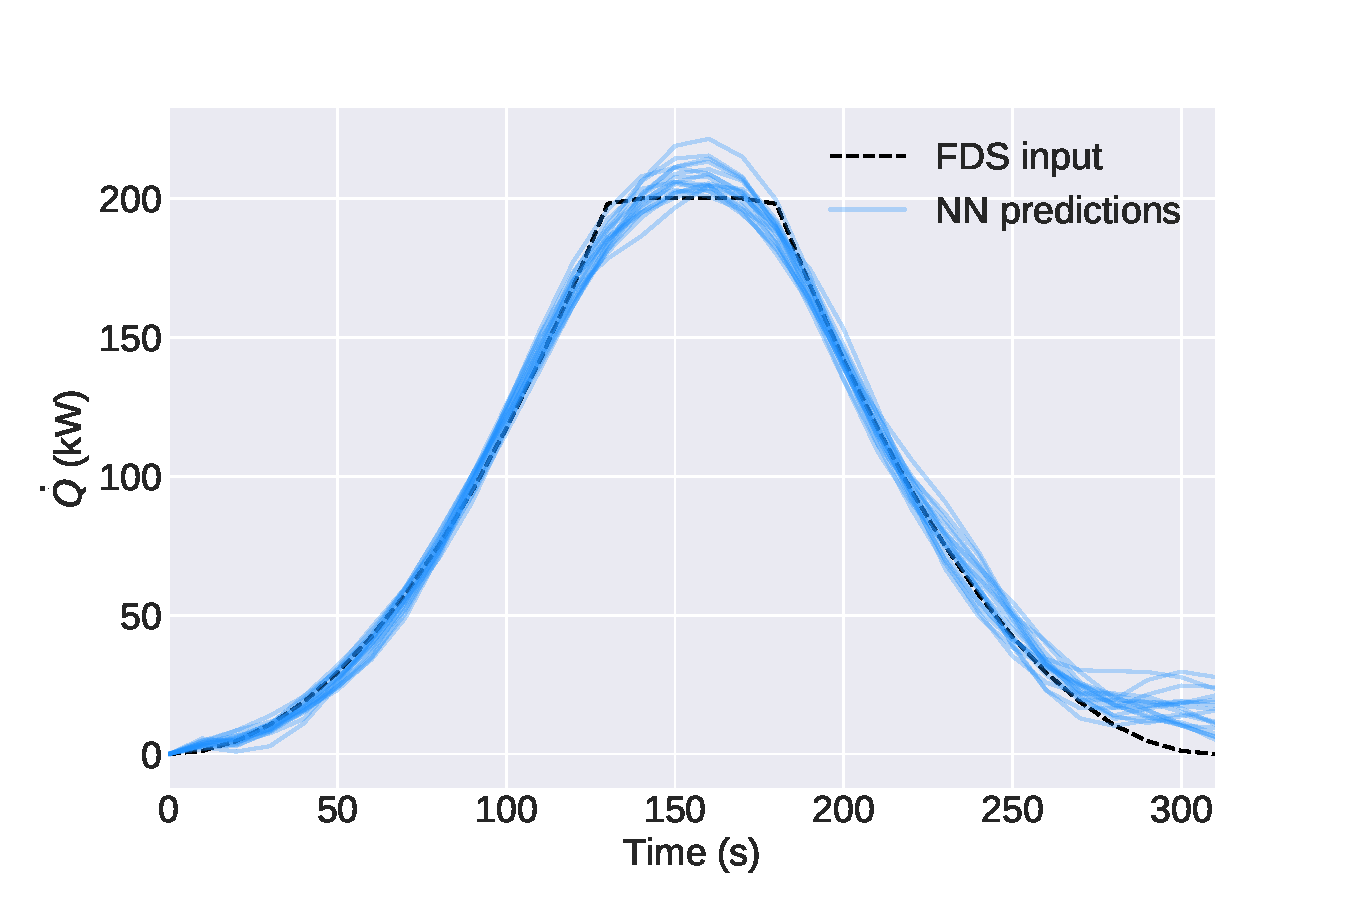
\includegraphics[width=\textwidth,keepaspectratio]{figures/backward_NN_examples.pdf}
      \caption{}
      \label{fig:backward_NN_examples}
  \end{subfigure}
  \begin{subfigure}[t]{.45\textwidth}
      \centering
      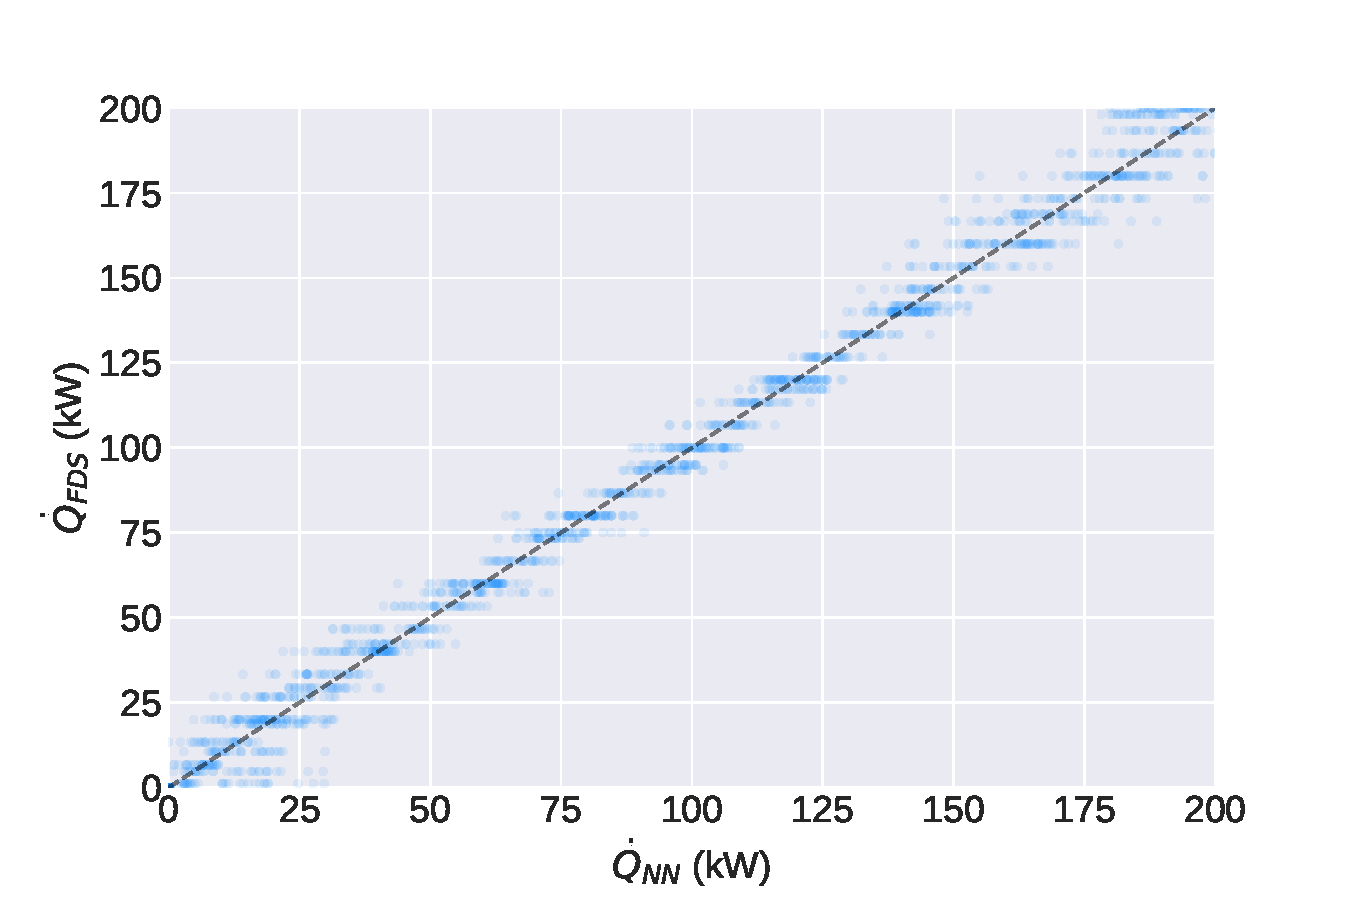
\includegraphics[width=\textwidth ,keepaspectratio]{figures/backward_error_scatter.pdf}
      \caption{}
      \label{fig:backward_error_scatter}
  \end{subfigure}
  \caption{Predictions of the backward FDS emulators compared to the actual HRR inputs. In \protect\ref{fig:backward_NN_examples}, the dashed black line was the input to an FDS simulation, which produced simulated thermocouple responses for 17 different locations. Each of the 17 outputs are then fed into its corresponding backward FDS emulator, which attempts to predict the HRR input. The 17 blue lines show the predicted HRR input from each of the 17 backward emulators. \protect\ref{fig:backward_error_scatter} shows the actual HRR input compared to the preditions from the backward emulator for FDS simulations of the three ramps of Figure \protect\ref{fig:training_ramps}.} 
  \label{fig:backward_examples}
\end{figure}

The backward emulators can then make predictions of the HRR based on experimental data. For a measured thermocouple response, the each emulator predicts the HRR input that would produce the corresponding simulation output in FDS. From each thermocouple response,  $\Delta T_{exp_i} (\boldsymbol{t}_{NN})$ (a vector), the corresponding backward emulator produces an estimate of the heat release rate, $\Dot{Q}^{\text{NN}}_i (\boldsymbol{t}_{NN})$ (also a vector). Using all 17 backward emulators, a 91x17 feature matrix is constructed for a single experiment, $\Dot{Q}^{\text{NN}} (\boldsymbol{t}_{NN})$. It is now reasonable to use a linear model for these features because the physical model (FDS) has accounted for the the previously described hysteresis issue. The linear model is described below in equation \ref{eqn:backward_ridge}, 

\begin{equation}
  \label{eqn:backward_ridge}
    \Dot{Q}^{\text{est}}(\boldsymbol{t}_{NN}) = \Dot{Q}^{\text{NN}} (\boldsymbol{t}_{NN})\boldsymbol{\beta}
\end{equation}

\noindent where $\Dot{Q}^{\text{est}}(\boldsymbol{t}_{NN})$ is the final estimate of the HRR curve given the feature matrix and $\boldsymbol{\beta}$ is a vector of weights or regression slopes. Another way to think of this procedure is that the estimated HRR is a weighted sum of the estimates from the backward emulators. The weights are then calculated using the experiments in the calibration set. This approach makes it so that the model places more weights in sensors that produce reliable estimates. In this case, regularization is still advantageous because the features are correlated (multicollinearity) and overfitting is a concern with with high dimensional regressions. However, the feature selection was already performed; the thermocouples above 1.5 m off the ground were chosen because they are most sensitive to the quantity of interest and their simulation results are not significantly affected by the use of a coarse mesh. As a result, a ridge regression is employed over a lasso regression. This produces the benefits of regularization without removing features. Using the ridge regression framework, the weights are calculated according to equation \ref{eqn:ridge_weights}.


 \begin{equation}
  \label{eqn:ridge_weights}
  \hat{\boldsymbol{\beta}}_{ridge} = \argmin_{\boldsymbol{\beta}}\Bigg\{ \underbrace{\big[\boldsymbol{\dot{Q}} - \boldsymbol{\Dot{Q}}^{\text{NN}} \boldsymbol{\beta}  \big]^T \big[\boldsymbol{\dot{Q}} - \boldsymbol{\Dot{Q}}^{\text{NN}}\boldsymbol{\beta}\big]}_{\text{I}} + \underbrace{\lambda||\boldsymbol{\beta}||_2}_{II}   \Bigg\}
\end{equation}

This equation is very similar to equation \ref{eqn:lasso}, which describes the lasso regression. The key difference is the use of the L2 norm as opposed to the L1 norm in term II. This is analogous to the use of a a circle as opposed to a diamond in Figure \ref{fig:lasso_graphic}. The vector, $\boldsymbol{\Dot{Q}}^{\text{NN}}$, and the matrix, $\boldsymbol{\Dot{Q}}^{\text{NN}}$, are slightly different than previously described. When making predictions for a new experiment, an intermediate step is computing the feature matrix, $\Dot{Q}^{\text{NN}} (\boldsymbol{t}_{NN})$, which contains emulator results at the vector of times, $\boldsymbol{t}_{NN}$. When calculating $\hat{\boldsymbol{\beta}}_{ridge}$, there are actually three separate experiments that comprise the feature matrix. One may think that the feature matrix used for this step would then be 293x17 because there are three calibration tests, each with measurements at the 91 points in $\boldsymbol{t}_{NN}$. However, the observed heat release rate at many of these points would be zero because $\boldsymbol{t}_{NN}$ includes times up to 900 seconds, and none of the tests are this long. For times greater than the duration of the experiment, $t_{end}$, the observed HRR values are zero, and the emulator outputs are also usually zero. As a result, these points do not significantly inform the calculation of $\beta$ and thus, longer experiments are weighted more heavily than shorter experiments. To circumvent this issue, 100 points are interpolated between 0 and $t_{end}$ for each experiment. Therefore, $\boldsymbol{\dot{Q}}$ is a vector of length 300, containing the interpolated experimental HRR at a 100 points for each experiment, and $\boldsymbol{\Dot{Q}}^{\text{NN}}$ is the corresponding 300x17 matrix of interpolated emulator outputs. Again, the hyperparameter $\lambda$ is chosen using 5-fold cross validation as before. The results of this inversion approach are shown in Figure \ref{fig:backward_ridge_aggregation}.

\begin{figure}[htb] \centering
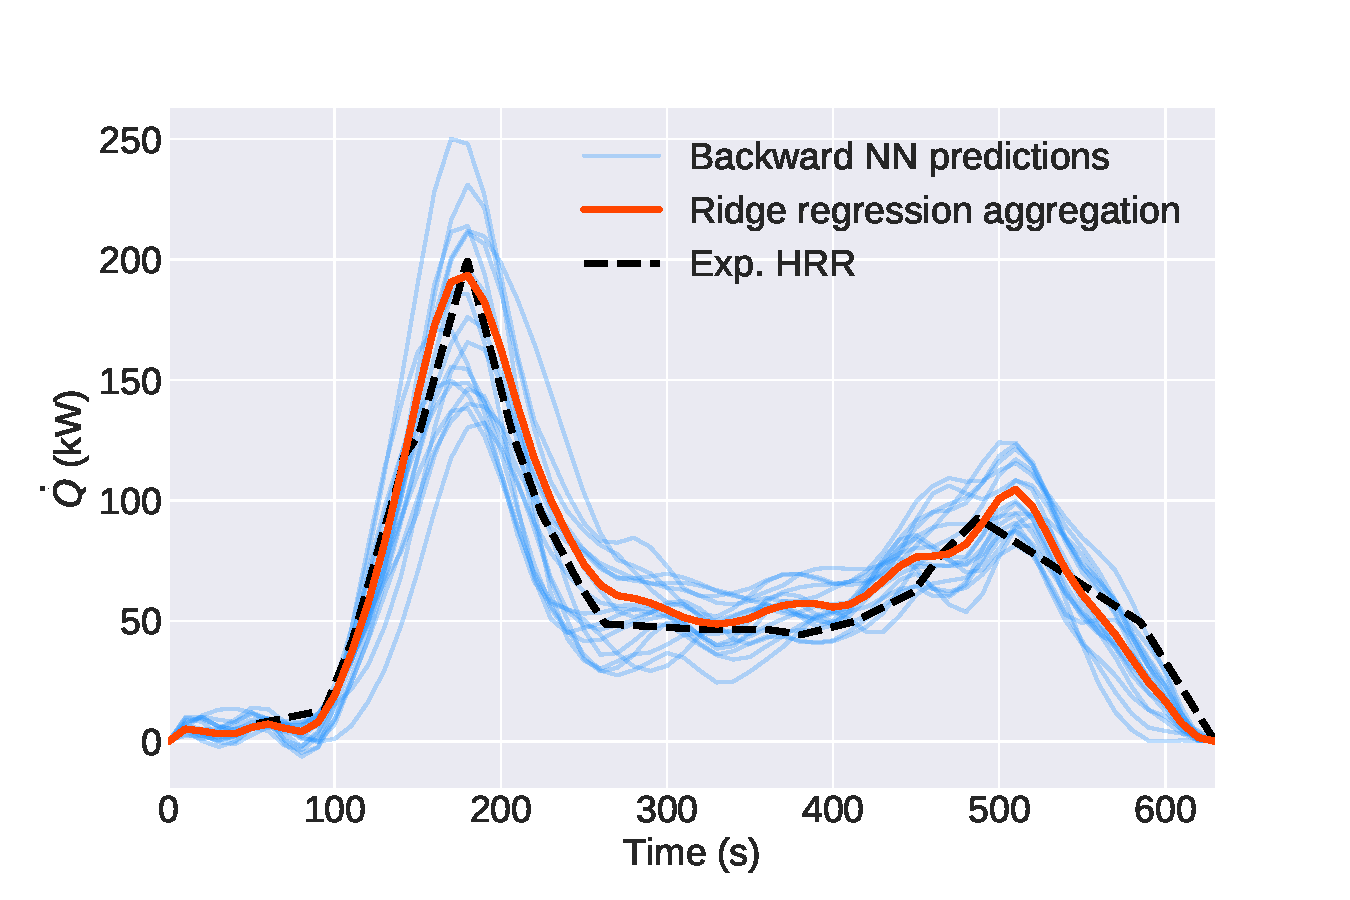
\includegraphics[width=.75\textwidth]{figures/backward_ridge_aggregation.pdf}
\caption{Visual summary of the ``backward" emulator HRR inversion framework. For each thermocouple, the response is inputted to an ANN that predicts the HRR input to FDS that would result in a corresponding simulation output. This is done for each of the 17 thermocouples resulting in the 17 blue lines. Using the data from the calibration experiments, a ridge regression produces a weighted sum of the 17 HRR estimates (the red line). The weights are determined using equation \protect\ref{eqn:ridge_weights}.}
\label{fig:backward_ridge_aggregation}
\end{figure}


In order to gain a better idea of the models' ability to estimate the HRR curve for new burner fires, the methods are conducted a total of four times, using each of the four burner experiments as the test curve while the other three are used as calibration curves. These results are shown in Figure \ref{fig:final_burner_results}.

\begin{figure}[htbp]
  \centering
  \begin{subfigure}[t]{.45\textwidth}
      \centering
      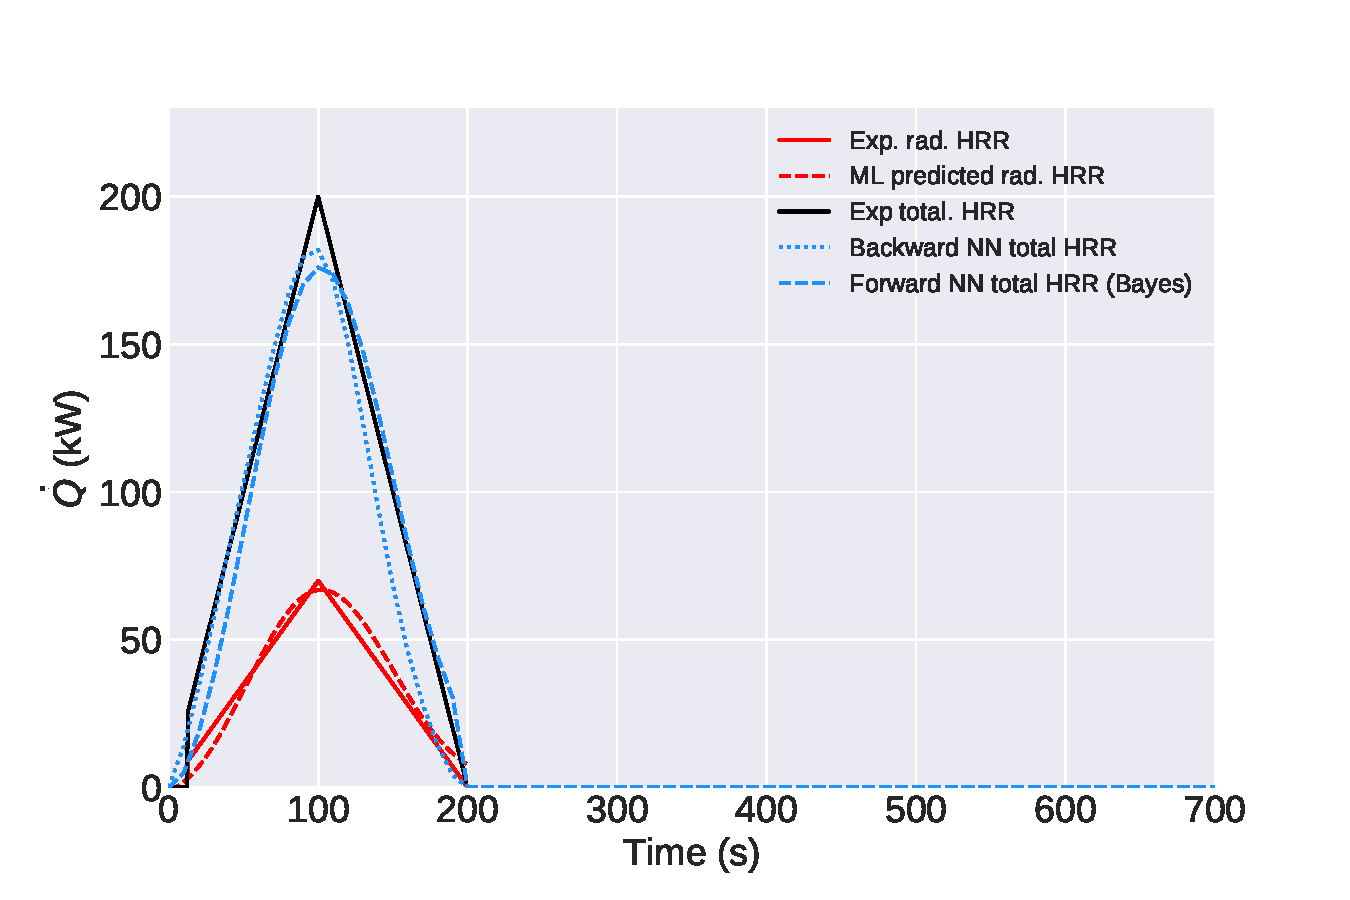
\includegraphics[width=\textwidth,keepaspectratio]{figures/100s_triangle_final.pdf}
      \caption{100 sec. triangle \\ Forward: MAE = 8.9 kW (9.0 \%) \\ Backward: MAE = 13.1 kW (13.2 \%)}
      \label{fig:final_result_100s_triangle}
  \end{subfigure}
  \begin{subfigure}[t]{.45\textwidth}
      \centering
      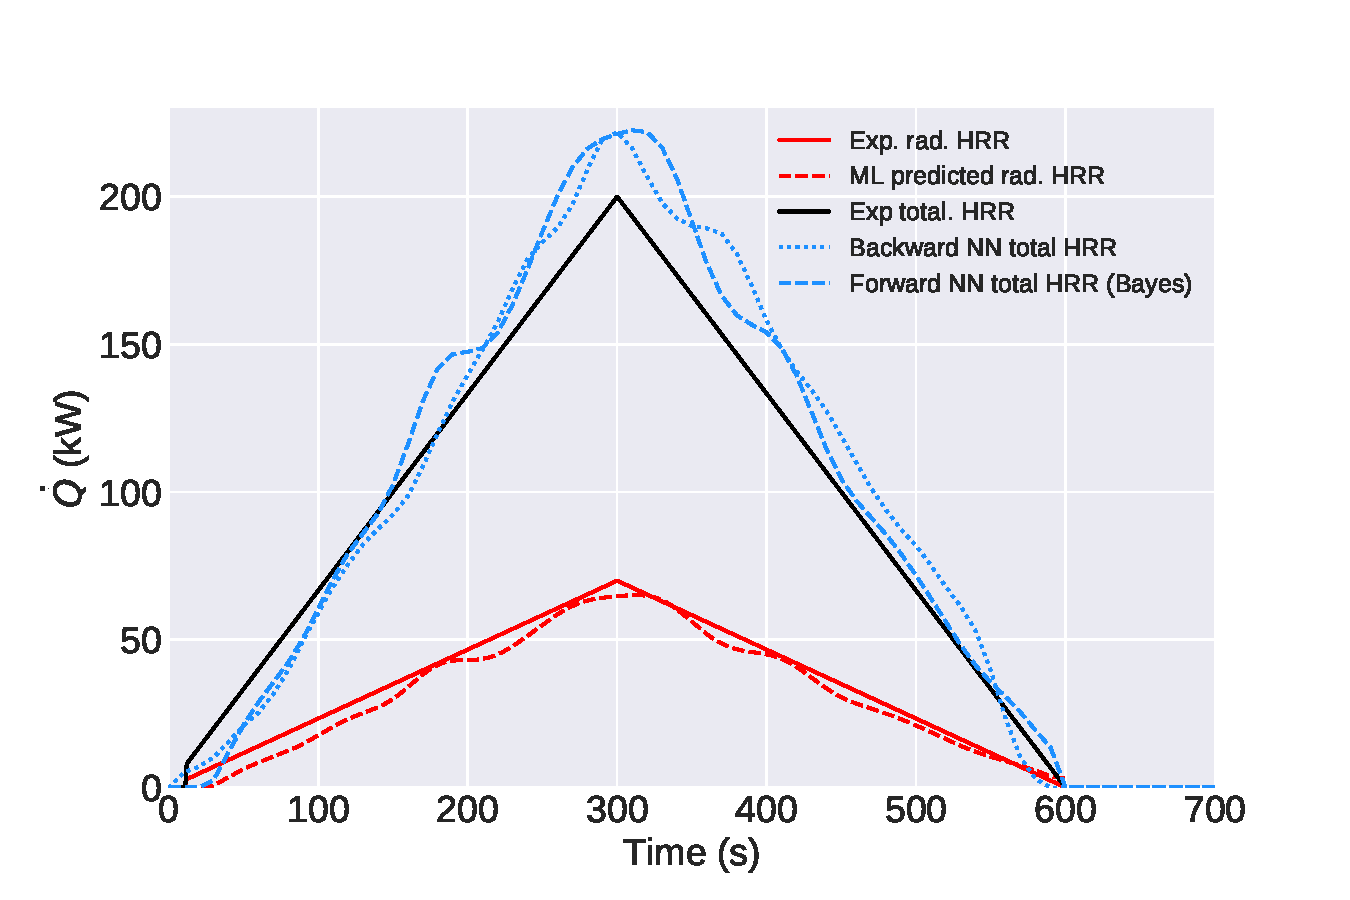
\includegraphics[width=\textwidth ,keepaspectratio]{figures/300s_triangle_final.pdf}
      \caption{300 sec. triangle \\ Forward: MAE = 12.7 kW (12.7 \%) \\ Backward: MAE = 14.3 kW (14.3 \%)}
      \label{fig:final_result_300s_triangle}
  \end{subfigure}
   \begin{subfigure}[t]{.45\textwidth}
      \centering
      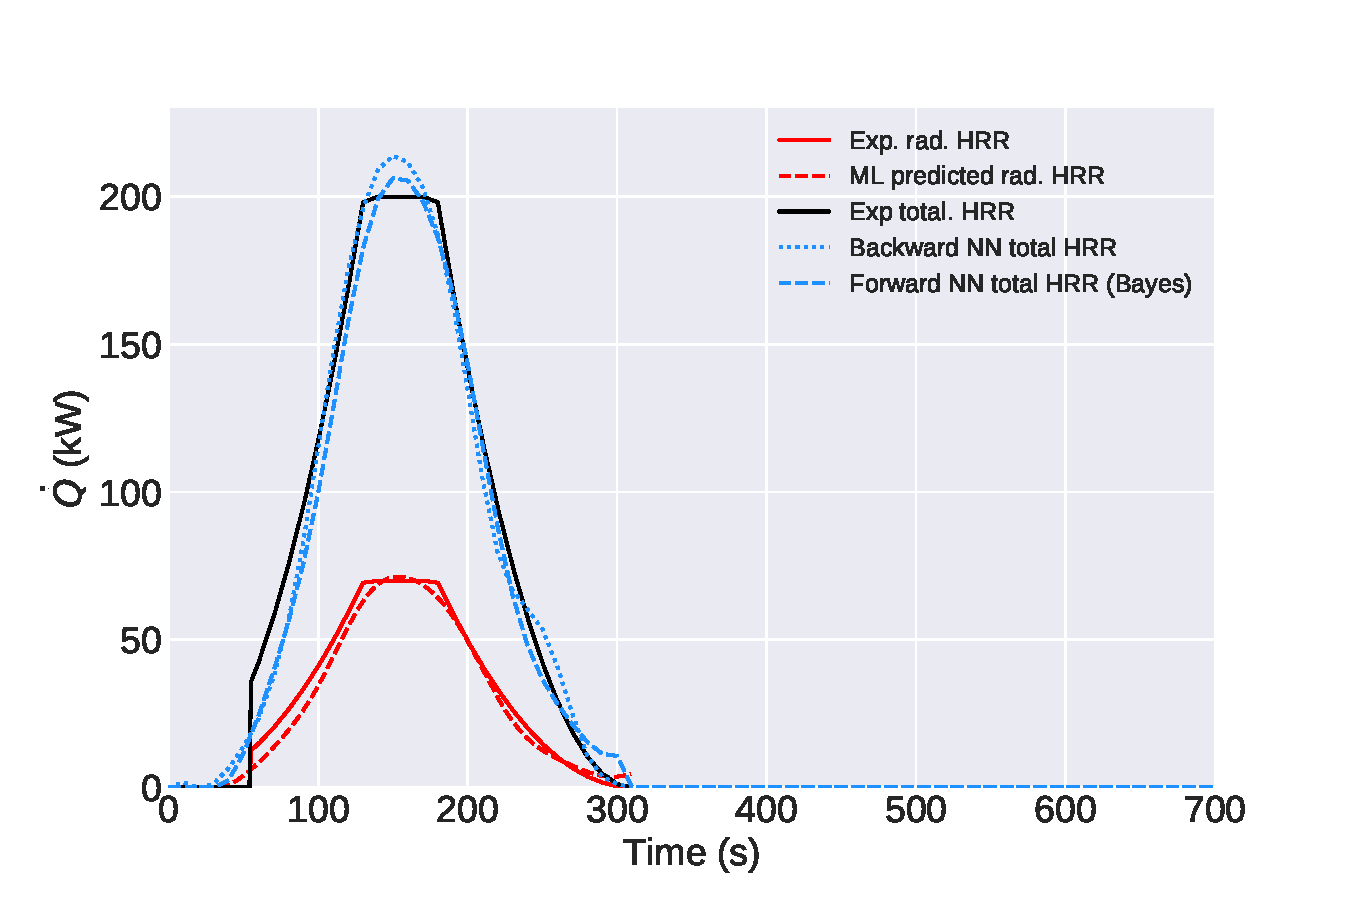
\includegraphics[width=\textwidth ,keepaspectratio]{figures/t_squared_final.pdf}
      \caption{t-squared \\ Forward: MAE = 7.4 kW (8.7 \%) \\ Backward: MAE = 7.4 kW (8.7 \%)}
      \label{fig:final_result_t_squared}
  \end{subfigure}
    \begin{subfigure}[t]{.45\textwidth}
      \centering
      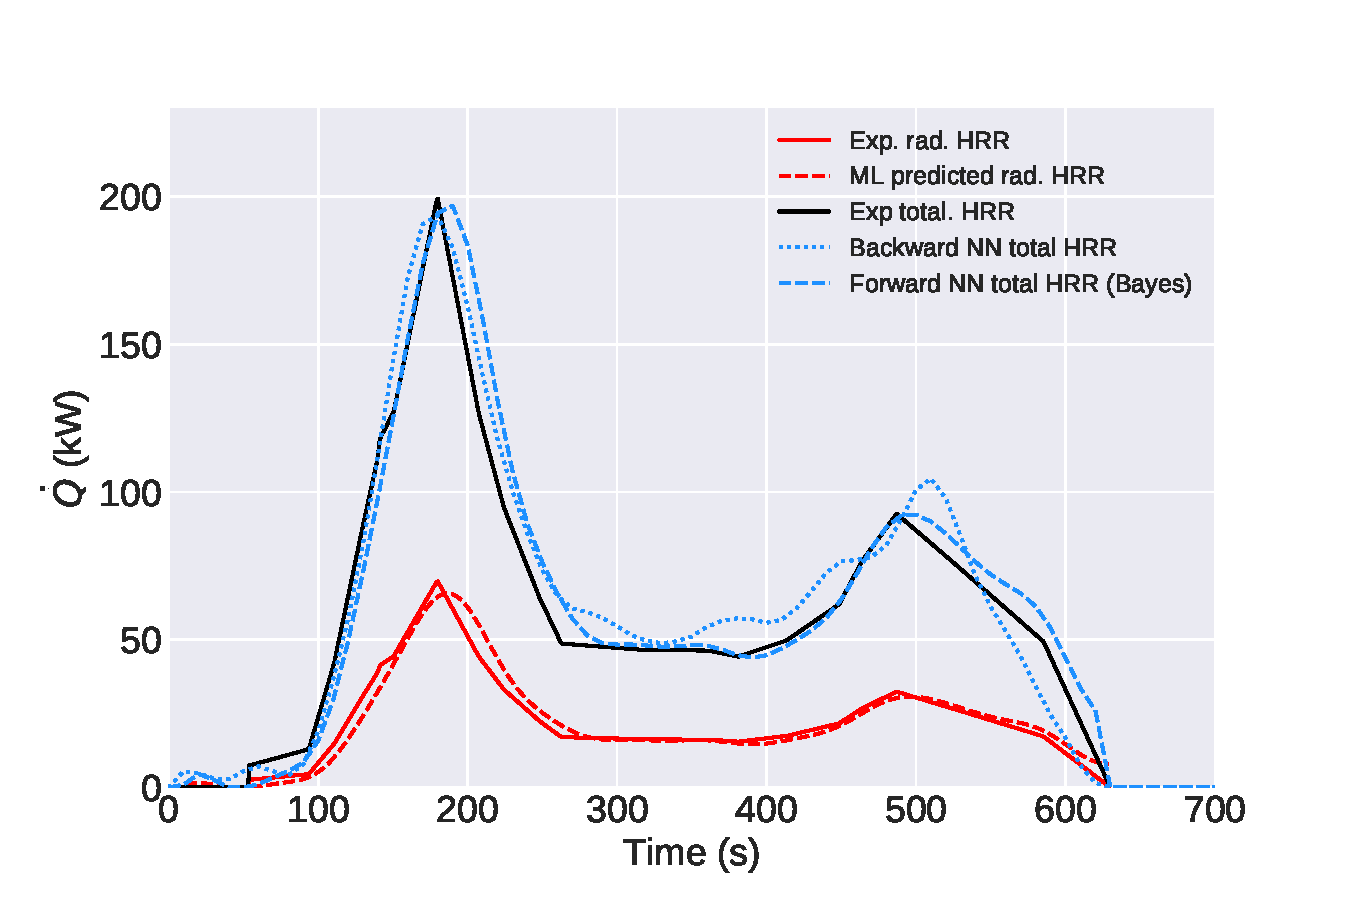
\includegraphics[width=\textwidth ,keepaspectratio]{figures/weird_curve_final.pdf}
      \caption{Arbitrary curve \\ Forward: MAE = 7.1 kW (11.6 \%) \\ Backward: MAE = 9.0 kW (14.7 \%)}
      \label{fig:final_result_weird_curve}
  \end{subfigure}
  \caption{HRR inversion results for all four burner experiments. For each case, the other three experiments are used for calibration while the shown experiment is excluded.} 
  \label{fig:final_burner_results}
\end{figure}

The models were also exercised on n-Hexane and methanol pool fires. The image regression method is excluded due to the difficulty of identifying the flame region of the nearly transparent methanol flames. The results from two n-Hexane experiments are shown in Figure \ref{fig:nhex_fires}.

\begin{figure}[htbp]
  \centering
  \begin{subfigure}[t]{.45\textwidth}
      \centering
      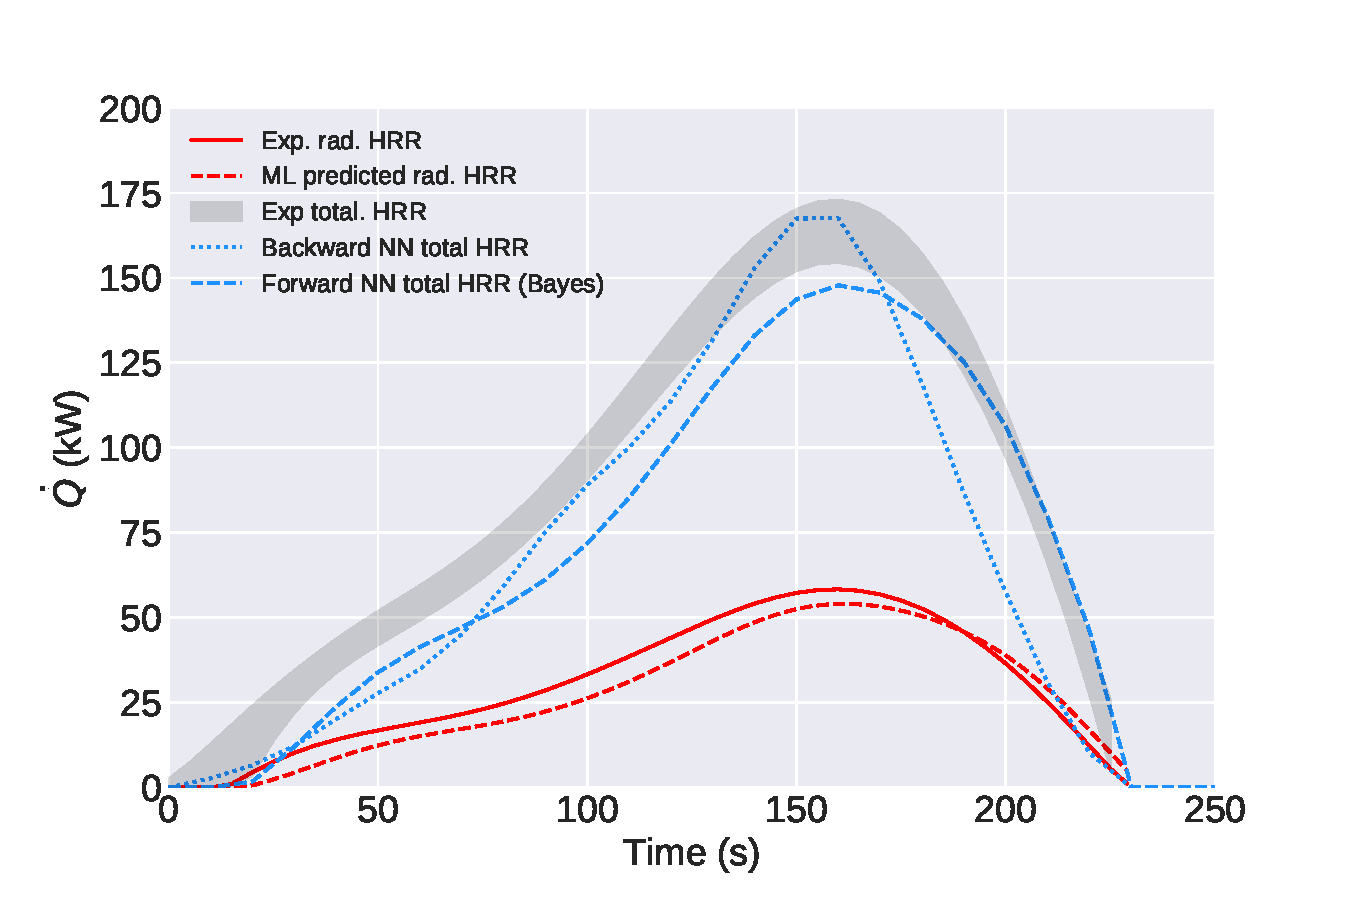
\includegraphics[width=\textwidth,keepaspectratio]{figures/nhex_12in_1_final.pdf}
      \caption{Forward: MAE = 14.4 kW (16.5 \%) \\ Backward: MAE = 16.0 kW (18.3 \%)}
      \label{fig:nhex_12in_1}
  \end{subfigure}
  \begin{subfigure}[t]{.45\textwidth}
      \centering
      \includegraphics[width=\textwidth ,keepaspectratio]{figures/nhex_12in_2_final.pdf}
      \caption{ Forward: MAE = 17.9 kW (28.7 \%) \\ Backward: MAE = 13.4 kW (21.4 \%)}
      \label{fig:nhex_12in_2}
  \end{subfigure}
  \caption{HRR inversion results for two n-Hexane pool fire experiments.} 
  \label{fig:nhex_fires}
\end{figure}

The results from the two methanol pool fires are shown in Figure \ref{fig:meth_fires}.

\begin{figure}[htbp]
  \centering
  \begin{subfigure}[t]{.45\textwidth}
      \centering
      \includegraphics[width=\textwidth,keepaspectratio]{figures/meth_22in_1_final.pdf}
      \caption{ Forward: MAE = 5.7 kW (10.0 \%) \\ Backward: MAE = 5.9 kW (10.5\%)}
      \label{fig:meth_22in_1}
  \end{subfigure}
  \begin{subfigure}[t]{.45\textwidth}
      \centering
      \includegraphics[width=\textwidth ,keepaspectratio]{figures/meth_22in_2_final.pdf}
      \caption{  Forward: MAE = 9.6 kW (15.9 \%) \\ Backward: MAE = 7.5 kW (12.5 \%)}
      \label{fig:meth_22in_2}
  \end{subfigure}
  \caption{HRR inversion results for two methanol pool fire experiments.} 
  \label{fig:meth_fires}
\end{figure}
\clearpage

The results show that the forward emulator approach generally outperforms the backward emulator approach. This is not surprising given that the forward emulator approach relies on heat flux measurements as opposed to only temperature measurements. The heat flux measurements constrain the shape of the HRR curve and the final result is scaled by $\frac{1}{\chi_R}$. When using the backward emulator approach, the output has no constraints and the HRR curve must be completely learned from the temperature measurements. A notable exception is the second n-Hexane pool fire experiment (Figure \ref{fig:nhex_12in_2}, in which the estimate of the radiative HRR does not agree well with the mass loss estimate, and as a result the forward emulator result exhibits similar errors.  

\section{Conclusions}
Heat release rate (HRR) inversion models are presented for fires with peak HRRs ranging from 80-200 kW using three different types of measurements- heat fluxes, video footage, and temperatures. The models are able to train on the data from three calibration experimental burner fires and are scored based on their ability to predict the transient HRR for an excluded ``test" experiment. A major advantage of the heat flux measurements is that they exhibit a linear relationship with the heat release rate if the measurements are taken from the same location and the fuel has a constant radiative fraction. This linear relationship allows for the use of a linear staticial model to predict the radiative component of the heat release rate. Because the input data has 33 features (DFTs), and they are correlated with each other, regularization is helpful to prevent overfitting. Also, it is not clear that all sensors are necessary, so a lasso regression is employed to both perform feature selection and make predictions. The lasso regression model includes mostly sensors that are close to the flame, both near the ground and near the ceiling. The predictions from the lasso model are temporally noisy, which motivates the use of a Gaussian process regression. This regression approach is a Bayesian method of computing a posterior distribution of underlying functions that are smoother than the raw lasso predictions. The use of the GPR reduces the mean absolute error (MAE) from 3.4 kW to 2.4 kW for the test experiment. The methodology is repeated using every experiment as the test case once, while using the remaining three experiments as the calibration set. The heat flux model produces estimates of the radiative HRR with MAEs ranging from 2.4 kW to 3.9 kW (9.3-11.2 \%). A similar approach is used based on video footage of the burner fires. For this model, the flame region is identified in a set of frames and the fraction of the field of view occupied by the frame is used as the predictor variable. It was found that the radiative HRR exhibits a fairly linear relationship with this quantity raised to the power of 4/3. A univariate linear regression is performed, which again produces temporally noisy estimates of the radiative HRR. A GPR is performed using the linear regression predictions as the input, and the final model produces estimates of the HRR with MAE values ranging from 1.4 kW to 6.8 kW (5.8-22.5\%). However, the MAE is 6.4 \% or less for three of the four tests; the test with the largest error exhibited a delayed ignition, which may hinder the accuracy of the model. The utility of the temperature measurements for HRR inversion is also explored. First, a computational analysis suggests that the thermocouple responses are relatively insensitive to the radiative fraction. This suggests that the thermocouple responses depend on the total HRR regardless of the radiative properties of the fuel used. Though this is a major advantage, developing a purely data-driven HRR inversion framework using the thermocouple responses is difficult because of hysteresis. Specifically, the measured temperature at an instant in time depends not only on the HRR at the same instant, but also on the history of the fire's growth. To model this hysteresis, Fire Dynamics Simulator (FDS), a CFD fire simulation model, is used. Because the runs can be computationally expensive and many runs can be required for the inversion framework, use of a coarse mesh is desirable. It was found that the simulated responses of thermocouples more than 1.5 m off the ground are relatively insensitive to the use of a coarse mesh, which results in a set of 17 thermocouples to be used for the inversion model. Even with the coarse mesh, each FDS simulation can take 20-30 minutes to run, which motivates the use of a faster way to produce the simulation results when new HRR predictions are desired. A set of artificial neural networks (ANN) are developed that learn the mapping from a transient HRR input and the set of transient thermocouple responses in FDS. A Gaussian process framework is used to construct the training set, which contains randomly generated HRR curves. Although this approach is computationally expensive because many runs are required to develop accurate ANN emulators, the use of transfer learning greatly reduces the number of required runs. The transfer learning used in this paper involves building a training set of 20,000 simulations from CFAST, a simplified two-zone fire model. Because of the simplified physics, a large training set of CFAST runs can be obtained much faster than an equivalent set of FDS runs. An ANN is first trained to produce the output of CFAST simulations, and the knowledge from this ANN is transferred to ANNs that learn to produce the output from FDS simulations. It was found that an ANN trained to emulate the simulated response of a thermocouple in FDS can produce more accurate results when it trains on 300 FDS runs with transfer learning than it can with 1,900 FDS runs and no transfer learning. Once the emulators are trained, they can produce the simulated responses of 17 thermocouples in FDS five orders of magnitude faster than it takes to achieve the results directly from FDS. The MAE of the emulator predictions is around 2 $^oC$, and they can produce predictions over 120 times per second. This gives the ability to quickly estimate the transient HRR for new experiments using various inversion methods. One method presented is a Bayesian parameter inversion on the fire's radiative fraction. Because the radiative HRR has already been estimated by the heat flux model, inverting for the radiative fraction allows for a simple calculation of the total HRR. This approach produces HRR estimates with MAEs that range 7.1 kW to 12.7 kW (8.7-12.7 \%) for burner fires and 5.7 kW to 17.9 kW (10.0-28.7 \%) for pool fires. The emulators can also be trained in the reverse direction in which they are trained to predict the HRR inputs to FDS that produces a simulated thermocouple response. This results in a set of estimated HRR curves based on a set of thermocouple responses. A ridge regression is performed to produce a weighted sum of the individual HRR estimates. This approach results HRR estimates with MAEs that range from 7.4 kW to 14.3 kW (8.7-14.7 \%) for burner fires and 5.9 kW to 16.0 kW (10.5-21.4 \%) for pool fires. 

\bibliographystyle{unsrtnat}
\bibliography{./references.bib}
\end{document}
